% !TeX encoding = UTF-8

%==============================================================================
% Arquivo principal do Trabalho de Conclusão de Curso
%==============================================================================

%==============================================================================
% DECLARAÇÃO DO TIPO DE DOCUMENTO
%==============================================================================
\documentclass{abnt-UDC-CC}

%==============================================================================
% PACOTES NECESSÁRIOS
%==============================================================================

% Utilizado em tabelas e quadros com células mescladas.
\usepackage{multirow}

% Permite controlar a posição de figuras com a opção [H].
\usepackage{float}

%==============================================================================
% PACOTES DESATIVADOS PARA REDUZIR O TEMPO DE COMPILAÇÃO
%
% Os diagramas do TCC são arquivos JPG/PNG inseridos por \includegraphics.
% Portanto, TikZ e PGFPlots não são necessários.
%==============================================================================
\usepackage{tikz}
\usetikzlibrary{positioning}
\usetikzlibrary{calc}
\usetikzlibrary{arrows.meta,shapes.geometric,fit,backgrounds}
\usetikzlibrary{decorations.pathreplacing}
% \usepackage{pgfplots}
% \pgfplotsset{compat=newest}

% Pacotes não utilizados no texto atual.
% \usepackage{adjustbox}
\usepackage{longtable}
% \usepackage{xtab}
% \usepackage[listofformat=subparens,subrefformat=parens,labelformat=parens]{subfig}
% \usepackage{lipsum}

%==============================================================================
% CAMINHOS PARA AS IMAGENS
%==============================================================================
\graphicspath{{./Imagens/}{./figuras/}{./Graficos/}}

%==============================================================================
% INFORMAÇÕES DO TRABALHO
%==============================================================================
% ---
% INFORMAÇÕES REFERENTE AO TCC
% ---

\titulo{Vulnerabilidades do IEEE 802.11 em ambientes IoT: estudo de caso utilizando microcontroladores de baixo custo}

\autor{Gustavo Mota do Nascimento}
\autorcitado{NASCIMENTO, Gustavo Mota}
\segundoautor{}
\segundoautorcitado{}
\terceiroautor{}
\terceiroautorcitado{}

\orientador{Luciano Santos Cardoso}
\orientadortitulo{Prof. Me.}
\coorientador{}
\coorientadortitulo{}

\profbancaum{\texorpdfstring{\PREENCHER}{[PREENCHER]}}
\profbancaumtitulo{}
\profbancadois{\texorpdfstring{\PREENCHER}{[PREENCHER]}}
\profbancadoistitulo{}
\instituicaoprofum{\texorpdfstring{\PREENCHER}{[PREENCHER]}}
\instituicaoprofdois{\texorpdfstring{\PREENCHER}{[PREENCHER]}}

\data{2026}
\databanca{\texorpdfstring{\PREENCHER}{[PREENCHER]}}

% codigoautor: atribuído pela biblioteca (ficha catalográfica)
\codigoautor{}
% codigopublicacao: atribuído pela biblioteca (ficha catalográfica)
\codigopublicacao{}

\palavrachaveum{IEEE 802.11}
\palavrachavedois{Desautenticação}
\palavrachavetres{Internet das Coisas}
\palavrachavequatro{Proteção de quadros de gerenciamento}

\textoresumo{%
	% TODO: escrever o resumo em português
}
\keywordum{}
\keyworddois{}
\keywordtres{}
\keywordquatro{}
\textoabstract{%
	% TODO: escrever o resumo em inglês
}
\textodedicatoria{%
	Dedico este trabalho à minha família, que sempre acreditou em mim.
}
\textoepigrafe{%
	``Segurança é um processo, não um produto.''

	Bruce Schneier
}
\textoagradecimento{%
	À minha família, pelo apoio e pela paciência durante toda a graduação.

	Ao meu orientador, Prof. Me. Luciano Santos Cardoso, pela orientação e pelas contribuições ao longo deste trabalho.

	Aos professores do curso de Ciência da Computação do Centro Universitário Dinâmica das Cataratas, pelos conhecimentos compartilhados.

	Aos amigos e colegas de curso, pela companhia e pelo incentivo nesta caminhada.
}

% ---
% INFORMAÇÕES DO CURSO E INSTITUIÇÃO
% ---

\local{Foz do Iguaçu}
\instituicao{Centro Universitário Dinâmica das Cataratas}
\instituicaoSigla{UDC}
% Natureza do documento final: usar o texto oficial exigido pela UDC.
\tipotrabalho{Trabalho de Conclusão de Curso}
\curso{Ciência da Computação}
\preambulo{\imprimirtipotrabalho\ apresentado como requisito obrigatório para obtenção do título de Bacharel em \imprimircurso\ do \imprimirinstituicao.}
\textoaprovacao{\imprimirtipotrabalho\ aprovado como requisito obrigatório para obtenção do título de Bacharel em \imprimircurso\ do \imprimirinstituicao, pela seguinte banca examinadora:}


%==============================================================================
% SEPARAÇÃO DE SÍLABAS
%==============================================================================
\hyphenation{Mar-ca-ção}
\hyphenation{mar-ca-ção}
\hyphenation{lin-gua-gem}
\hyphenation{pro-fis-sio-nais}
\hyphenation{ar-qui-vos}
\hyphenation{fer-ra-men-tas}
\hyphenation{ma-te-ri-al}

%==============================================================================
% MARCADORES DE REVISÃO (remover antes da versão final)
%==============================================================================
% Campo ainda não preenchido com dado real (não estimar).
\newcommand{\PREENCHER}{\textcolor{red}{\textbf{[PREENCHER]}}}
% Valor presente no texto, mas sob verificação nos logs pelo autor.
\newcommand{\CONFERIR}[1]{\textcolor{orange}{#1 \textbf{[CONFERIR]}}}
% Versão compacta dos marcadores, para uso dentro de tabelas estreitas:
% [PREENCHER] encolhe até caber na célula; [CONFERIR] vira o índice [C].
\newcommand{\marcadoTab}[1]{%
  \sbox0{\textcolor{red}{\textbf{#1}}}%
  \ifdim\wd0>\linewidth\resizebox{\linewidth}{!}{\usebox0}%
  \else\usebox0\fi}
\newcommand{\marcadoresTabela}{%
  \renewcommand{\PREENCHER}{\marcadoTab{[PREENCHER]}}%
  \renewcommand{\CONFERIR}[1]{\textcolor{orange}{##1\textsuperscript{\textbf{[C]}}}}}

% Coluna de largura fixa alinhada à esquerda (usada nas tabelas largas do Cap. 5).
\newcolumntype{L}[1]{>{\raggedright\arraybackslash}p{#1}}

%==============================================================================
% INÍCIO DO DOCUMENTO
%==============================================================================
\begin{document}

\frenchspacing

%==============================================================================
% ELEMENTOS PRÉ-TEXTUAIS
%==============================================================================

\imprimircapa

\imprimirfolhaderosto*

% Ficha catalográfica removida a pedido do autor (não exigida pela UDC).
% Para reativar, descomente a linha abaixo.
% \imprimirfichacatalografica

% Folha de aprovação removida a pedido do autor (banca/data ainda não definidas).
% Para reativar, descomente a linha abaixo e preencha a banca/data em Configuracoes/dados_documento.tex.
% \imprimirfolhadeaprovacao
\imprimirdedicatoria
\imprimiragradecimento
\imprimirepigrafe
% ---
% RESUMO PORTUGUÊS
% ---
\begin{resumo}[RESUMO]
\noindent A popularização de dispositivos da Internet das Coisas conectados por redes sem fio expõe esses equipamentos a vulnerabilidades legadas da família IEEE 802.11, entre elas a falsificação de quadros de gerenciamento quando a proteção definida na emenda 802.11w não é negociada. Este trabalho investiga como microcontroladores de baixo custo podem ser usados para testar essa vulnerabilidade em um ambiente com dispositivos conectados, com o objetivo de analisá-la e demonstrá-la em laboratório controlado. Trata-se de pesquisa aplicada, exploratória e descritiva, conduzida como estudo de caso experimental e restrita ao ataque de desautenticação. A bancada reuniu um roteador doméstico, uma plataforma de ataque baseada em microcontrolador, uma câmera, uma lâmpada, uma tomada e um \textit{smartphone} de referência, avaliados em duas configurações do ponto de acesso: sem proteção de quadros de gerenciamento e em modo misto, com proteção opcional. Os ensaios foram registrados por captura de quadros e por medidas de conectividade, e a segurança negociada por cada dispositivo foi verificada nos quadros de associação. Sem proteção, a câmera, a tomada, a lâmpada e o \textit{smartphone} apresentaram interrupções de conectividade expressivas, com recuperações distintas entre si. No modo misto, a câmera e a tomada negociaram o acesso sem proteção e voltaram a perder a conectividade, enquanto a lâmpada, que negociou proteção obrigatória, não apresentou interrupções. Conclui-se que o microcontrolador foi suficiente para testar a vulnerabilidade e que o padrão observado é compatível com a proteção esperada dos quadros de gerenciamento. O número reduzido de repetições e a ausência de uma condição WPA2 com proteção de quadros de gerenciamento impedem atribuir o efeito exclusivamente a esse mecanismo. Os resultados referem-se à disponibilidade dos dispositivos e não envolvem quebra de criptografia nem obtenção de credenciais.

 \vspace{\onelineskip}

 \noindent
 \textbf{Palavras-chave}: IEEE 802.11. Desautenticação. Internet das Coisas. Proteção de quadros de gerenciamento. ESP32-S3.
\end{resumo}

% ---
% RESUMO INGLÊS
% ---
\begin{resumo}[ABSTRACT]
 \begin{otherlanguage*}{english}
\noindent The spread of Internet of Things devices connected over wireless networks exposes them to legacy vulnerabilities of the IEEE 802.11 family, among them the forgery of management frames when the protection defined in amendment 802.11w is not negotiated. This work investigates how low-cost microcontrollers can be used to test this vulnerability in an environment with connected devices, aiming to analyze and demonstrate it in a controlled laboratory. It is applied, exploratory and descriptive research, conducted as an experimental case study and restricted to the deauthentication attack. The testbed comprised a home router, an attack platform based on a microcontroller, a camera, a smart bulb, a smart plug and a reference smartphone, evaluated under two access point configurations: without management frame protection and in mixed mode, with optional protection. The trials were recorded by frame capture and connectivity measurements, and the security negotiated by each device was verified in the association frames. Without protection, the camera, the plug, the bulb and the smartphone showed substantial connectivity interruptions, with distinct recoveries among them. In mixed mode, the camera and the plug negotiated access without protection and lost connectivity again, while the bulb, which negotiated mandatory protection, showed no interruptions. It is concluded that the microcontroller was sufficient to test the vulnerability and that the observed pattern is consistent with the expected protection of management frames. The small number of repetitions and the absence of a WPA2 condition with management frame protection prevent attributing the effect exclusively to this mechanism. The results concern device availability and involve neither breaking encryption nor obtaining credentials.

  \vspace{\onelineskip}

   \noindent
   \textbf{Keywords}: IEEE 802.11. Deauthentication. Internet of Things. Management frame protection. ESP32-S3.
 \end{otherlanguage*}
\end{resumo}


%==============================================================================
% LISTAS
%==============================================================================

\imprimirlistafiguras

\imprimirlistatabelas
\imprimirlistaquadros
% \imprimirlistagraficos
% \imprimirlistacodigos

\begin{siglas}
\item[ACK] \textit{Acknowledgement} (Confirmação de recebimento)
\item[AES] \textit{Advanced Encryption Standard} (Padrão Avançado de Criptografia)
\item[AKM] \textit{Authentication and Key Management} (Autenticação e Gerenciamento de Chaves)
\item[AP] \textit{Access Point} (Ponto de Acesso)
\item[BSSID] \textit{Basic Service Set Identifier} (Identificador do Conjunto Básico de Serviços)
\item[CCMP] \textit{Counter Mode with CBC-MAC Protocol}
\item[CNPq] Conselho Nacional de Desenvolvimento Científico e Tecnológico
\item[CRC] \textit{Cyclic Redundancy Check} (Verificação Cíclica de Redundância)
\item[CSMA/CA] \textit{Carrier Sense Multiple Access with Collision Avoidance}
\item[CSMA/CD] \textit{Carrier Sense Multiple Access with Collision Detection}
\item[DA] \textit{Destination Address} (Endereço de Destino)
\item[DCF] \textit{Distributed Coordination Function} (Função de Coordenação Distribuída)
\item[DIFS] \textit{Distributed Interframe Space}
\item[DSSS] \textit{Direct Sequence Spread Spectrum}
\item[EDCA] \textit{Enhanced Distributed Channel Access} (Acesso Distribuído Aprimorado ao Canal)
\item[ESP32-S3] SoC da Espressif com processador Xtensa LX7 e Wi-Fi em 2,4~GHz
\item[FC] \textit{Frame Control} (Controle de Quadro)
\item[FCS] \textit{Frame Check Sequence} (Sequência de Verificação de Quadro)
\item[FHSS] \textit{Frequency Hopping Spread Spectrum}
\item[GHz] Gigahertz
\item[GTK] \textit{Group Temporal Key} (Chave Temporal de Grupo)
\item[HCCA] \textit{HCF Controlled Channel Access} (Acesso ao Canal Controlado pela HCF)
\item[HCF] \textit{Hybrid Coordination Function} (Função de Coordenação Híbrida)
\item[HR/DSSS] \textit{High Rate Direct Sequence Spread Spectrum}
\item[ICMP] \textit{Internet Control Message Protocol}
\item[IDE] \textit{Integrated Development Environment} (Ambiente de Desenvolvimento Integrado)
\item[IEEE] \textit{Institute of Electrical and Electronics Engineers}
\item[IGTK] \textit{Integrity Group Temporal Key}
\item[IoT] \textit{Internet of Things} (Internet das Coisas)
\item[IP] \textit{Internet Protocol} (Protocolo de Internet)
\item[ISM] \textit{Industrial, Scientific and Medical}
\item[IV] \textit{Initialization Vector} (Vetor de Inicialização)
\item[LoRa] \textit{Long Range}
\item[MAC] \textit{Medium Access Control} (Controle de Acesso ao Meio)
\item[MFPC] \textit{Management Frame Protection Capable}
\item[MFPR] \textit{Management Frame Protection Required}
\item[MHz] Megahertz
\item[MIC] \textit{Message Integrity Code} (Código de Integridade de Mensagem)
\item[MIMO] \textit{Multiple-Input Multiple-Output}
\item[MMIE] \textit{Management MIC Information Element}
\item[NFC] \textit{Near-Field Communication} (Comunicação por Campo de Proximidade)
\item[OFDM] \textit{Orthogonal Frequency-Division Multiplexing}
\item[OSI] \textit{Open Systems Interconnection}
\item[OTA] \textit{Over-The-Air} (Atualização sem fio)
\item[PCF] \textit{Point Coordination Function} (Função de Coordenação Pontual)
\item[PHY] Camada física (\textit{Physical Layer})
\item[PMF] \textit{Protected Management Frames} (Quadros de Gerenciamento Protegidos)
\item[PMK] \textit{Pairwise Master Key}
\item[PNI] Programa Nacional de Imunizações
\item[PSK] \textit{Pre-Shared Key} (Chave Pré-Compartilhada)
\item[PTK] \textit{Pairwise Transient Key}
\item[RC4] \textit{Rivest Cipher 4}
\item[RFID] \textit{Radio-Frequency Identification} (Identificação por Radiofrequência)
\item[ROM] \textit{Read-Only Memory} (Memória Somente de Leitura)
\item[RSN] \textit{Robust Security Network}
\item[RSSI] \textit{Received Signal Strength Indicator} (Indicador de Intensidade do Sinal Recebido)
\item[RTS/CTS] \textit{Request to Send / Clear to Send}
\item[SA] \textit{Source Address} (Endereço de Origem); em \textit{SA Query}, \textit{Security Association}
\item[SAE] \textit{Simultaneous Authentication of Equals}
\item[SIFS] \textit{Short Interframe Space}
\item[SoC] \textit{System on a Chip} (Sistema em Chip)
\item[SRAM] \textit{Static Random-Access Memory}
\item[SSID] \textit{Service Set Identifier} (Identificador da Rede)
\item[STA] \textit{Station} (Estação / Dispositivo Cliente)
\item[TCP] \textit{Transmission Control Protocol}
\item[TKIP] \textit{Temporal Key Integrity Protocol}
\item[TWT] \textit{Target Wake Time}
\item[UDC] Centro Universitário Dinâmica das Cataratas
\item[USB] \textit{Universal Serial Bus}
\item[WEP] \textit{Wired Equivalent Privacy}
\item[WLAN] \textit{Wireless Local Area Network} (Rede Local Sem Fio)
\item[WPA] \textit{Wi-Fi Protected Access}
\item[WPA2] \textit{Wi-Fi Protected Access 2}
\item[WPA3] \textit{Wi-Fi Protected Access 3}
\end{siglas}


% \begin{simbolos}
  \item[$ \Gamma $] Letra grega Gama
  \item[$ \Lambda $] Lambda
  \item[$ \zeta $] Letra grega minúscula zeta
  \item[$ \in $] Pertence
\end{simbolos}


\imprimirsumario

%==============================================================================
% ELEMENTOS TEXTUAIS
%==============================================================================

\textual
\pagestyle{abnt_CC-UDC}

%==============================================================================
% CAPÍTULOS
%==============================================================================

% !TeX encoding = UTF-8
\chapter{Introdução}

O avanço da computação e a Quarta Revolução Industrial contribuíram para a popularização da Internet das Coisas (IoT) em ambientes residenciais e corporativos \cite{James2023}. O tema desta pesquisa insere-se no campo da segurança de redes e trata de vulnerabilidades do protocolo de comunicação sem fio IEEE 802.11 (Wi-Fi) quando aplicado a esses ambientes, utilizando um microcontrolador de baixo custo como plataforma de testes \cite{KristiyantoErnastuti2020}.

A literatura registra que a adoção da IoT trouxe ganhos de conveniência acompanhados de desafios de segurança em dispositivos residenciais, como câmeras IP e automações domésticas \cite{KristiyantoErnastuti2020}. Parte desses desafios decorre de restrições de \textit{hardware} adotadas para manter o baixo custo, como baixo poder de processamento, armazenamento limitado e restrições energéticas \cite{FarhadPyun2022}. Essas restrições, porém, não explicam sozinhas a exposição dos dispositivos: a política de atualização de \textit{firmware} de cada fabricante, as decisões de produto sobre quais mecanismos de segurança implementar e a configuração adotada pelo usuário na rede também determinam se um equipamento utiliza ou não proteções disponíveis no padrão \cite{Lima2025}.

Ao mesmo tempo, o próprio padrão IEEE 802.11 carrega vulnerabilidades legadas em sua camada MAC. A principal delas, para este trabalho, é a falta de proteção nativa --- criptografia e autenticação --- nas tramas de gerenciamento, conhecidas como \textit{management frames} \cite{KohliosHayajneh2018}. Quando a proteção de quadros de gerenciamento definida na emenda IEEE~802.11w (PMF) não é negociada, esses quadros circulam sem criptografia nem verificação de integridade, ficando expostos à falsificação.

Embora essas falhas estejam documentadas, ainda há poucos registros sobre como dispositivos IoT comerciais específicos reagem quando submetidos a ataques de desautenticação gerados por plataformas portáteis de baixo custo, e sobre como essa reação se relaciona com a segurança que cada dispositivo efetivamente negocia com o ponto de acesso.

\section{Problema de pesquisa}
\label{sec:problema}

Diante desse panorama, formula-se o seguinte problema de pesquisa: de que maneira microcontroladores de baixo custo podem ser explorados para identificar e testar vulnerabilidades no protocolo IEEE 802.11 em um ambiente composto por dispositivos IoT?

\section{Delimitação do estudo}
\label{sec:delimitacao}

O estudo restringe-se ao ataque de desautenticação, isto é, à transmissão de quadros de desautenticação forjados contra dispositivos associados a um ponto de acesso. O recorte experimental compreende:

\begin{itemize}
    \item uma única plataforma de ataque, a LILYGO T-Embed CC1101 Plus, baseada no ESP32-S3 e executando o \textit{firmware} Bruce;
    \item um único ponto de acesso (roteador TP-Link EX1500), na faixa de 2,4~GHz, canal 6;
    \item quatro dispositivos selecionados por conveniência: uma câmera IP, uma lâmpada inteligente, uma tomada inteligente e um \textit{smartphone} usado como referência;
    \item duas configurações de segurança do ponto de acesso: WPA2-PSK, isto é, \textit{Wi-Fi Protected Access 2} (WPA2) com \textit{Pre-Shared Key} (PSK), e o modo misto WPA2/WPA3, que acrescenta o \textit{Wi-Fi Protected Access 3} (WPA3);
    \item como evidências, capturas de tráfego IEEE~802.11 em modo monitor e registros de conectividade por \textit{ping}.
\end{itemize}

Ataques do tipo \textit{Evil Twin}, engenharia social e efeitos sobre o consumo de energia são discutidos no referencial teórico apenas como contexto e não foram testados. Da mesma forma, o monitoramento de câmaras de vacinas é tratado apenas como cenário de aplicação analítico, sem equipamentos de saúde na bancada. Os resultados valem para os equipamentos, versões e configurações efetivamente utilizados e não são generalizados para outros roteadores, dispositivos ou faixas de frequência.

\section{Justificativa}

A realização deste trabalho justifica-se pela necessidade de verificar, em um cenário aplicado, o efeito de técnicas de ataque acessíveis sobre dispositivos IoT de consumo. A difusão de ferramentas portáteis e baratas ampliou o acesso a técnicas capazes de interromper a conexão de dispositivos em redes locais; trabalhos recentes relatam o uso de ferramentas como o Flipper Zero e de plataformas baseadas em microcontroladores portáteis para explorar falhas em redes sem fio \cite{James2023,LitayemAlsadi2023}.

A expressão ``baixo custo'' é usada neste trabalho em sentido comparativo e de acessibilidade. A plataforma de ataque LILYGO T-Embed CC1101 Plus é uma placa de desenvolvimento baseada no microcontrolador ESP32-S3, comercializada no varejo de eletrônica e adquirível por qualquer pessoa, sem necessidade de equipamento especializado. O valor pago pelo autor na aquisição da plataforma foi de R\$~300,00 (trezentos reais), em 21 de setembro de 2026. Para comparação, o Flipper Zero, dispositivo portátil difundido em testes de segurança, custava US\$~169,00 na loja oficial do fabricante e, por não possuir rádio Wi-Fi, depende de uma placa de expansão (\textit{WiFi Devboard}) de US\$~35,00 para ataques ao IEEE~802.11, totalizando US\$~204,00 \cite{FlipperLoja}, o equivalente a aproximadamente R\$~1.200,00 pela cotação do dólar em novembro de 2026 \cite{BCBPtax2026}, sem frete e impostos de importação. A plataforma usada neste trabalho custou R\$~300,00, cerca de um quarto desse valor. Por ser portátil, autônoma e de aquisição simples, representa uma barreira de entrada muito menor do que a de montagens tradicionais de ataque, que dependem de um computador com adaptador em modo monitor e configuração específica. A instrumentação usada neste trabalho apenas para \emph{medir} o ataque --- o adaptador Wi-Fi AR9271, o \textit{notebook} com Kali Linux, o roteador e os dispositivos avaliados --- é distinta da plataforma de ataque e não é necessária para executá-lo.

Do ponto de vista prático, um ambiente com automação ou vigilância pode ter sua disponibilidade afetada por um atacante que utilize dispositivos acessíveis e de fácil transporte. Em ambientes críticos, como os de saúde, em que sensores conectados por Wi-Fi podem ser usados para monitorar a temperatura de vacinas, essa perda de disponibilidade poderia silenciar alarmes remotos; esse cenário é discutido de forma analítica, sem ensaio próprio, na Seção~\ref{subsec:cenario_vacinas}. Os resultados interessam a desenvolvedores de \textit{hardware}, administradores de rede e usuários, por indicarem a importância de adotar mecanismos de segurança disponíveis no padrão, como o PMF, e de considerar a disponibilidade dos dispositivos conectados ao escolher equipamentos e configurações.

Sob a perspectiva acadêmica, este trabalho apresenta-se como um estudo de caso comparativo e uma caracterização empírica: em ambiente laboratorial controlado, compara o comportamento de dispositivos IoT selecionados sob ataque de desautenticação, medindo o tempo sem resposta e a perda de associação, e relaciona esse comportamento à segurança efetivamente negociada por cada dispositivo na associação com o ponto de acesso. Esse registro da segurança negociada por dispositivo é o que este trabalho acrescenta ao estudo de \citeonline{KristiyantoErnastuti2020}, que também empregou câmera IP, ponto de acesso e microcontrolador em ataques de desautenticação.

\section{Objetivo geral}

Analisar e demonstrar, na prática, em um ambiente laboratorial controlado, as vulnerabilidades do protocolo IEEE 802.11 em dispositivos IoT comerciais, utilizando microcontroladores de baixo custo.

\section{Objetivos específicos}

\begin{enumerate}[label=\arabic*.]
    \item Configurar o ambiente de ataque, preparando microcontroladores de baixo custo da família ESP com \textit{firmwares} adequados para a injeção de pacotes.
    \item Executar testes de ataque de desautenticação contra os dispositivos alvo.
    \item Mensurar o tempo de indisponibilidade e o tempo de reconexão dos equipamentos sob diferentes cenários de ataque.
    \item Coletar e analisar os dados de tráfego capturados na rede para validar a eficácia técnica dos testes e documentar as falhas exploradas.
\end{enumerate}

\section{Organização do trabalho}

Além desta introdução, o trabalho está organizado em cinco capítulos e três apêndices. O Capítulo~\ref{cap:fund_teorico} apresenta o referencial teórico sobre o IEEE~802.11, os quadros de gerenciamento e o PMF, as plataformas da família ESP e as ameaças à IoT, além dos trabalhos relacionados. O Capítulo~\ref{cap:metodologia} descreve a classificação da pesquisa e os procedimentos de coleta e de análise. O Capítulo~\ref{cap:desenvolvimento} documenta o ambiente experimental: rede de teste, equipamentos, condições de execução, fluxograma e cadeia de processamento dos dados. O Capítulo~\ref{cap:analise_resultados} apresenta e discute os resultados, incluindo a segurança negociada por dispositivo e um cenário de aplicação analítico. O Capítulo~\ref{cap:conclusao} retoma o problema, o atendimento aos objetivos, as limitações e os trabalhos futuros. Por fim, os Apêndices~\ref{sec:evidencias-rsn}, \ref{sec:registro-execucoes} e~\ref{sec:protocolo} reúnem, respectivamente, as evidências da segurança negociada nas capturas, o registro dos ensaios por execução e o protocolo de execução dos ensaios.

% !TeX encoding = UTF-8
\chapter{Referencial teórico}
\label{cap:fund_teorico}

Este capítulo fundamenta os conceitos teóricos e técnicos necessários para a compreensão, execução e análise crítica da pesquisa proposta. A estrutura parte da apresentação das normas e dos mecanismos que regem a conectividade sem fio no padrão IEEE 802.11, com ênfase na camada de enlace e em seus mecanismos de acesso ao meio. Em seguida, analisa-se a arquitetura de ferramentas de \textit{hardware} ofensivo de baixo custo, em especial plataformas baseadas em microcontroladores. Por fim, discute-se o impacto técnico e sistêmico dessas vulnerabilidades no ecossistema da Internet das Coisas (IoT), com foco em ambientes residenciais. Todo o embasamento apresentado ancora-se no estado da arte da literatura acadêmica sobre segurança de redes, protocolos de comunicação e engenharia de microcontroladores \cite{KohliosHayajneh2018,Amoordon2022,Hiertz2010,Lima2025}.

\section{Segurança em redes sem fio e o protocolo IEEE 802.11}

\subsection{Evolução das normas e arquitetura da camada MAC}

O padrão IEEE 802.11, ratificado em 1997 pelo Instituto de Engenheiros Eletricistas e Eletrônicos (IEEE), estabeleceu as bases das redes locais sem fio (\textit{Wireless Local Area Networks} – WLAN) modernas. Sua evolução foi fortemente impulsionada pela necessidade de suportar volumes crescentes de tráfego de dados, mantendo a mobilidade dos nós e a flexibilidade de expansão das infraestruturas de telecomunicações \cite{Hiertz2010}. Nesse contexto, as primeiras emendas priorizaram o uso de faixas de radiofrequência não licenciadas, em especial as bandas ISM (\textit{Industrial, Scientific and Medical}) de 2{,}4~GHz e 5~GHz, e a melhoria progressiva da eficiência espectral e das taxas de transferência.

Do ponto de vista arquitetural, o IEEE 802.11 se apoia, principalmente, nas duas camadas inferiores do modelo de referência \textit{Open Systems Interconnection} (OSI): a camada física (PHY) e a camada de controle de acesso ao meio (MAC). Na camada física, \citeonline{Hiertz2010} descrevem a transição de esquemas de espectro espalhado relativamente simples e robustos a interferências, como o \textit{Direct Sequence Spread Spectrum} (DSSS) e o \textit{Frequency Hopping Spread Spectrum} (FHSS) do padrão original, de 1997, e o DSSS de alta taxa (HR/DSSS, \textit{High Rate DSSS}) da emenda 802.11b, para técnicas de modulação digital mais sofisticadas. O \textit{Orthogonal Frequency-Division Multiplexing} (OFDM), introduzido na emenda 802.11a, na faixa de 5~GHz, e levado aos 2,4~GHz pela emenda 802.11g, permitiu a divisão do sinal em múltiplas subportadoras ortogonais, aumentando significativamente a taxa efetiva de transmissão. Em seguida, a adoção de arranjos de múltiplas antenas (MIMO – \textit{Multiple-Input Multiple-Output}) a partir da emenda 802.11n viabilizou múltiplos fluxos espaciais em paralelo, elevando as taxas teóricas de aproximadamente 11~Mbit/s para patamares que podem ultrapassar a ordem de gigabits por segundo em versões mais recentes, como a 802.11ac \cite{Hiertz2010}.

Na camada MAC, por sua vez, a complexidade do protocolo reflete os desafios inerentes à transmissão pelo ar, um meio de difusão compartilhado, ruidoso e sujeito a colisões. Diferentemente das redes cabeadas baseadas em Ethernet (IEEE~802.3), que utilizam o mecanismo de detecção de colisões (CSMA/CD), o ambiente de radiofrequência impede que um nó perceba colisões de forma confiável enquanto transmite, devido à atenuação do sinal, ao efeito do nó oculto e ao fato de o transmissor mascarar sua própria recepção. Para contornar essa limitação, o IEEE 802.11 adota a \textit{Distributed Coordination Function} (DCF), responsável por implementar o mecanismo CSMA/CA (\textit{Carrier Sense Multiple Access with Collision Avoidance}) \cite{Hiertz2010}.

Nesse modelo, o dispositivo que deseja transmitir deve “escutar antes de falar” (\textit{listen-before-talk}), monitorando o meio antes de iniciar o envio de quadros. Se o canal permanecer livre por um intervalo denominado \textit{Distributed Interframe Space} (DIFS), a transmissão é iniciada; caso contrário, o dispositivo aguarda a liberação do meio e aplica um algoritmo de recuo exponencial (\textit{exponential backoff}) para reduzir a probabilidade de colisões subsequentes \cite{Hiertz2010}. Tal abordagem é fundamental para evitar a corrupção de quadros e garantir um nível mínimo de equidade no acesso ao meio. Entretanto, ela exige uma intensa troca de quadros de controle e de gestão para coordenar o acesso ao canal, de modo que a estabilidade da rede passa a depender diretamente da integridade e da autenticidade dessas mensagens de coordenação.

A Figura~\ref{fig:csma_ca} ilustra, de forma esquemática, o mecanismo CSMA/CA: a estação verifica o meio, aguarda o intervalo DIFS e, havendo disputa, aplica um recuo aleatório (\textit{backoff}) antes de transmitir o quadro, recebendo em seguida a confirmação (ACK) após um intervalo SIFS \cite{Hiertz2010}.

\begin{figure}[htb]
\centering
\caption{Mecanismo de acesso ao meio CSMA/CA com DIFS e \textit{backoff}}
\label{fig:csma_ca}
\resizebox{\textwidth}{!}{%
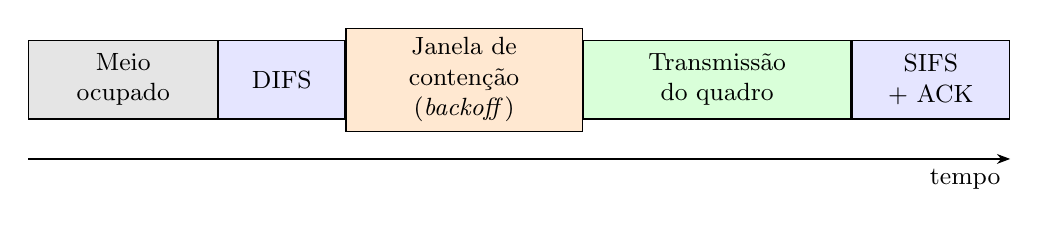
\begin{tikzpicture}[font=\small, seg/.style={draw, minimum height=10mm, align=center}]
\node[seg, fill=gray!20, minimum width=24mm] (busy) {Meio\\ocupado};
\node[seg, fill=blue!10, minimum width=16mm, right=0pt of busy] (difs) {DIFS};
\node[seg, fill=orange!18, minimum width=30mm, right=0pt of difs] (bo) {Janela de\\contenção\\(\textit{backoff})};
\node[seg, fill=green!15, minimum width=34mm, right=0pt of bo] (tx) {Transmissão\\do quadro};
\node[seg, fill=blue!10, minimum width=20mm, right=0pt of tx] (ack) {SIFS\\+ ACK};
\draw[-{Stealth}] ([yshift=-5mm]busy.south west) -- ([yshift=-5mm]ack.south east) node[below left]{tempo};
\end{tikzpicture}}
\legend{Fonte: elaborado pelo autor com base em Hiertz et al. (2010).}
\end{figure}

Ao longo das diversas emendas publicadas, a família 802.11 priorizou, de forma recorrente, ganhos de taxa de transmissão e de eficiência espectral em detrimento de uma preocupação inicial mais robusta com segurança. Emendas como 802.11b, 802.11g e 802.11n expandiram o uso de DSSS, OFDM e MIMO para atender à demanda crescente por aplicações multimídia, consolidando o Wi‑Fi como tecnologia predominante em ambientes residenciais e corporativos \cite{Hiertz2010}. Nesse processo, porém, a proteção das tramas de gerenciamento permaneceu limitada, o que resultou em uma base instalada de dispositivos com alta capacidade de transmissão, mas com superfícies de ataque relevantes ainda abertas na camada MAC, especialmente em relação à ausência de autenticação e integridade em quadros críticos de gestão \cite{KohliosHayajneh2018}.

A evolução temporal dos principais marcos da família IEEE~802.11 é sintetizada na Figura~\ref{fig:linha_tempo_80211}. A representação evidencia que o padrão foi ampliado para contemplar novas demandas de desempenho, interoperabilidade e segurança \cite{Hiertz2010}.

\begin{figure}[htb]
\centering
\caption{Principais marcos da evolução do padrão IEEE 802.11}
\label{fig:linha_tempo_80211}
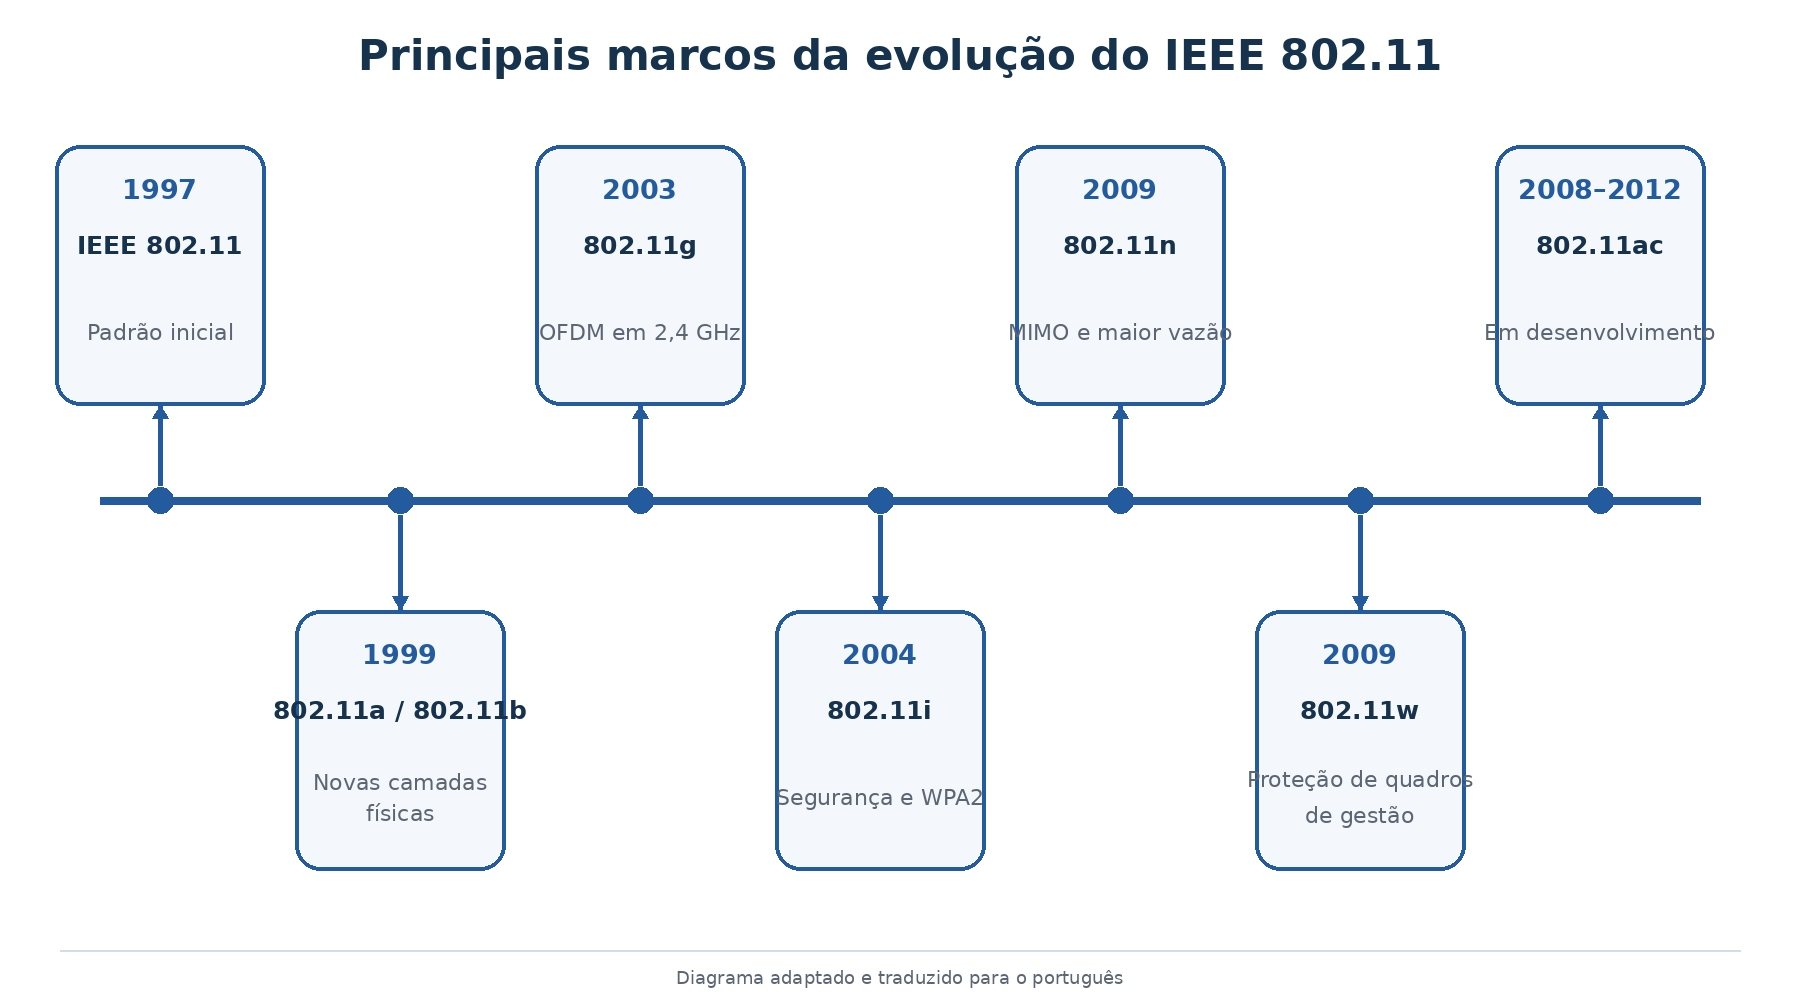
\includegraphics[width=0.96\textwidth]{linha_tempo_80211}
\legend{Fonte: adaptado de Hiertz et al. (2010).}
\end{figure}

Complementarmente à linha do tempo, a Figura~\ref{fig:emendas_mac_80211} organiza por área funcional as emendas do padrão, evidenciando os ramos de segurança (WEP, WPA, WPA2 e as emendas 802.11i e 802.11w), de qualidade de serviço (DCF; \textit{Point Coordination Function}, PCF; \textit{Hybrid Coordination Function}, HCF; e 802.11e) e de desempenho da camada física (802.11n, entre outras). Essa visão reforça que a proteção dos quadros de gerenciamento surge tardiamente na evolução do padrão, somente com a emenda 802.11w, o que é diretamente relevante para o objeto deste trabalho \cite{Hiertz2010,KohliosHayajneh2018}. Como \citeonline{Hiertz2010} é anterior ao WPA3, a inclusão desse ramo na figura apoia-se em \citeonline{KohliosHayajneh2018} e \citeonline{CiscoMFP2024}.

\begin{figure}[htb]
\centering
\caption{Emendas do padrão IEEE 802.11 organizadas por área funcional}
\label{fig:emendas_mac_80211}
\resizebox{\textwidth}{!}{%
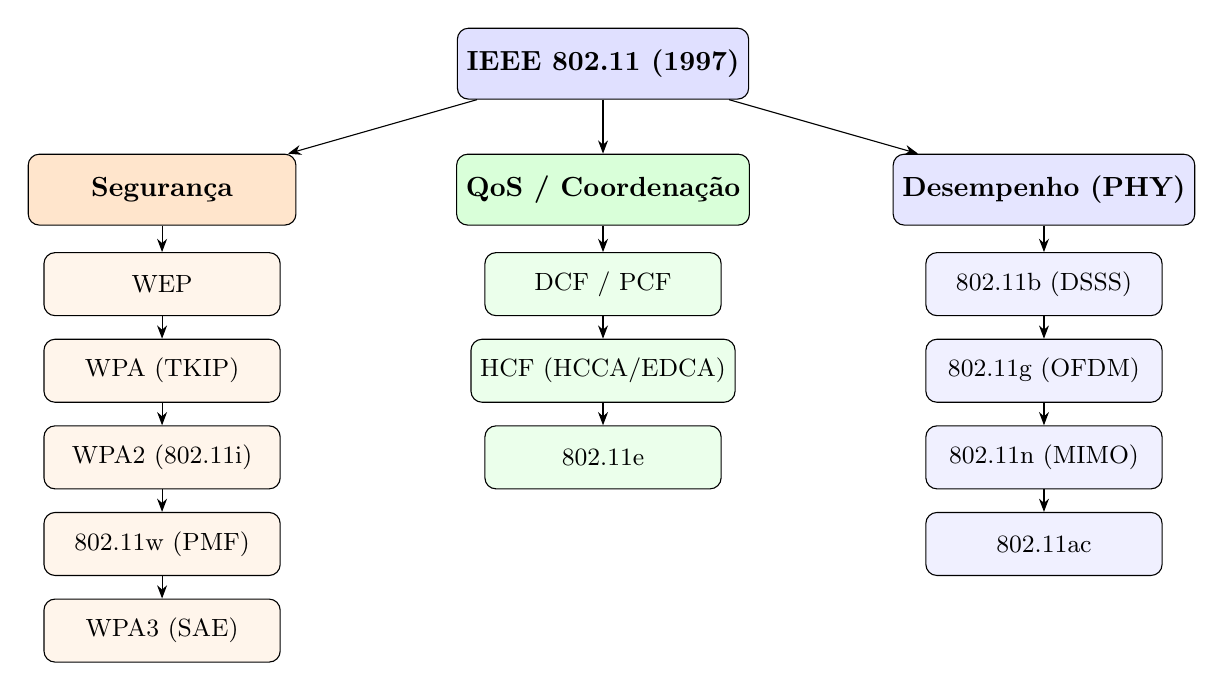
\begin{tikzpicture}[font=\small, >=Stealth,
  n/.style={draw, rounded corners, minimum width=30mm, minimum height=8mm, align=center},
  hdr/.style={draw, rounded corners, minimum width=34mm, minimum height=9mm, align=center, font=\bfseries}]
\node[hdr, fill=blue!12] (root) at (0,2.2) {IEEE 802.11 (1997)};
\node[hdr, fill=orange!20] (seg) at (-5.6,0.6) {Segurança};
\node[hdr, fill=green!15] (qos) at (0,0.6) {QoS / Coordenação};
\node[hdr, fill=blue!10] (phy) at (5.6,0.6) {Desempenho (PHY)};
\draw[->] (root) -- (seg);
\draw[->] (root) -- (qos);
\draw[->] (root) -- (phy);
\node[n, fill=orange!8] (wep) at (-5.6,-0.6) {WEP};
\node[n, fill=orange!8] (wpa) at (-5.6,-1.7) {WPA (TKIP)};
\node[n, fill=orange!8] (wpa2) at (-5.6,-2.8) {WPA2 (802.11i)};
\node[n, fill=orange!8] (w11) at (-5.6,-3.9) {802.11w (PMF)};
\node[n, fill=orange!8] (wpa3) at (-5.6,-5.0) {WPA3 (SAE)};
\draw[->] (seg) -- (wep); \draw[->] (wep) -- (wpa); \draw[->] (wpa) -- (wpa2); \draw[->] (wpa2) -- (w11); \draw[->] (w11) -- (wpa3);
\node[n, fill=green!8] (dcf) at (0,-0.6) {DCF / PCF};
\node[n, fill=green!8] (hcf) at (0,-1.7) {HCF (HCCA/EDCA)};
\node[n, fill=green!8] (e11) at (0,-2.8) {802.11e};
\draw[->] (qos) -- (dcf); \draw[->] (dcf) -- (hcf); \draw[->] (hcf) -- (e11);
\node[n, fill=blue!6] (b11) at (5.6,-0.6) {802.11b (DSSS)};
\node[n, fill=blue!6] (g11) at (5.6,-1.7) {802.11g (OFDM)};
\node[n, fill=blue!6] (n11) at (5.6,-2.8) {802.11n (MIMO)};
\node[n, fill=blue!6] (ac11) at (5.6,-3.9) {802.11ac};
\draw[->] (phy) -- (b11); \draw[->] (b11) -- (g11); \draw[->] (g11) -- (n11); \draw[->] (n11) -- (ac11);
\end{tikzpicture}}
\legend{Fonte: elaborado pelo autor com base em Hiertz et al. (2010), para as emendas até 802.11ac, e em \citeonline{KohliosHayajneh2018} e \citeonline{CiscoMFP2024}, para 802.11w e WPA3.}
\end{figure}

\subsection{Tramas de gestão e a ausência de criptografia nativa}

A comunicação na camada MAC do protocolo IEEE 802.11 não se restringe ao transporte do tráfego gerado pelas aplicações dos usuários. O tráfego é organizado em três classes principais de quadros (\textit{frames}): quadros de dados, quadros de controle e quadros de gestão (\textit{management frames}). Os quadros de dados carregam a carga útil (\textit{payload}) proveniente das camadas superiores; os quadros de controle incluem, por exemplo, confirmações de recebimento (ACK) e sinais de coordenação de acesso ao meio, como \textit{Request to Send/Clear to Send} (RTS/CTS); por fim, os quadros de gestão são responsáveis por funções como descoberta de redes, sincronização e estabelecimento ou encerramento de associações \cite{Amoordon2022}.

A organização dos quadros nessas três classes é sintetizada na Figura~\ref{fig:classes_quadros}, na qual se destacam os quadros de gestão, foco deste trabalho por concentrarem as tramas de desautenticação e dissociação \cite{Amoordon2022,KohliosHayajneh2018}.

\begin{figure}[htb]
\centering
\caption{Classes de quadros da camada MAC do IEEE 802.11}
\label{fig:classes_quadros}
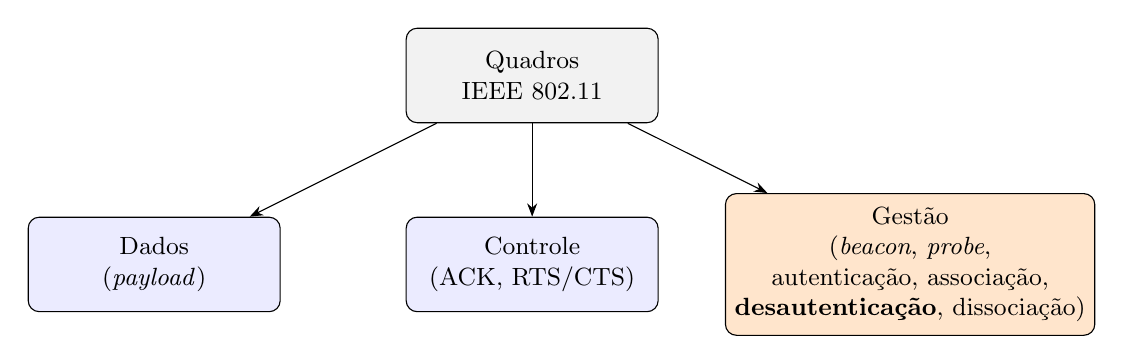
\begin{tikzpicture}[font=\small, every node/.style={align=center},
   box/.style={draw, rounded corners, minimum height=12mm, minimum width=32mm}]
\node[box, fill=gray!10] (root) at (0,0) {Quadros\\IEEE 802.11};
\node[box, fill=blue!8] (dados) at (-4.8,-2.4) {Dados\\(\textit{payload})};
\node[box, fill=blue!8] (ctrl) at (0,-2.4) {Controle\\(ACK, RTS/CTS)};
\node[box, fill=orange!20, minimum height=18mm] (gest) at (4.8,-2.4) {Gestão\\(\textit{beacon}, \textit{probe},\\autenticação, associação,\\\textbf{desautenticação}, dissociação)};
\draw[-{Stealth}] (root) -- (dados);
\draw[-{Stealth}] (root) -- (ctrl);
\draw[-{Stealth}] (root) -- (gest);
\end{tikzpicture}
\legend{Fonte: elaborado pelo autor com base em Amoordon et al. (2022) e Kohlios e Hayajneh (2018).}
\end{figure}

Segundo \citeonline{Amoordon2022}, os quadros de gestão constituem a espinha dorsal da conectividade sem fio, pois coordenam processos essenciais como autenticação e associação de estações (\textit{stations}, STA) a um ponto de acesso (AP – \textit{Access Point}). Entre os subtipos mais comuns, destacam‑se os \textit{beacons}, anúncios periódicos emitidos pelo AP que informam sua presença, o \textit{Service Set Identifier} (SSID) e as capacidades criptográficas suportadas; os \textit{probe requests} e \textit{probe responses}, utilizados por dispositivos clientes para sondar redes disponíveis; e as requisições de autenticação (\textit{authentication}) e associação (\textit{association}). Para a análise de segurança, assumem especial relevância as tramas de desautenticação (\textit{deauthentication}) e de dissociação (\textit{disassociation}), concebidas originalmente como mecanismos de encerramento ordenado de conexões, liberando memória, canais e \textit{buffers} associados a sessões específicas \cite{KohliosHayajneh2018}.

A estrutura de um quadro de gestão é rigidamente padronizada. O cabeçalho MAC (\textit{MAC Header}) contém, entre outros campos, o campo \textit{Frame Control} (FC), com 2~bytes, que indica a versão do protocolo, o tipo (\textit{Type}) e o subtipo (\textit{Subtype}) do quadro. Na sequência, são incluídos endereços de 6~bytes, correspondentes ao endereço de destino (\textit{Destination Address} – DA), ao endereço de origem (\textit{Source Address} – SA) e ao identificador do conjunto de serviços básico (BSSID), que, em redes de infraestrutura, representa o endereço MAC do próprio ponto de acesso. Após o cabeçalho, encontra‑se o corpo do quadro (\textit{Frame Body}), que pode incluir, por exemplo, o código de motivo (\textit{Reason Code}) associado a uma desautenticação. Por fim, o quadro é finalizado pela \textit{Frame Check Sequence} (FCS), campo que utiliza o algoritmo \textit{Cyclic Redundancy Check} de 32~bits (CRC‑32) para detecção de erros físicos ocorridos durante a transmissão pelo meio sem fio \cite{Lima2025}.

A Figura~\ref{fig:quadro_gestao} detalha esses campos para o caso em que o PMF (\textit{Protected Management Frames}, IEEE~802.11w) não é negociado. Nessa condição, o cabeçalho MAC e o corpo do quadro trafegam em texto claro, sem código de integridade de mensagem (MIC) ou outro mecanismo que comprove a autenticidade do emissor, e tornam-se passíveis de leitura e falsificação por qualquer dispositivo com capacidade de transmissão no canal \cite{KohliosHayajneh2018,Lima2025}. Quando o PMF é negociado, os quadros de gerenciamento classificados como robustos passam a ter proteção criptográfica, conforme discutido adiante.

\begin{figure}[htb]
\centering
\caption{Estrutura de um quadro de gerenciamento IEEE 802.11 sem PMF}
\label{fig:quadro_gestao}
\resizebox{\textwidth}{!}{%
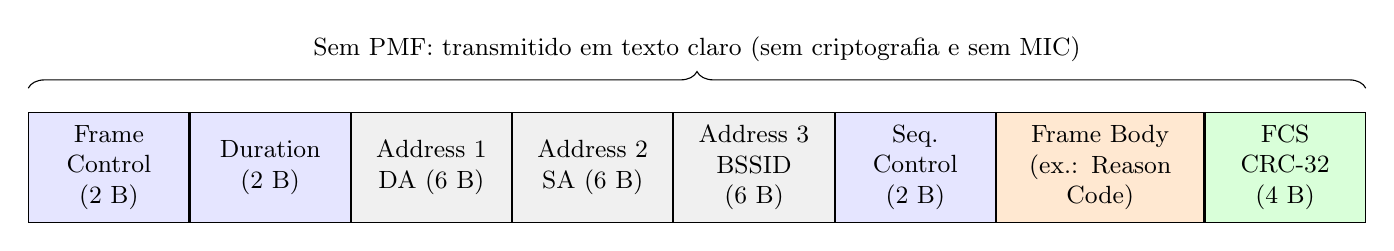
\begin{tikzpicture}[font=\small, f/.style={draw, minimum height=14mm, align=center, text width=18mm}]
\node[f, fill=blue!10] (fc) {Frame\\Control\\(2 B)};
\node[f, fill=blue!10, right=0pt of fc] (dur) {Duration\\(2 B)};
\node[f, fill=gray!12, right=0pt of dur] (a1) {Address 1\\DA (6 B)};
\node[f, fill=gray!12, right=0pt of a1] (a2) {Address 2\\SA (6 B)};
\node[f, fill=gray!12, right=0pt of a2] (a3) {Address 3\\BSSID (6 B)};
\node[f, fill=blue!10, right=0pt of a3] (sc) {Seq.\\Control\\(2 B)};
\node[f, fill=orange!18, right=0pt of sc, text width=24mm] (body) {Frame Body\\(ex.: Reason\\Code)};
\node[f, fill=green!15, right=0pt of body] (fcs) {FCS\\CRC-32\\(4 B)};
\draw[decorate, decoration={brace, amplitude=6pt}] ([yshift=3mm]fc.north west) -- ([yshift=3mm]fcs.north east) node[midway, above=6pt]{Sem PMF: transmitido em texto claro (sem criptografia e sem MIC)};
\end{tikzpicture}}
\legend{Fonte: elaborado pelo autor com base em Lima (2025), Kohlios e Hayajneh (2018) e \citeonline{CiscoMFP2024}. Representa um quadro sem PMF. Com PMF negociado, quadros robustos individuais (por exemplo, desautenticação) têm o corpo cifrado e autenticado, e os de difusão recebem um elemento MMIE com MIC; \textit{beacons}, \textit{probes}, autenticação e associação permanecem sem essa proteção.}
\end{figure}

A principal fragilidade histórica do IEEE 802.11 reside justamente na forma como esses campos são protegidos. Conforme apontam \citeonline{KohliosHayajneh2018}, os projetistas originais definiram que os quadros de gestão seriam transmitidos em texto claro (\textit{plaintext}), mesmo em redes configuradas com mecanismos de segurança. Essa decisão foi tomada para garantir que dispositivos clientes conseguissem identificar redes disponíveis, ler \textit{beacons} e negociar capacidades de conexão antes de receberem quaisquer chaves criptográficas. Como consequência, em redes WEP, WPA ou WPA2 que não negociam PMF, apenas a carga útil dos quadros de dados é efetivamente criptografada, enquanto o cabeçalho MAC e o corpo dos quadros de gestão permanecem expostos, sem código de integridade de mensagem (MIC) que comprove a autenticidade do emissor \cite{KohliosHayajneh2018,Lima2025}.

Essa condição, porém, não é uma propriedade fixa do WPA2. A emenda 802.11w do IEEE introduziu o PMF, que pode ser usado também com WPA2, de forma opcional ou obrigatória, e que se tornou obrigatório no WPA3. O PMF não protege todos os quadros de gestão, mas apenas os chamados quadros de gerenciamento robustos: desautenticação, dissociação e quadros \textit{Action} robustos (como os de \textit{SA Query}). Quadros individuais desse tipo passam a ser cifrados e autenticados com a chave da sessão; os de difusão recebem um código de integridade calculado com a \textit{Integrity Group Temporal Key} (IGTK), transportado no elemento MMIE (\textit{Management MIC Information Element}) \cite{CiscoMFP2024}. \textit{Beacons}, \textit{probes}, autenticação e associação, que ocorrem antes de existir chave de sessão, continuam sem essa proteção. A adoção do PMF é negociada em cada associação por meio de dois bits do elemento \textit{Robust Security Network} (RSN): \textit{Management Frame Protection Capable} (MFPC) e \textit{Management Frame Protection Required} (MFPR); o PMF só é usado quando a estação e o ponto de acesso declaram MFPC \cite{CiscoMFP2024}. Com PMF ativo, uma solicitação de associação de uma estação que já possui associação protegida é recusada temporariamente (\textit{status} 30) e verificada pelo procedimento de \textit{SA Query}, o que impede que um quadro forjado desfaça a sessão \cite{CiscoMFP2024}.

Na ausência do PMF, a falta de mecanismos de integridade e autenticação nesses quadros abriu um vetor importante para a injeção e a falsificação de tráfego. Manter quadros de gestão em texto claro contribuiu diretamente para o surgimento de ataques específicos ao protocolo, em especial aqueles que exploram tramas de desautenticação e dissociação forjadas \cite{KohliosHayajneh2018}. Em cenários em que qualquer emissor com capacidade de transmissão no canal pode construir pacotes com endereços MAC de origem e destino válidos, torna‑se viável induzir estações a encerrar sessões ativas sem necessidade de conhecer as credenciais da rede \cite{KohliosHayajneh2018,Lima2025}. Em ambientes densos e sem PMF, a repetição dessas tramas em alta frequência permite implementar ataques de negação de serviço capazes de derrubar múltiplos dispositivos simultaneamente com baixo esforço técnico \cite{Amoordon2022}, o que torna esse vetor particularmente atrativo para uso com microcontroladores de baixo custo.

O processo normal de conexão de uma estação envolve a passagem entre estados de autenticação e associação, como apresentado na Figura~\ref{fig:estados_autenticacao}. Quadros de desautenticação ou dissociação provocam o retorno da estação a estados anteriores, interrompendo a comunicação estabelecida \cite{KristiyantoErnastuti2020}.

\begin{figure}[htb]
\centering
\caption{Estados de autenticação e associação em uma rede IEEE 802.11}
\label{fig:estados_autenticacao}
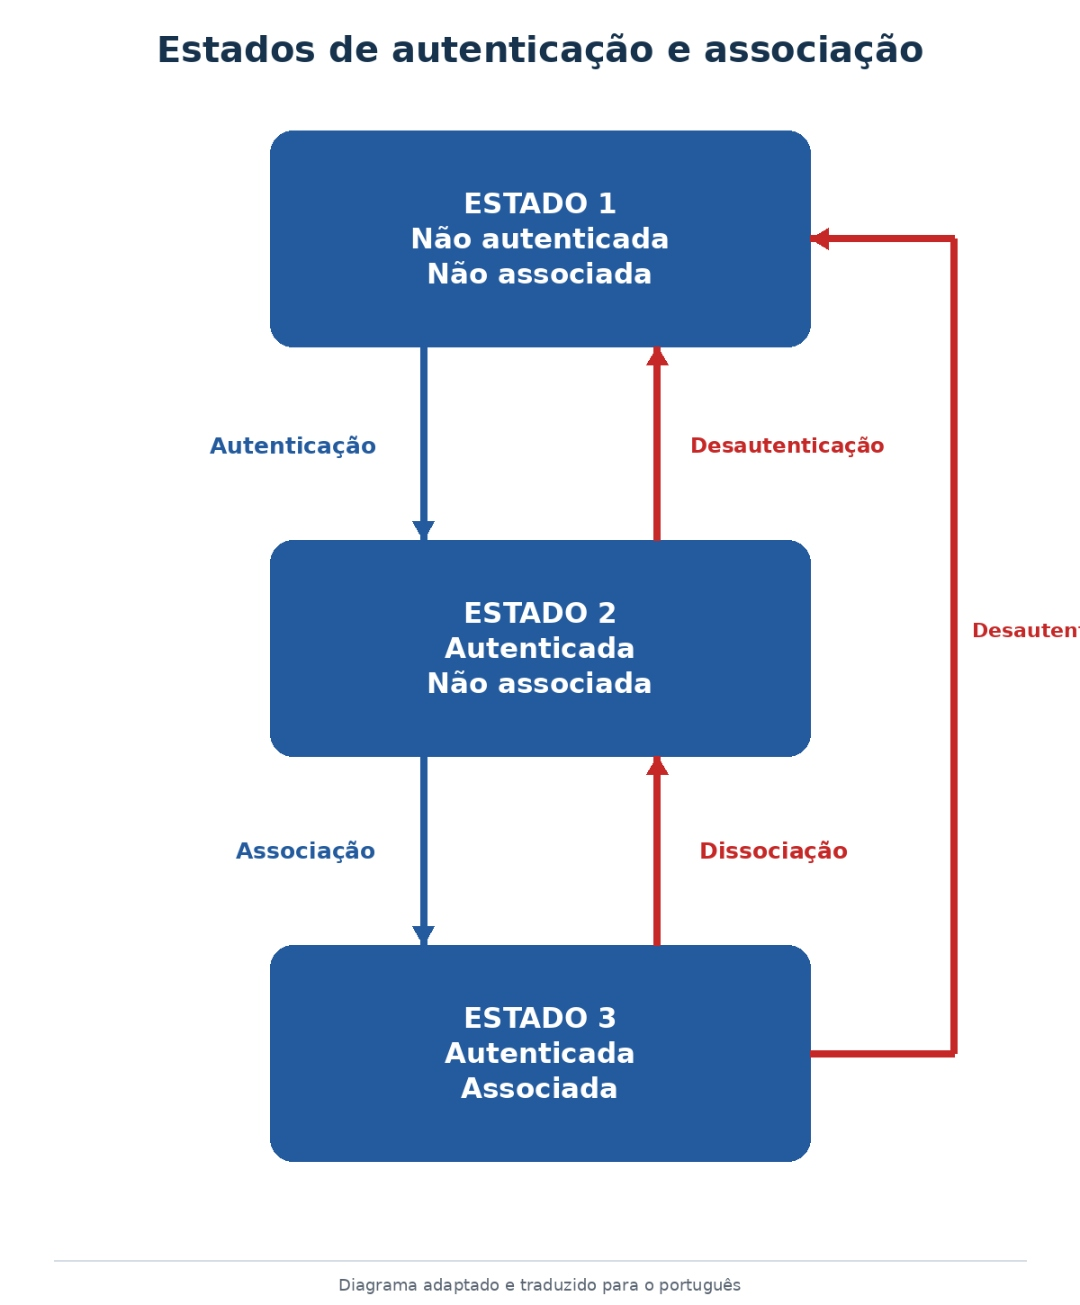
\includegraphics[width=0.53\textwidth]{estados_autenticacao}
\legend{Fonte: adaptado de Kristiyanto e Ernastuti (2020, p. 46).}
\end{figure}

\subsection{Evolução dos mecanismos de segurança: do WEP ao WPA3}

A segurança em redes IEEE 802.11 evoluiu ao longo do tempo em resposta direta à exploração das vulnerabilidades inerentes a um meio de transmissão aberto e suscetível à interceptação. O primeiro mecanismo padronizado foi o WEP (\textit{Wired Equivalent Privacy}), cujo objetivo era proporcionar um nível de confidencialidade considerado equivalente ao de redes cabeadas. O WEP baseava‑se na cifra de fluxo RC4 (\textit{Rivest Cipher 4}), associada a um código de redundância cíclica (CRC‑32) para verificação de integridade da carga útil \cite{KohliosHayajneh2018}.

A literatura, entretanto, evidencia falhas estruturais graves na concepção do WEP. O protocolo dependia de chaves estáticas, concatenadas a um vetor de inicialização (IV) de apenas 24~bits, transmitido em texto claro. Em redes com tráfego moderado ou elevado, o espaço reduzido de combinações para o IV era rapidamente esgotado, levando à sua inevitável reutilização. O reuso do IV, combinado com o fluxo de chaves gerado pelo RC4, possibilitou ataques estatísticos de criptoanálise e de recuperação passiva de chaves, permitindo que um invasor obtivesse a chave de rede em poucos minutos de tráfego capturado ou artificialmente injetado \cite{KohliosHayajneh2018,Lima2025}.

Essa experiência prática mostrou que a simples adoção de cifradores de fluxo não era suficiente para garantir confidencialidade, especialmente na ausência de um projeto cuidadoso de chaves e vetores de inicialização. A combinação de IVs curtos, chaves estáticas e reutilização de fluxos de chave tornou o WEP um mecanismo rapidamente obsoleto do ponto de vista de segurança \cite{KohliosHayajneh2018,Lima2025}. Para mitigar essas limitações sem substituir imediatamente o \textit{hardware} já instalado, a Wi‑Fi Alliance introduziu o WPA (\textit{Wi‑Fi Protected Access}) como solução transitória. O WPA passou a exigir o uso do \textit{Temporal Key Integrity Protocol} (TKIP), que modifica a forma de mistura de chaves e dos vetores de inicialização do RC4, gerando chaves dinâmicas por pacote. Além disso, incorporou um código de integridade de mensagem mais robusto, baseado no algoritmo Michael, com o objetivo de reduzir a injeção de quadros forjados e ataques de repetição \cite{KohliosHayajneh2018}.

Na sequência, o WPA2 consolidou o \textit{Advanced Encryption Standard} (AES) no modo \textit{Counter Mode with CBC-MAC Protocol} (CCMP), ou AES‑CCMP, como mecanismo padrão de proteção do tráfego de dados, elevando de forma significativa os níveis de confidencialidade e integridade em relação às versões anteriores. Apesar desses avanços, as tramas de gerenciamento permaneceram sem proteção equivalente nas redes WPA2 que não adotam PMF, de modo que, nelas, ataques de desautenticação e dissociação continuaram tecnicamente viáveis \cite{KohliosHayajneh2018}. A proteção sistemática de quadros de gestão veio com a emenda IEEE~802.11w (PMF), aplicável ao próprio WPA2, e foi reforçada pelo WPA3, que tornou o PMF obrigatório e adotou o protocolo SAE (\textit{Simultaneous Authentication of Equals}) \cite{CiscoMFP2024,EspressifWifiSecurity}.

No WPA2, o estabelecimento das chaves de sessão ocorre por meio do chamado \textit{4-way handshake}, executado após a autenticação inicial entre a estação (STA) e o ponto de acesso (AP). Nesse processo, ilustrado na Figura~\ref{fig:handshake_wpa2}, o AP envia um número aleatório (\textit{ANonce}); a STA responde com o seu próprio número (\textit{SNonce}) acompanhado de um código de integridade (MIC), o que permite a ambos derivarem a chave de sessão (\textit{Pairwise Transient Key} -- PTK); em seguida, o AP distribui a chave de grupo (\textit{Group Temporal Key} -- GTK) e a STA confirma a instalação das chaves. Somente após essa troca o tráfego de dados passa a ser cifrado com AES-CCMP \cite{KohliosHayajneh2018}. O \textit{4-way handshake}, por si só, protege os dados do usuário, mas não os quadros de gerenciamento. Quando o PMF é negociado, a terceira mensagem também entrega a IGTK, e as chaves derivadas nessa troca passam a proteger os quadros de gerenciamento robustos \cite{CiscoMFP2024}. O mesmo \textit{4-way handshake} é executado no WPA3-\textit{Personal}, como se discute a seguir.

\begin{figure}[htb]
\centering
\caption{Troca de chaves por \textit{4-way handshake} (WPA2 e WPA3-\textit{Personal})}
\label{fig:handshake_wpa2}
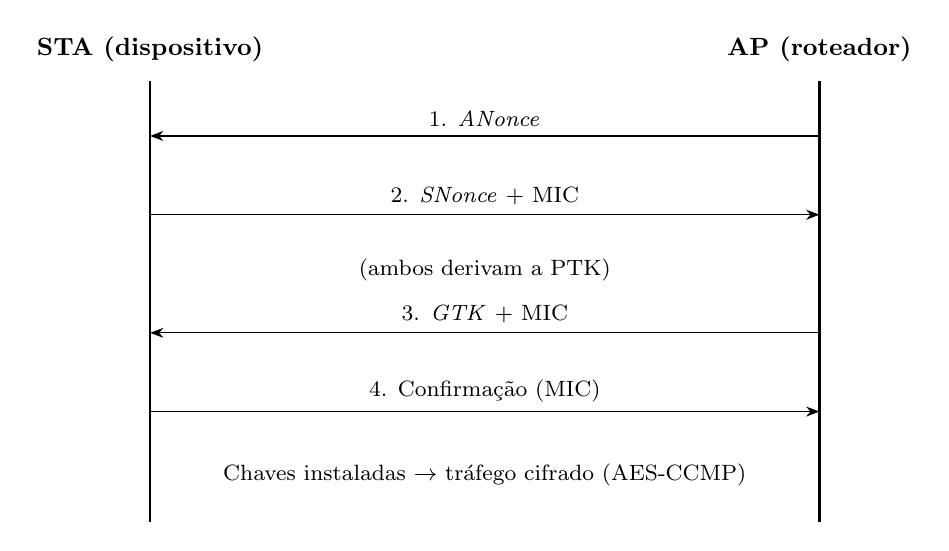
\begin{tikzpicture}[font=\small, >=Stealth]
\node (sta) at (0,0) {\textbf{STA (dispositivo)}};
\node (ap) at (8.5,0) {\textbf{AP (roteador)}};
\draw[thick] (0,-0.4) -- (0,-6);
\draw[thick] (8.5,-0.4) -- (8.5,-6);
\draw[->] (8.5,-1.1) -- node[above, font=\footnotesize]{1. \textit{ANonce}} (0,-1.1);
\draw[->] (0,-2.1) -- node[above, font=\footnotesize]{2. \textit{SNonce} + MIC} (8.5,-2.1);
\node[align=center, font=\footnotesize] at (4.25,-2.8) {(ambos derivam a PTK)};
\draw[->] (8.5,-3.6) -- node[above, font=\footnotesize]{3. \textit{GTK} + MIC} (0,-3.6);
\draw[->] (0,-4.6) -- node[above, font=\footnotesize]{4. Confirmação (MIC)} (8.5,-4.6);
\node[align=center, font=\footnotesize] at (4.25,-5.4) {Chaves instaladas $\rightarrow$ tráfego cifrado (AES-CCMP)};
\end{tikzpicture}
\legend{Fonte: elaborado pelo autor com base em Kohlios e Hayajneh (2018) e \citeonline{CiscoMFP2024}. A troca parte de uma PMK, derivada da senha no WPA2-PSK ou produzida pelo SAE no WPA3-\textit{Personal}. Com PMF negociado, a mensagem 3 também entrega a IGTK; sem PMF, os quadros de gerenciamento continuam desprotegidos após a troca.}
\end{figure}

O WPA3-\textit{Personal}, por sua vez, não elimina o \textit{4-way handshake}. O que o protocolo SAE (\textit{Simultaneous Authentication of Equals}), baseado em uma troca do tipo \textit{Dragonfly}, substitui é a autenticação baseada em PSK: em vez de a \textit{Pairwise Master Key} (PMK) ser derivada diretamente da senha, como no WPA2-PSK, ela é produzida por uma troca SAE realizada nos quadros de autenticação (\textit{authentication algorithm}~3), resistente a ataques de dicionário \textit{off-line}. Em seguida, o \textit{4-way handshake} é executado normalmente a partir dessa PMK para derivar as chaves de sessão \cite{KohliosHayajneh2018,EspressifWifiSecurity}. Além disso, o WPA3 torna obrigatório o PMF, que acrescenta integridade e autenticidade aos quadros de gerenciamento robustos, como os de desautenticação e dissociação, dificultando a sua falsificação. A Figura~\ref{fig:wpa3_sae_pmf} resume essas duas contribuições do WPA3 em relação às versões anteriores.

\begin{figure}[htb]
\centering
\caption{Principais contribuições de segurança do WPA3-\textit{Personal}}
\label{fig:wpa3_sae_pmf}
\resizebox{0.92\textwidth}{!}{%
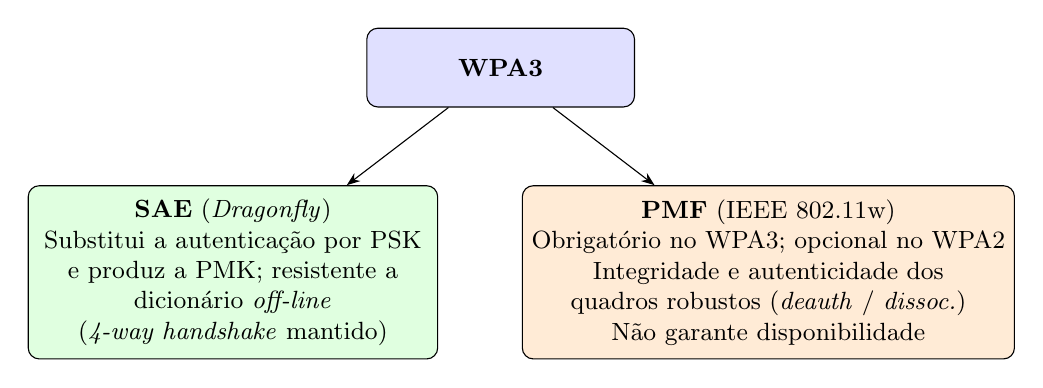
\begin{tikzpicture}[font=\small, >=Stealth,
  w/.style={draw, rounded corners, minimum width=52mm, minimum height=22mm, align=center}]
\node[w, fill=blue!12, minimum width=34mm, minimum height=10mm] (root) at (0,2) {\textbf{WPA3}};
\node[w, fill=green!12] (sae) at (-3.4,-0.6) {\textbf{SAE} (\textit{Dragonfly})\\Substitui a autenticação por PSK\\e produz a PMK; resistente a\\dicionário \textit{off-line}\\(\textit{4-way handshake} mantido)};
\node[w, fill=orange!16] (pmf) at (3.4,-0.6) {\textbf{PMF} (IEEE 802.11w)\\Obrigatório no WPA3; opcional no WPA2\\Integridade e autenticidade dos\\quadros robustos (\textit{deauth} / \textit{dissoc.})\\Não garante disponibilidade};
\draw[->] (root) -- (sae);
\draw[->] (root) -- (pmf);
\end{tikzpicture}}
\legend{Fonte: elaborado pelo autor com base em Kohlios e Hayajneh (2018), \citeonline{CiscoMFP2024} e \citeonline{EspressifWifiSecurity}. O PMF impede a falsificação de quadros robustos, mas não protege contra interferência física (\textit{jamming}) nem contra outras formas de negação de serviço por rádio.}
\end{figure}

Na prática, contudo, a adoção desses mecanismos é desigual, sobretudo em ambientes compostos por dispositivos IoT de baixo custo. Muitos equipamentos legados não dispõem de recursos de \textit{hardware} ou de espaço de \textit{firmware} suficientes para suportar plenamente PMF e WPA3 \cite{Lima2025}. A permanência de dispositivos legados sem suporte a WPA3 leva, na prática, ao uso de modos de compatibilidade, como o modo de transição WPA2/WPA3. É importante notar, contudo, que a segurança não é definida para a rede como um todo: no modo de transição, o ponto de acesso anuncia mais de um conjunto de autenticação (PSK e SAE) e o PMF como opcional, como registrado nas capturas deste trabalho (Apêndice~\ref{sec:evidencias-rsn}); com o PMF opcional, estações que não suportam o IEEE~802.11w continuam autorizadas a se conectar \cite{CiscoMFP2024}, e cada estação negocia, na sua própria associação, o \textit{Authentication and Key Management} (AKM) e o uso do PMF que suporta. Assim, um dispositivo legado que negocia WPA2-PSK sem PMF permanece exposto à falsificação de quadros de gestão, sem que isso retire a proteção das estações que negociaram SAE e PMF na mesma rede. O risco do modo de transição está, portanto, na permanência de associações desprotegidas, e não em um rebaixamento automático de todas as estações, o que é especialmente relevante em redes residenciais com muitos dispositivos IoT de baixo custo \cite{Hassija2019,Lima2025}. Os resultados deste trabalho ilustram essa negociação por associação (Seção~\ref{subsec:consolidacao_resultados}).

Em síntese, a evolução do IEEE 802.11 demonstra um avanço consistente nos mecanismos de proteção do tráfego de dados, mas revela também uma defasagem histórica na proteção das tramas de gerenciamento. Essa assimetria cria uma superfície de ataque particularmente sensível: nas associações que não negociam PMF, quadros de desautenticação e dissociação podem ser forjados e injetados no meio por qualquer dispositivo com capacidade de transmissão em nível MAC. No contexto deste trabalho, essa característica é explorada experimentalmente por meio de microcontroladores de baixo custo, que atuam como vetores de ataque contra dispositivos IoT em cenários residenciais.

A evolução dos mecanismos de segurança é apresentada na Figura~\ref{fig:evolucao_seguranca_80211}. O diagrama relaciona WEP, WPA, WPA2, IEEE~802.11w e WPA3, destacando o fortalecimento progressivo da proteção dos dados e, posteriormente, dos quadros de gerenciamento \cite{Hiertz2010,KohliosHayajneh2018,CiscoMFP2024}. A sequência não deve ser lida como uma separação rígida entre WPA2 desprotegido e WPA3 protegido: o PMF do IEEE~802.11w pode ser usado com WPA2, é obrigatório no WPA3 e, em ambos os casos, é negociado em cada associação \cite{CiscoMFP2024}.

\begin{figure}[htb]
\centering
\caption{Evolução dos mecanismos de segurança no padrão IEEE 802.11}
\label{fig:evolucao_seguranca_80211}
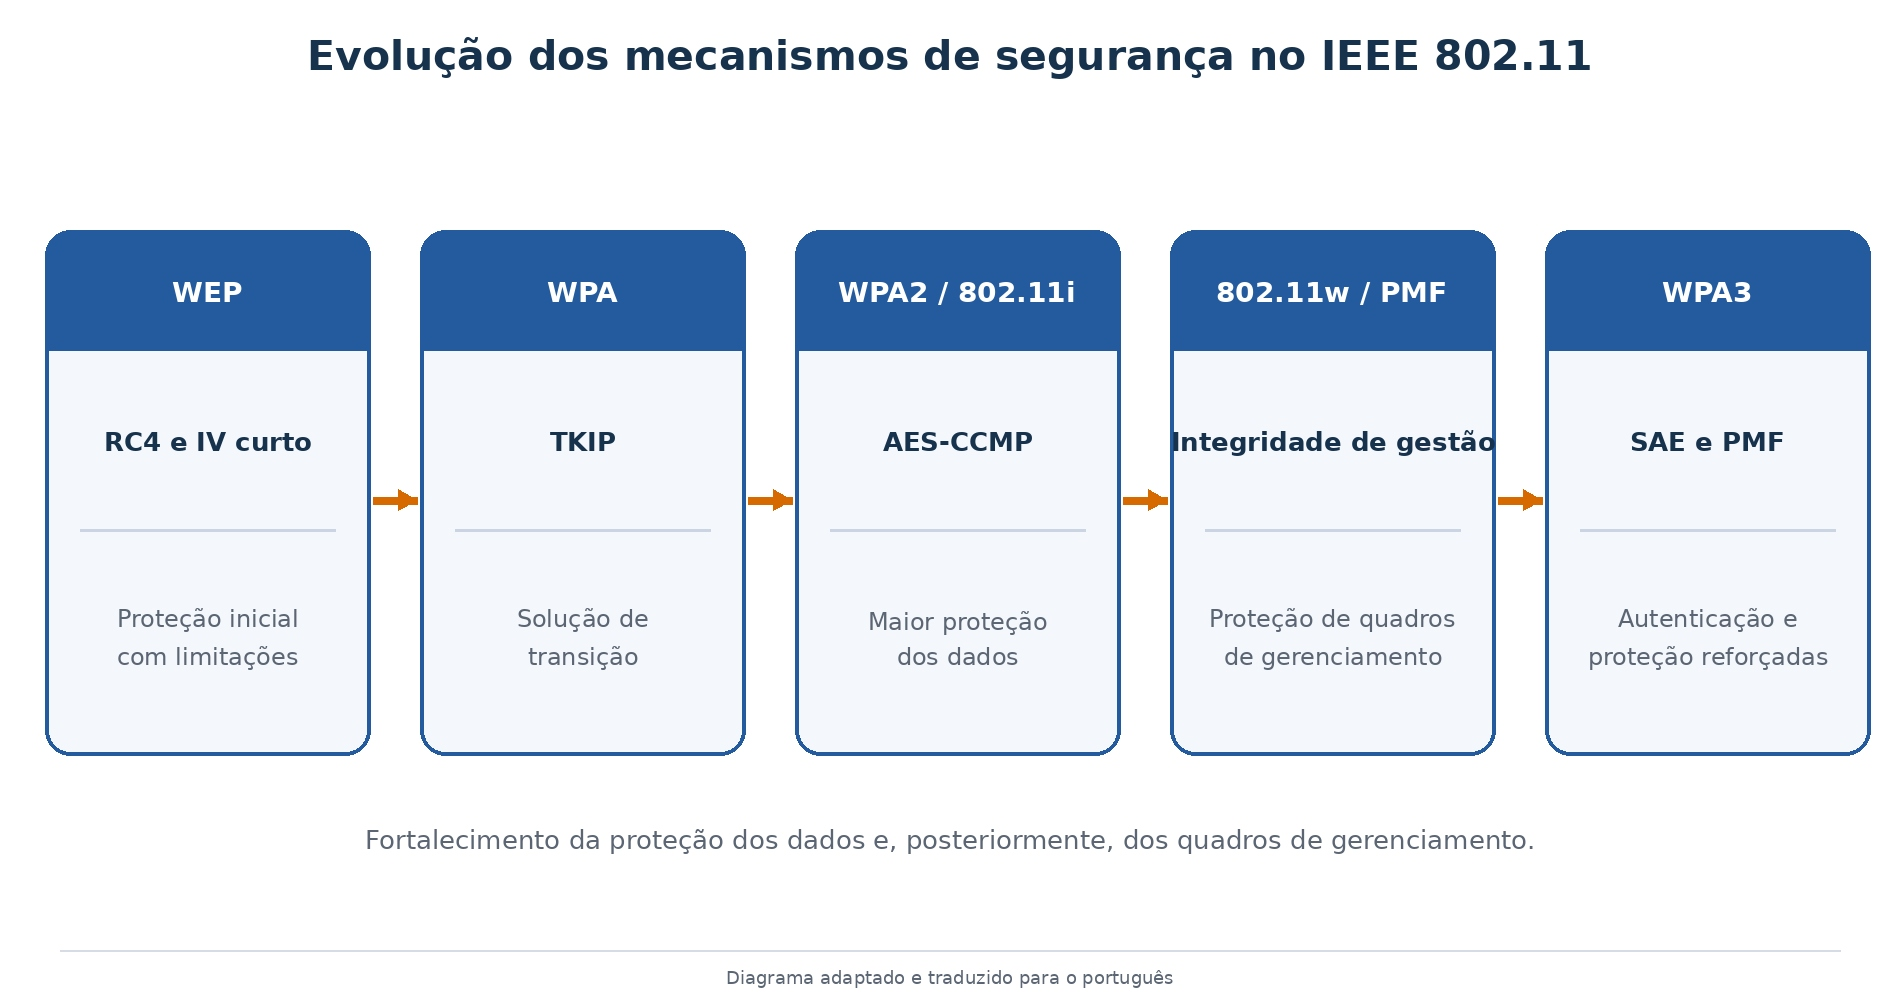
\includegraphics[width=0.98\textwidth]{evolucao_seguranca_80211}
\legend{Fonte: elaborado pelo autor com base em Hiertz et al. (2010), para WEP, WPA e WPA2, e em \citeonline{KohliosHayajneh2018} e \citeonline{CiscoMFP2024}, para 802.11w e WPA3. O IEEE~802.11w (PMF) é opcional no WPA2 e obrigatório no WPA3; protege apenas quadros de gerenciamento robustos e só vale para as associações que o negociam.}
\end{figure}

\section{Microcontroladores e hardware ofensivo de baixo custo}

\subsection{Arquitetura de hardware das plataformas ESP8266, ESP32 e ESP32-S3}

O barateamento e a miniaturização de componentes semicondutores deram origem a sistemas em chip (SoC) com alta capacidade de processamento e conectividade, que atualmente constituem parte essencial da indústria de IoT. Nesse contexto, as plataformas fabricadas pela Espressif Systems, notadamente o ESP8266, o ESP32 e o ESP32-S3, destacam-se pela relação custo-benefício e pela ampla adoção em projetos comerciais e acadêmicos.

\citeonline{LitayemAlsadi2023} exploram em detalhe a arquitetura dessas plataformas. O ESP8266 é baseado no microprocessador L106, de 32~bits da Tensilica, operando tipicamente a 80~MHz, com cerca de 160~kB de \textit{Static Random-Access Memory} (SRAM) e integração nativa do protocolo IEEE~802.11 b/g/n, suportando integralmente a pilha \textit{Transmission Control Protocol}/\textit{Internet Protocol} (TCP/IP). Essa integração elimina a necessidade de \textit{chipsets} adicionais para conectividade Wi-Fi, reduzindo custos e complexidade de projeto. O ESP32 representa um salto arquitetural significativo: incorpora processador Xtensa Dual-Core LX6 de 32~bits, SRAM expandida para aproximadamente 520~kB, além de módulos combinados de Wi‑Fi e Bluetooth, tanto em modo clássico quanto em \textit{Low Energy} \cite{LitayemAlsadi2023}.

O ESP32-S3, utilizado neste trabalho por meio da placa LILYGO T-Embed CC1101 Plus, não deve ser confundido com o ESP32 original. Trata-se de um SoC posterior, com processador Xtensa LX7 de 32~bits e dois núcleos, de até 240~MHz, 512~kB de SRAM, Wi-Fi IEEE~802.11 b/g/n restrito à faixa de 2,4~GHz (canais de 20 e 40~MHz) e Bluetooth \textit{Low Energy} 5, sem o Bluetooth clássico do ESP32 \cite{EspressifS3Datasheet}. Em todos esses casos, trata-se de SoCs com rádio 802.11 embutido, capazes de executar aplicações e controlar diretamente a interface sem fio.

A facilidade de programação desses microcontroladores, suportada por ambientes como Arduino IDE, PlatformIO e MicroPython, somada à capacidade de realizar atualizações \textit{Over-The-Air} (OTA), tornou essas plataformas particularmente adequadas para o desenvolvimento rápido de aplicações conectadas. Do ponto de vista da engenharia de segurança, o mesmo conjunto de características — baixo custo, alta disponibilidade e acesso direto ao transceptor Wi‑Fi — favorece seu emprego em experimentos de segurança ofensiva, notadamente em cenários de testes de intrusão em redes IEEE~802.11 e em estudos sobre a exploração de vulnerabilidades em tramas de gerenciamento.

\subsection{Modos de operação: modo estação, \textit{access point} e modo monitor}

As plataformas ESP possuem uma pilha de rádio flexível, capaz de operar em múltiplos estados lógicos, o que permite contornar parte das camadas tradicionais de rede \cite{LitayemAlsadi2023}. Os modos operacionais padrão incluem o modo estação (STA), no qual o microcontrolador atua como cliente conectando-se a um roteador Wi‑Fi existente, e o modo \textit{Access Point} (AP), em que o próprio chip passa a atuar como ponto de acesso, fornecendo endereços IP e hospedando uma rede local. Esse último modo é também explorado em cenários de \textit{Evil Twin}, nos quais um AP falso imita o identificador de serviço (SSID) e outros parâmetros do roteador legítimo, com as restrições discutidas na Seção~\ref{subsec:evil_twin}.

Para fins de auditoria de segurança, destaca-se a captura de quadros do canal, que exige distinguir dois conceitos frequentemente confundidos. No modo promíscuo, a interface, associada a uma rede, deixa de descartar os quadros daquela rede que não são destinados ao seu endereço MAC e os repassa ao sistema. No modo monitor, a interface não precisa estar associada: ela entrega todos os quadros IEEE~802.11 recebidos no canal sintonizado, inclusive quadros de gerenciamento e de controle e quadros de outras redes, com o cabeçalho 802.11 original. Para a análise de quadros de desautenticação e de associação, o modo relevante é o monitor, empregado neste trabalho com o adaptador AR9271. Nos chips da Espressif, essa função é oferecida pelo próprio \textit{framework} oficial como modo \textit{sniffer}, que, apesar de ser ativado por uma função chamada \texttt{esp\_wifi\_set\_promiscuous}, entrega quadros de gerenciamento, de dados e de controle e pode operar sem associação \cite{EspressifWifiModes}. Essa funcionalidade concede ao dispositivo a capacidade de atuar como um \textit{sniffer} de pacotes, extraindo cabeçalhos de comunicação da vizinhança sem fio \cite{Lima2025}. Na prática, isso permite identificar BSSIDs, endereços MAC de estações, tipos de quadros de gerenciamento e parâmetros de configuração de redes alvo, insumos essenciais para a construção de ataques de desautenticação direcionados.

\subsection{Injeção de pacotes e \textit{bypassing} de protocolos via hardware programável}

A capacidade de injeção de pacotes (\textit{packet injection}) representa o complemento ofensivo do modo monitor. Enquanto o modo monitor permite apenas a escuta passiva do meio, a injeção torna possível construir arbitrariamente sequências de bytes na memória do microcontrolador e transmiti-las diretamente pelo ar, ignorando parte do controle de estado normalmente imposto pela pilha de rede do sistema operacional. Em outras palavras, o microcontrolador deixa de seguir o fluxo convencional de associação, autenticação e estabelecimento de sessão, passando a emitir quadros IEEE~802.11 “sob medida” em nível MAC.

Ferramentas de código aberto, como o projeto \textit{esp8266\_deauther}, empacotam essas instruções de baixo nível em bibliotecas de uso relativamente simples. \citeonline{LitayemAlsadi2023} destacam que essas aplicações, muitas vezes disponibilizadas em repositórios públicos, transformam um chip de custo extremamente reduzido em um vetor de ataque efetivo. Ao manipular diretamente a interface de programação de aplicações do módulo Wi‑Fi da Espressif, o \textit{software} contorna validações usuais, construindo tramas de desautenticação a partir de endereços MAC obtidos previamente em captura de tráfego e efetivando, contra estações que não negociaram PMF, ataques de negação de serviço sem necessidade de \textit{hardware} profissional dedicado. Assim, funções originalmente concebidas para testes de laboratório ou desenvolvimento acabam sendo reutilizadas em contextos ofensivos, democratizando o acesso a técnicas antes restritas a equipamentos especializados.

\subsection{Ferramentas portáteis e a democratização do \textit{pentesting}}

O \textit{pentesting} sem fio, antes associado a \textit{notebooks} com distribuições Linux e adaptadores específicos, passou a contar com dispositivos portáteis de baixo custo. O Flipper Zero é um exemplo conhecido: reúne funções em Sub-1~GHz, \textit{Radio-Frequency Identification} (RFID), \textit{Near-Field Communication} (NFC) e infravermelho e, para Wi-Fi, depende de módulos externos baseados em ESP8266 ou ESP32, que realizam varreduras e ataques de desautenticação sem computador auxiliar \cite{James2023}. Esse trabalho é um \textit{preprint} que, segundo o próprio documento, não passou por revisão por pares; por isso, é usado aqui apenas para descrever a categoria da plataforma, e não como evidência de desempenho. A plataforma usada neste trabalho, a LILYGO T-Embed CC1101 Plus com \textit{firmware} Bruce, segue a mesma lógica, mas integra o ESP32-S3 na própria placa. Essa portabilidade indica que dispositivos da família ESP são, ao mesmo tempo, representativos do desenvolvimento IoT e instrumentos viáveis para ensaios de desautenticação em laboratório \cite{LitayemAlsadi2023}.

\section{Internet das Coisas e vulnerabilidades de borda}

\subsection{Definições e arquiteturas de redes de sensores}

O termo Internet das Coisas refere-se à rede global de dispositivos físicos incorporados a eletrônica, \textit{software} e sensores, que lhes conferem a capacidade de adquirir, processar e transferir dados sobre o ambiente e sobre sua própria operação. \citeonline{LiXuZhao2015} descrevem a arquitetura clássica da IoT como um modelo estratificado em três camadas principais: camada de percepção, camada de rede e camada de aplicação.

A camada de percepção é composta por nós terminais, como câmeras, sensores de temperatura, atuadores e etiquetas RFID, responsáveis por interagir com o mundo físico e digitalizar sinais. A camada de rede reúne a infraestrutura encarregada do roteamento e da transmissão dos dados capturados, incluindo roteadores Wi‑Fi, \textit{gateways} Zigbee e outros dispositivos de interconexão. Já a camada de aplicação corresponde à interface com o usuário e aos sistemas em nuvem responsáveis pelo processamento, armazenamento e análise das informações em larga escala \cite{LiXuZhao2015}.

No contexto da IoT de consumo, a camada de rede depende de forma destacada do protocolo IEEE~802.11, sobretudo pela ampla presença de roteadores Wi‑Fi domésticos. Essa dependência transforma as vulnerabilidades históricas do padrão em ameaças diretas à integridade da própria camada de percepção, uma vez que a interrupção da conectividade compromete imediatamente o funcionamento de sensores, câmeras, lâmpadas e demais dispositivos conectados. Assim, fragilidades na comunicação sem fio assumem impacto direto sobre a disponibilidade de serviços automatizados em ambientes residenciais e corporativos, aproximando vulnerabilidades de camada de enlace de consequências perceptíveis ao usuário final.

A organização desses elementos em quatro níveis é apresentada na Figura~\ref{fig:arquitetura_camadas_iot}. A camada de percepção reúne sensores, atuadores e dispositivos responsáveis pela interação com o ambiente; a camada de rede transporta os dados; o \textit{middleware} oferece processamento, armazenamento e serviços intermediários; e a camada de aplicação disponibiliza as funcionalidades ao usuário. Os \textit{gateways} realizam a integração entre dispositivos, redes e protocolos heterogêneos \cite{Hassija2019}.

\begin{figure}[htb]
\centering
\caption{Arquitetura em camadas de um sistema IoT}
\label{fig:arquitetura_camadas_iot}
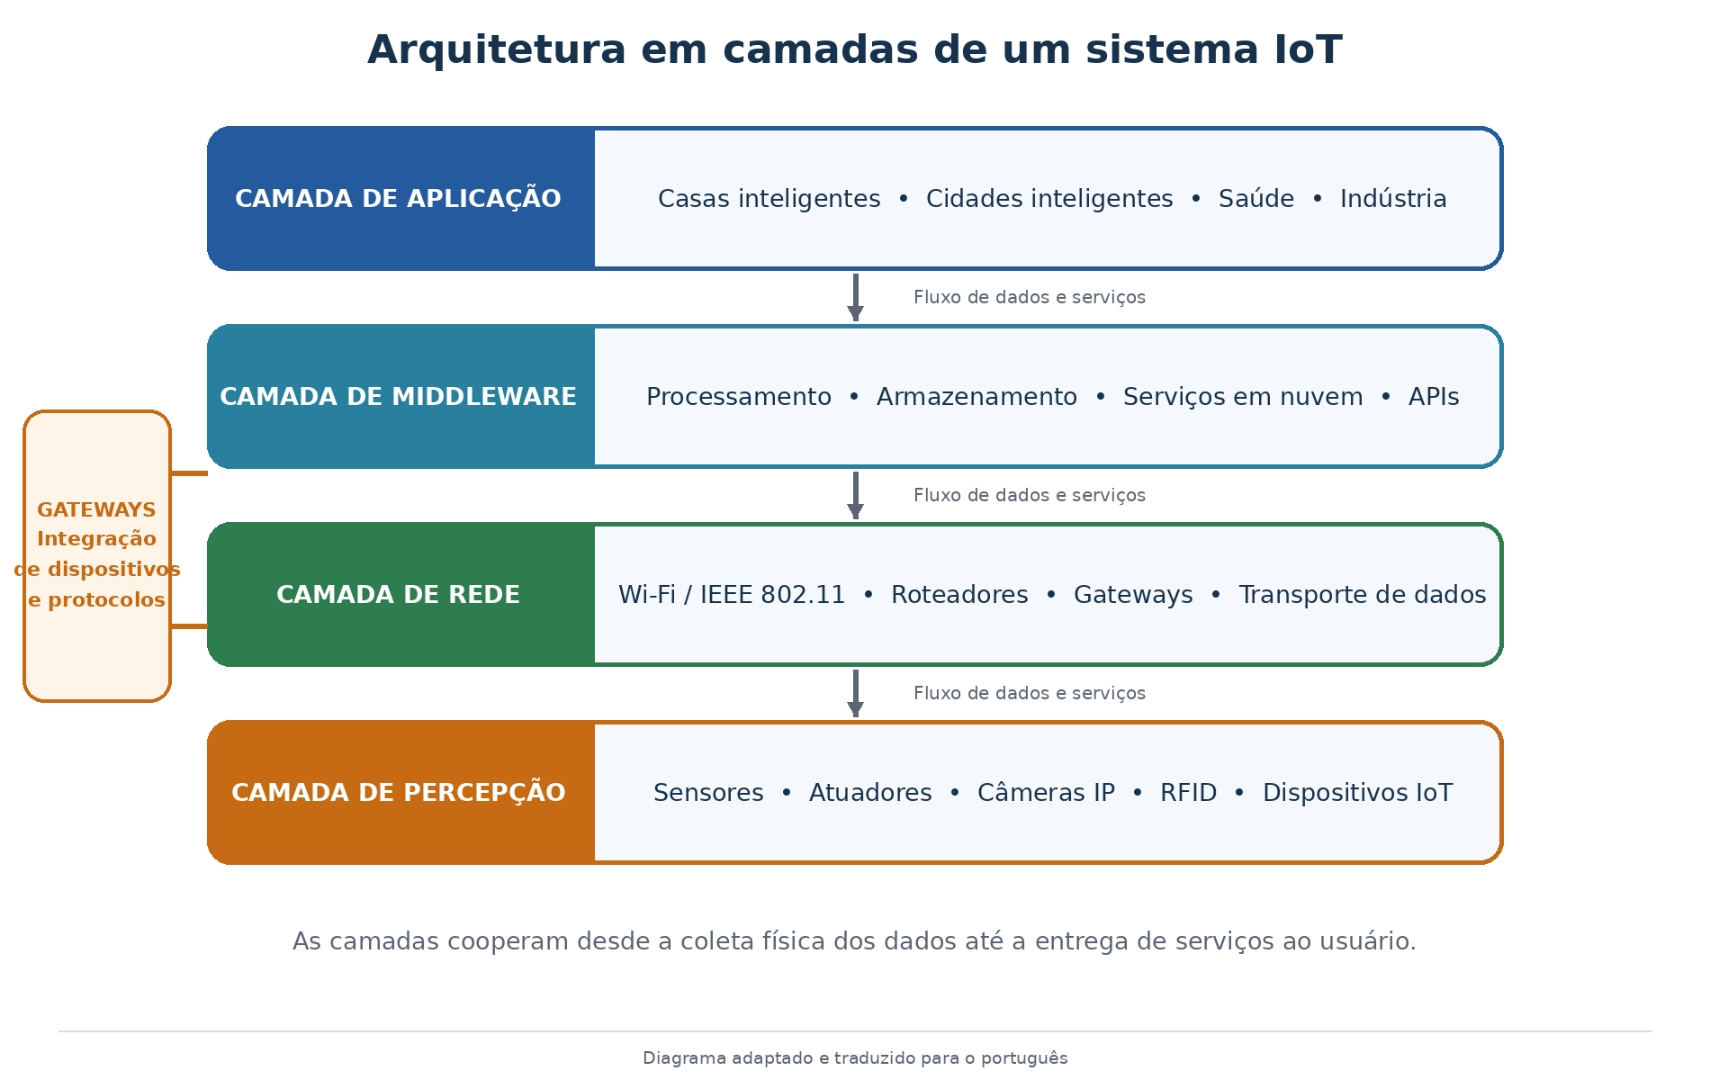
\includegraphics[width=0.98\textwidth]{arquitetura_camadas_iot}
\legend{Fonte: adaptado de Hassija et al. (2019).}
\end{figure}

\subsection{Restrições de hardware e energia}

Para garantir viabilidade comercial, fabricantes de dispositivos IoT frequentemente utilizam processadores de baixa potência, memória restrita e módulos de comunicação simplificados, e muitos equipamentos operam sob limites energéticos severos, empregando técnicas como o \textit{Target Wake Time} (TWT) para permanecer longos períodos em suspensão \cite{FarhadPyun2022}. \citeonline{Yuksel2020} analisou o consumo de energia de um dispositivo IoT baseado em Wi-Fi e a influência do módulo Wi-Fi nesse consumo, sem tratar de ataques. A partir disso, formula-se apenas como hipótese que, sob um ataque contínuo de desautenticação, um dispositivo nessas condições seja forçado a despertar repetidamente para renegociar a associação, elevando o consumo além de ficar indisponível. Essa hipótese não foi testada: o consumo energético não foi medido neste trabalho, cujos dispositivos avaliados são alimentados pela rede elétrica, à exceção do \textit{smartphone}.

\subsection{Atualização de \textit{firmware} e suporte a WPA3 e PMF}

A correção para a fragilidade das tramas de gerenciamento passa pelo uso de PMF, seja com WPA2, seja com WPA3. \citeonline{Lima2025} observa que uma parcela expressiva dos dispositivos inteligentes comercializados, como lâmpadas, interruptores e sensores de presença, utiliza módulos de rádio limitados ao Wi-Fi~4 (IEEE~802.11n), operando apenas na faixa de 2,4~GHz. Essa característica, porém, não impede por si só o uso de WPA3 ou de PMF, pois ambos são mecanismos de segurança da camada MAC, independentes da geração da camada física e da faixa de frequência. O próprio ESP32-S3 é um contraexemplo: seu rádio é IEEE~802.11 b/g/n e opera somente em 2,4~GHz \cite{EspressifS3Datasheet}, e ainda assim a pilha oficial da Espressif oferece suporte a WPA3-\textit{Personal} e a PMF nos modos opcional e obrigatório \cite{EspressifWifiSecurity}. Nos ensaios deste trabalho, a lâmpada inteligente, que também opera em 2,4~GHz, negociou SAE com PMF obrigatório (Apêndice~\ref{sec:evidencias-rsn}).

A barreira, portanto, está menos no rádio e mais no \textit{software}: módulos com \textit{drivers} gravados em \textit{Read-Only Memory} (ROM), pouco espaço para atualizações ou fabricantes que não distribuem novas versões de \textit{firmware} podem deixar de oferecer SAE e PMF mesmo quando o \textit{hardware} os comportaria \cite{Lima2025}. Para preservar a compatibilidade com esses dispositivos, o roteador pode ser configurado em modo de transição WPA2/WPA3, como no cenário misto deste trabalho. Como a negociação ocorre por associação (Seção~\ref{subsec:consolidacao_resultados}), essa escolha não rebaixa a segurança das estações que suportam SAE e PMF, mas mantém expostas à desautenticação forjada as estações que negociam WPA2 sem PMF \cite{Lima2025}.

\subsection{Taxonomia de ameaças em dispositivos de consumo}

O impacto das restrições de \textit{hardware} resulta em um ecossistema frágil sob múltiplas perspectivas. \citeonline{Hassija2019} apresentam uma taxonomia abrangente de ameaças voltada especificamente para a IoT, mapeando vetores de ataque em diferentes camadas da arquitetura. Entre esses vetores, destacam-se ataques de rádio e enlace, como \textit{jamming}, falsificação de identidade, negação de serviço, exploração de mecanismos de autenticação deficientes e interceptação de tráfego \cite{Hassija2019}.

Três conceitos dessa taxonomia precisam ser distinguidos, pois são frequentemente tratados como sinônimos. A \textbf{falsificação de quadros de desautenticação} é um ataque de protocolo: o atacante transmite quadros de gerenciamento válidos em formato, mas com endereço de origem forjado, e só é efetivo contra associações que não negociaram PMF. Na prática, o atacante se passa pelo ponto de acesso: o quadro é enviado com o endereço MAC do ponto de acesso (BSSID) como origem e o endereço da estação-alvo como destino, ou o endereço de difusão, para atingir todas as estações da rede. Como, sem PMF, a estação não tem meios de verificar a autenticidade do quadro, ela o aceita como se tivesse sido enviado pelo próprio ponto de acesso e encerra a associação \cite{KohliosHayajneh2018}. A \textbf{negação de serviço} não é uma técnica, mas uma categoria de efeito, a perda de disponibilidade, que pode ser obtida por diversos meios, entre eles a falsificação de quadros. O \textbf{\textit{jamming}}, por fim, é interferência na camada física: o atacante ocupa ou corrompe o canal de rádio, independentemente do conteúdo dos quadros \cite{Hassija2019,Amoordon2022}. O PMF atua apenas sobre o primeiro caso: garante a integridade e a autenticidade dos quadros de gerenciamento robustos \cite{CiscoMFP2024}, mas não garante disponibilidade. Interferência física, ocupação do canal por grande volume de quadros e ataques a quadros que o PMF não protege, como \textit{beacons}, autenticação e associação, permanecem possíveis mesmo com PMF ativo.

Em ambientes conectados por Wi-Fi, essas ameaças exploram diretamente a dependência da comunicação sem fio. Em vez de comprometer o sigilo dos dados por meio de quebra criptográfica, muitos ataques exploram a lógica de controle e coordenação da rede, impondo indisponibilidade, perda de sincronização e reconexões sucessivas. Em redes IoT de consumo, tais efeitos se traduzem em dispositivos que deixam de atuar conforme o esperado e em perdas de monitoramento em tempo real.

À luz dessa taxonomia, o ataque investigado neste trabalho é a falsificação de quadros de desautenticação, cujo efeito pretendido é a negação de serviço na camada de enlace; ele não envolve \textit{jamming}. Sua particularidade é atingir o elo de borda entre a camada de rede (roteadores Wi-Fi) e a camada de percepção (dispositivos IoT). É a interseção entre limitações de \textit{firmware}, dependência do IEEE~802.11 e associações sem PMF que torna o cenário investigado sensível a ataques simples, porém de alto impacto prático.

A Figura~\ref{fig:taxonomia_ameacas_iot} sintetiza as principais ameaças associadas às camadas de percepção, rede, \textit{middleware} e aplicação. Para este estudo, destacam-se os ataques de interferência e privação de sono na camada de percepção, bem como os ataques de negação de serviço e aos dados em trânsito na camada de rede, pois esses vetores podem comprometer a disponibilidade dos dispositivos conectados por IEEE~802.11 \cite{Hassija2019}.

\begin{figure}[htb]
\centering
\caption{Taxonomia de ameaças de segurança por camada da IoT}
\label{fig:taxonomia_ameacas_iot}
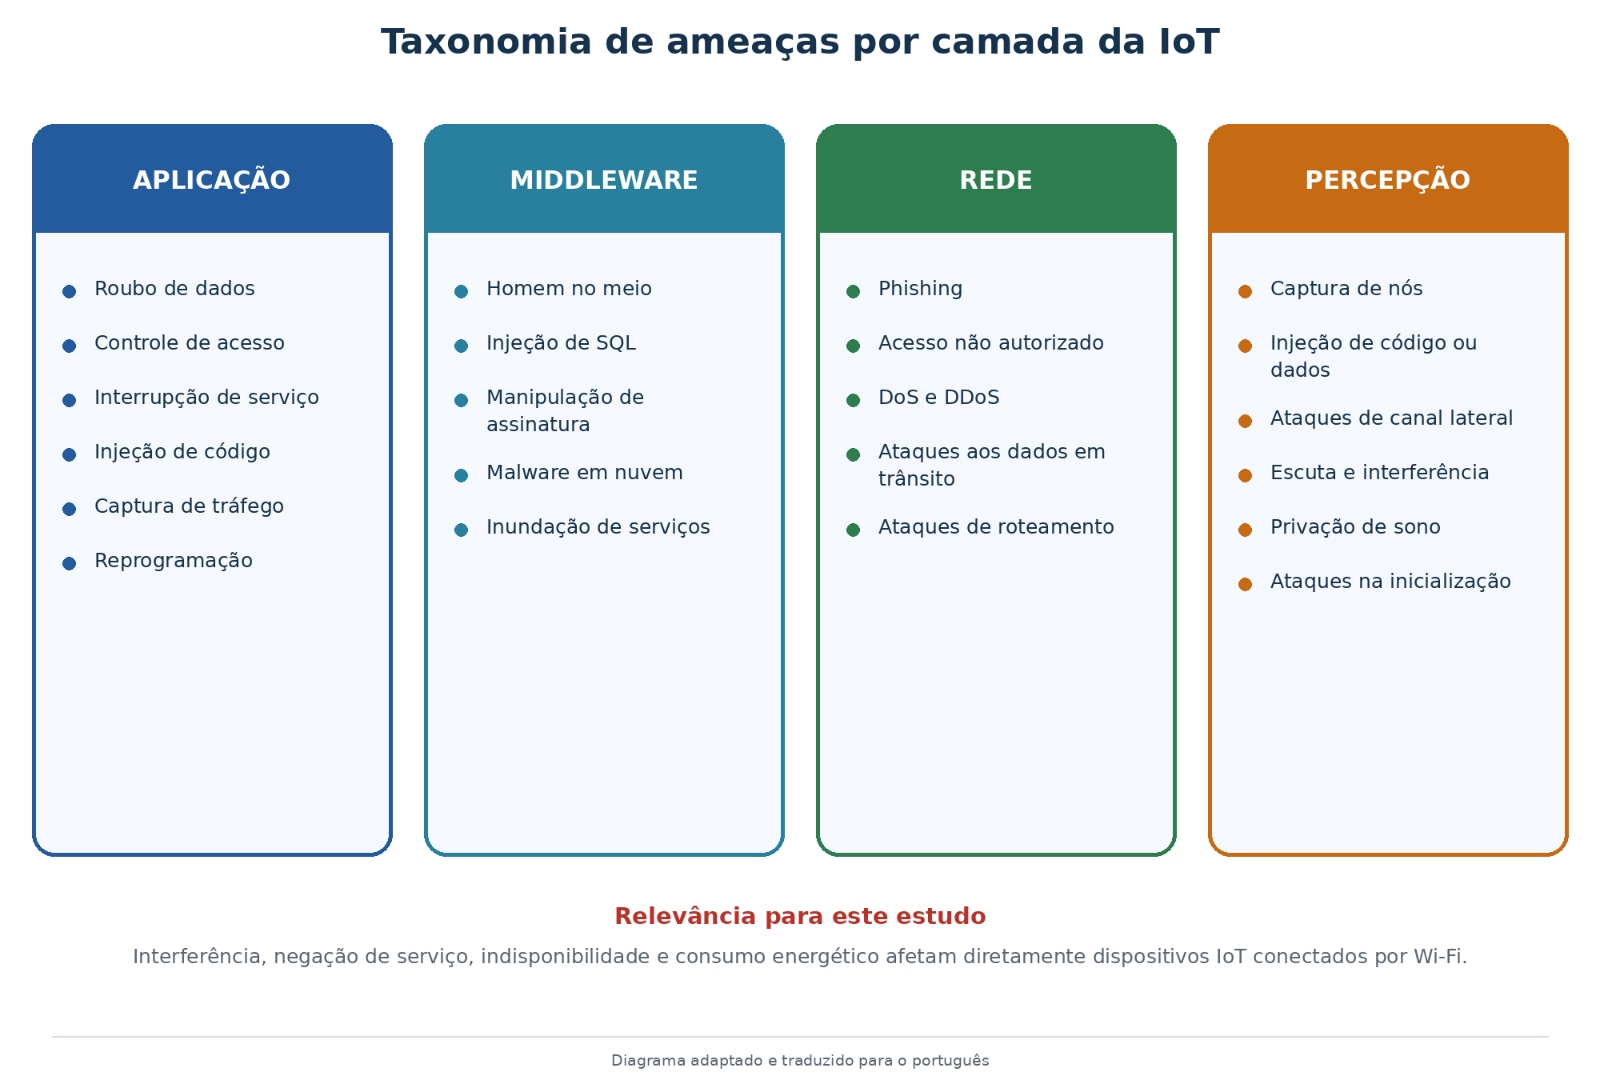
\includegraphics[width=0.98\textwidth]{taxonomia_ameacas_iot}
\legend{Fonte: adaptado de Hassija et al. (2019).}
\end{figure}

\section{Avaliação prática e estado da arte}

\subsection{Ataques combinados: desautenticação e \textit{Evil Twin}}
\label{subsec:evil_twin}

O ataque de desautenticação também é citado como etapa preparatória de intrusões mais sofisticadas, como o \textit{Evil Twin}. \citeonline{Amoordon2022} documentam a ocorrência combinada da criação de pontos de acesso falsos, \textit{jamming} de varredura de frequência e ataques de desautenticação em redes IEEE~802.11.

Nesse ataque, o atacante configura um ponto de acesso falso que replica informações do roteador legítimo, como SSID, BSSID e canal, eventualmente com potência maior, e envia quadros de desautenticação para que a vítima perca a conexão e procure novamente a rede \cite{LitayemAlsadi2023,Amoordon2022}. Copiar o SSID e aumentar a potência, contudo, não garante que o cliente se autentique no clone quando a rede legítima é protegida. No WPA2-PSK, o \textit{4-way handshake} exige que os dois lados demonstrem conhecer a senha: a mensagem~3 do ponto de acesso carrega um MIC calculado com a chave derivada dela, e um ponto de acesso que não a conhece não completa a troca; no WPA3-\textit{Personal}, a troca SAE tem o mesmo efeito \cite{KohliosHayajneh2018}. Assim, a reconexão automática a um clone só se completa se o atacante já conhecer a senha ou se o dispositivo aceitar uma rede com o mesmo nome e segurança diferente (por exemplo, aberta), comportamento que depende da implementação de cada cliente.

Por isso, dois cenários devem ser separados. No primeiro, a \textbf{reconexão automática de um dispositivo IoT}, não há interação humana: sem a senha, o clone não conclui a associação, e o efeito prático do ataque tende a se limitar à indisponibilidade. No segundo, um \textbf{usuário interage com um portal falso}: o atacante oferece uma rede aberta com nome semelhante e um portal cativo que simula a interface do roteador, e a pessoa, motivada pela queda da conexão, é persuadida a digitar a senha da rede \cite{YeboahOforiHawsh2023}. Esse segundo cenário depende de engenharia social, e não de uma falha de autenticação do protocolo, e não se aplica diretamente a dispositivos IoT sem interface para digitar credenciais. Neste trabalho, apenas a etapa de desautenticação foi avaliada.

O encadeamento entre a desautenticação e a criação de um ponto de acesso malicioso é representado na Figura~\ref{fig:ataque_evil_twin}, que deve ser lida com as condições descritas acima.

\begin{figure}[htb]
\centering
\caption{Funcionamento conceitual de um ataque Evil Twin em uma rede sem fio}
\label{fig:ataque_evil_twin}
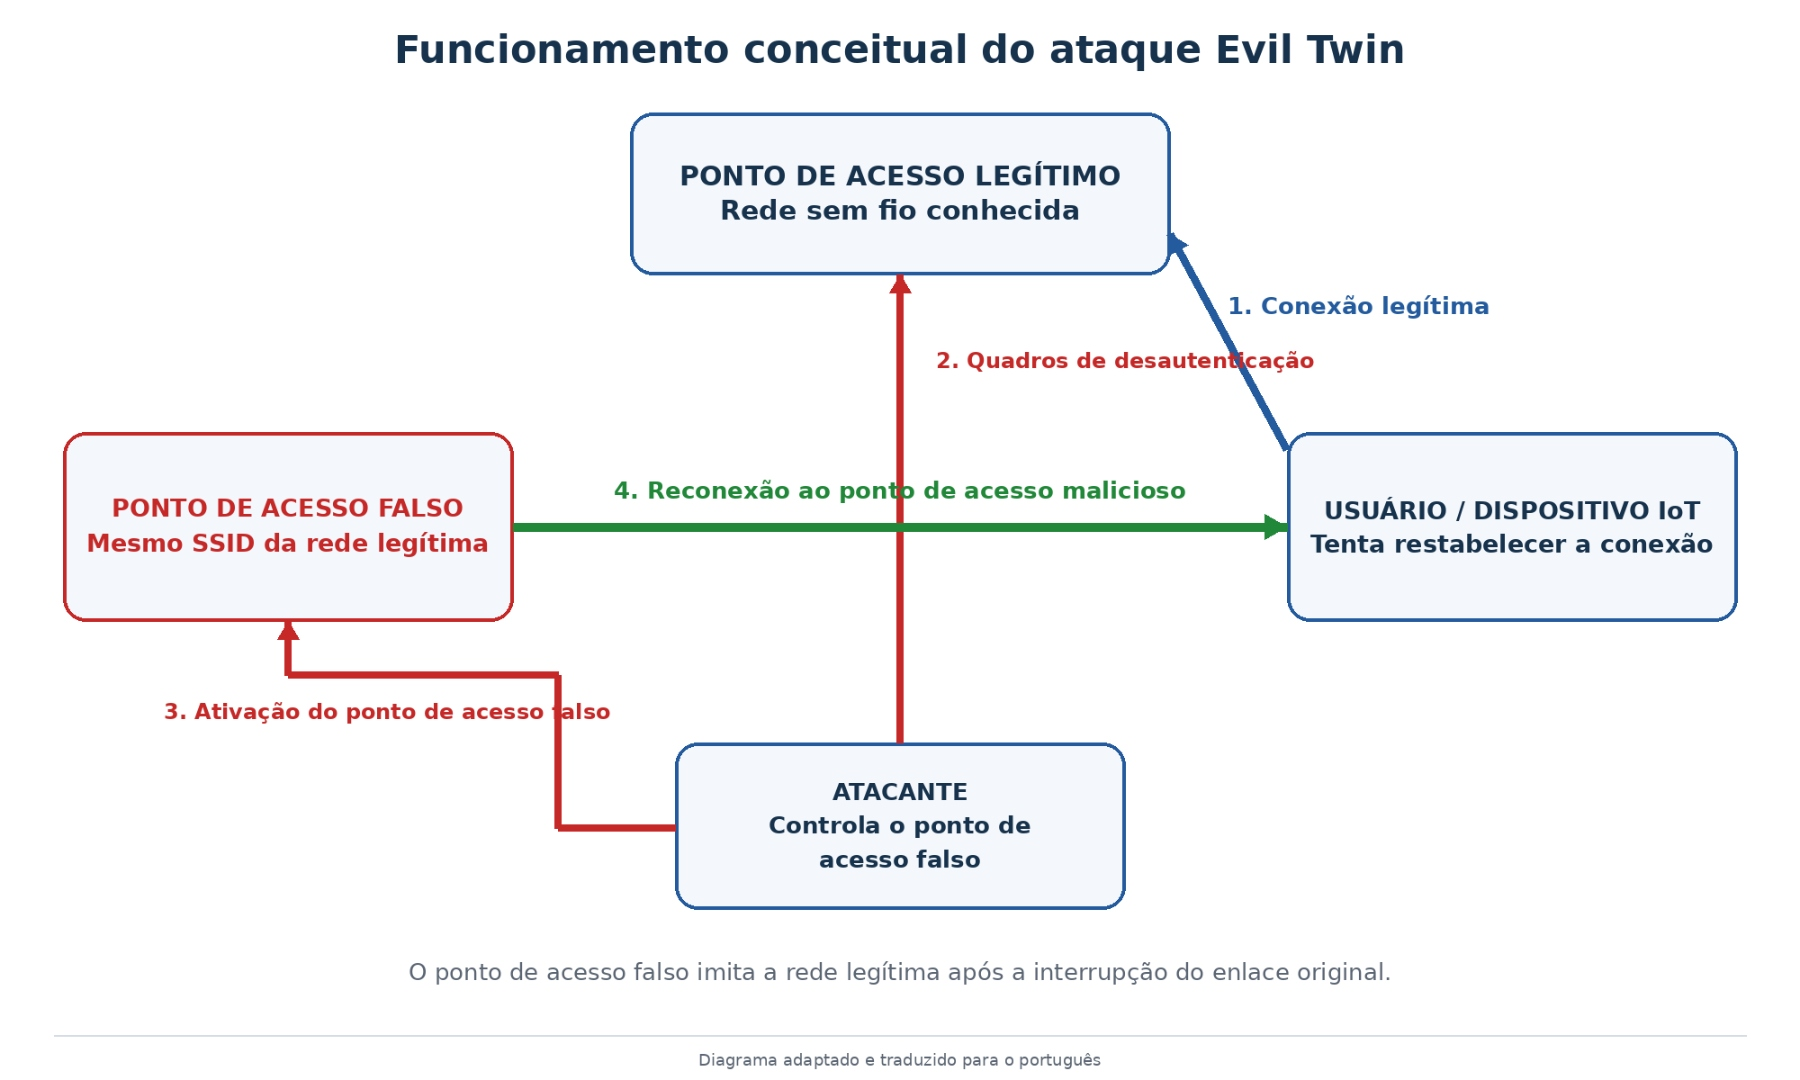
\includegraphics[width=0.98\textwidth]{ataque_evil_twin}
\legend{Fonte: adaptado de Yeboah-Ofori e Hawsh (2023). A captura da vítima pelo ponto de acesso falso pressupõe que o atacante conheça a senha da rede ou que a vítima aceite uma rede aberta e interaja com o portal falso; a cópia do SSID e o aumento de potência não bastam em redes WPA2-PSK ou WPA3-SAE.}
\end{figure}

\subsection{Análise de impacto: o estudo de Kristiyanto e Ernastuti}

\citeonline{KristiyantoErnastuti2020} realizaram um teste de penetração externa utilizando o microcontrolador NodeMCU ESP8266 para atacar a conectividade de uma câmera IP com um roteador Wi-Fi. Para quantificar o impacto, os autores utilizaram \textit{softwares} do tipo \textit{sniffer}, como o CommView, capazes de registrar o tráfego no ar.

A análise demonstrou degradações imediatas na qualidade da rede. Ao ser alvejada por pacotes de desautenticação, a câmera IP perdeu o sinal de vídeo, e os registros técnicos indicaram que o dispositivo tentou mitigar a interferência por meio de saltos de canal. Além disso, os dados de telemetria mostraram queda da taxa de transferência de dados do ambiente e anomalias em elementos de controle da comunicação, como os \textit{retry bits} e o \textit{sequence number}, que sofreram reinicializações inesperadas durante a troca de dados \cite{KristiyantoErnastuti2020}. Esse resultado é coerente com a premissa de que proteger apenas os dados do usuário, sem proteger os quadros de gerenciamento, mantém a disponibilidade dos dispositivos exposta \cite{Lima2025}.

A topologia utilizada por Kristiyanto e Ernastuti (2020) é apresentada na Figura~\ref{fig:topologia_deauth_esp8266}. O cenário reúne um ESP8266 como plataforma de teste, um ponto de acesso e uma câmera IP como dispositivo IoT avaliado, constituindo uma referência experimental diretamente relacionada ao recorte deste trabalho.

\begin{figure}[htb]
\centering
\caption{Topologia experimental de um ataque de desautenticação com ESP8266}
\label{fig:topologia_deauth_esp8266}
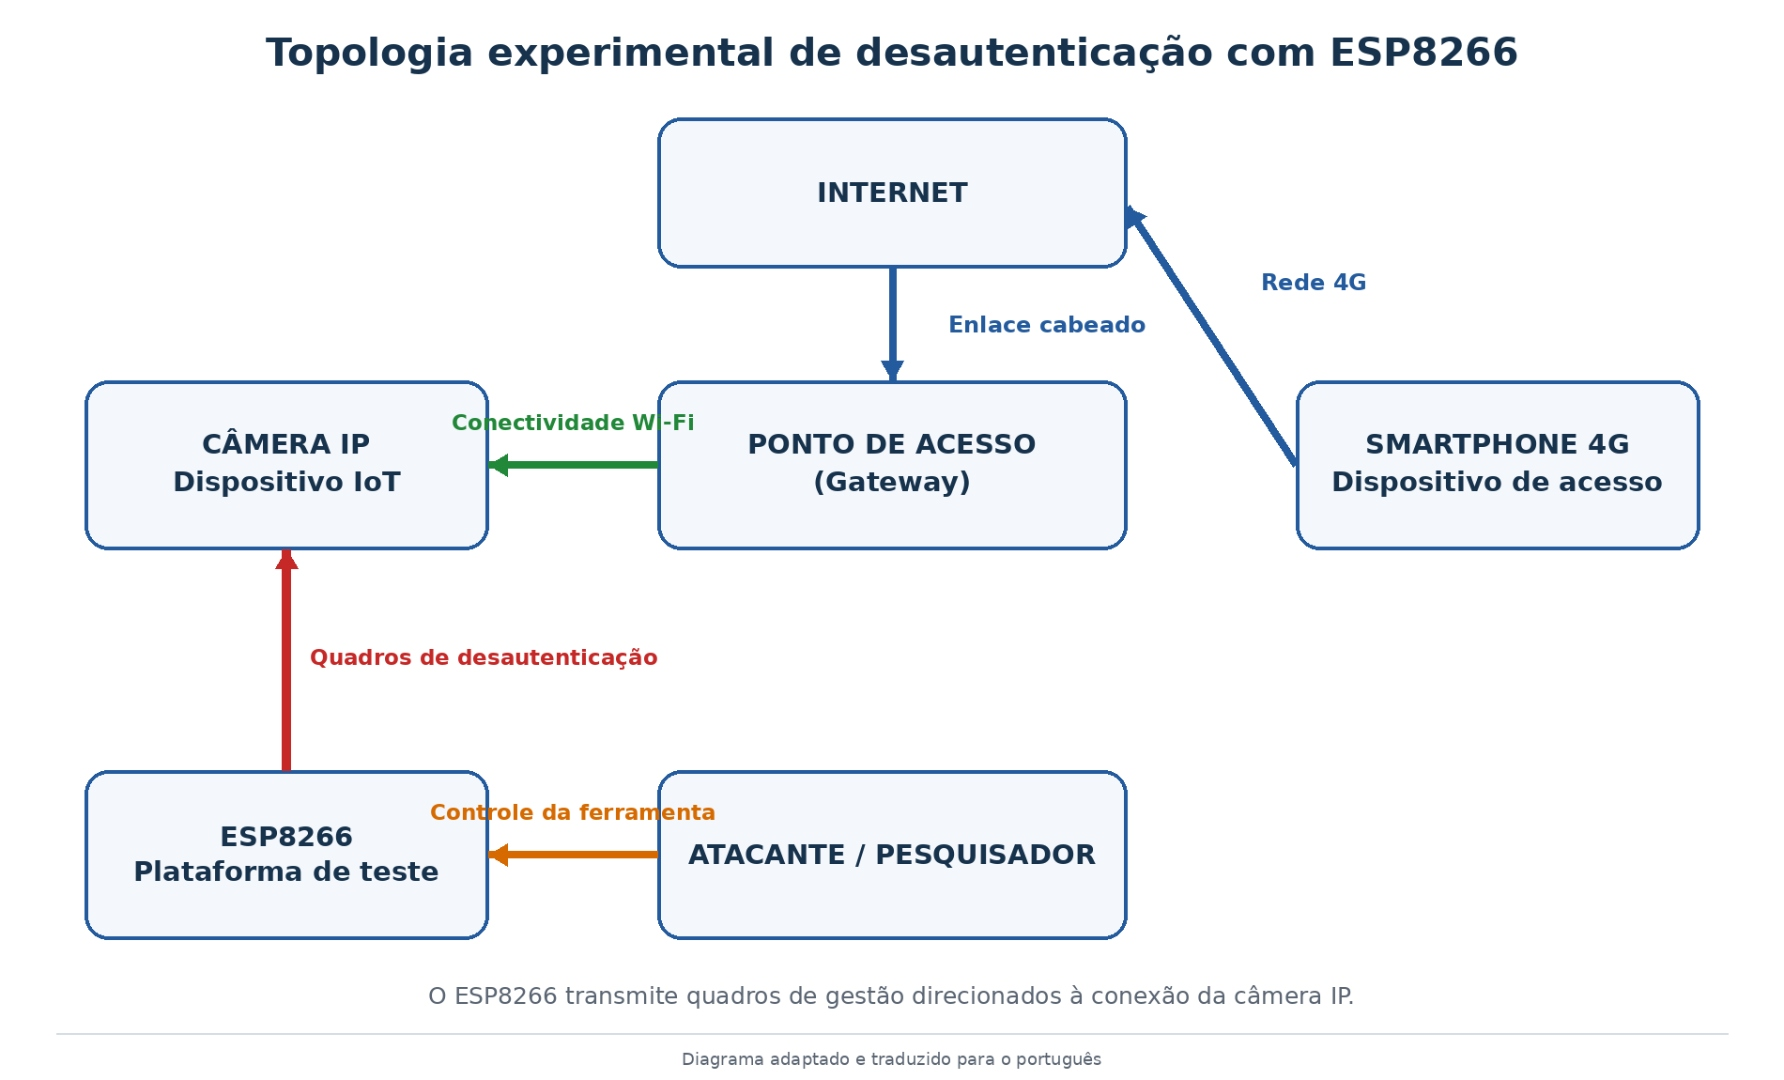
\includegraphics[width=0.94\textwidth]{topologia_deauth_esp8266}
\legend{Fonte: adaptado de Kristiyanto e Ernastuti (2020, p. 48).}
\end{figure}

\section{Trabalhos relacionados}
\label{sec:trabalhos_relacionados}

Esta seção compara este trabalho com os estudos mais próximos do seu recorte. O Quadro~\ref{quad:trabalhos-relacionados} organiza, para cada estudo, o equipamento de ataque ou análise, os dispositivos avaliados, a condição de segurança e de PMF, as métricas, o número de repetições, as limitações e a diferença em relação a este trabalho. Quando o texto original não informa um item, a célula indica ``Não informado''; nenhuma informação foi estimada.

\begin{landscape}
\begin{quadro}[p]
\centering
\caption{Comparação entre trabalhos relacionados e este estudo}
\label{quad:trabalhos-relacionados}
\marcadoresTabela
\scriptsize
\setlength{\tabcolsep}{2.5pt}
\renewcommand{\arraystretch}{1.15}
\begin{tabular}{|>{\raggedright\arraybackslash}p{2.2cm}|>{\raggedright\arraybackslash}p{2.7cm}|>{\raggedright\arraybackslash}p{2.6cm}|>{\raggedright\arraybackslash}p{2.9cm}|>{\raggedright\arraybackslash}p{2.9cm}|>{\raggedright\arraybackslash}p{2.0cm}|>{\raggedright\arraybackslash}p{2.6cm}|>{\raggedright\arraybackslash}p{3.4cm}|}
\hline
\textbf{Autor/ano} & \textbf{Equipamento} & \textbf{Dispositivos} & \textbf{Segurança/PMF} & \textbf{Métricas} & \textbf{Repetições} & \textbf{Limitações} & \textbf{Diferença para este TCC} \\ \hline
\citeonline{KristiyantoErnastuti2020} & NodeMCU ESP8266 (ataque); CommView (captura) & Câmera IP e roteador Wi-Fi & Não informado no texto; o artigo afirma que os quadros de gerenciamento não são criptografados & Perda do vídeo, vazão, \textit{retry bits}, \textit{sequence number}, saltos de canal & Não informado (um cenário descrito) & Um único tipo de dispositivo (câmera IP) & Quatro dispositivos, dois cenários de segurança, AKM e PMF verificados por associação, tempo sem resposta medido por \textit{ping} \\ \hline
\citeonline{Amoordon2022} & \textit{aireplay-ng} (desautenticação); \textit{hostapd} (AP falso); Matlab e gerador de sinal (\textit{jamming}); captura em modo monitor & Computador portátil (cliente) e \textit{Raspberry Pi} (servidor), sem dispositivos IoT & Não informado; 802.11b/n no canal 13 & Desempenho de um modelo supervisionado na detecção de AP falso, \textit{jamming} de varredura e desautenticação (precisão e acurácia) & 1 captura de 2~min por situação & Foco em detecção, não no impacto por dispositivo & Mede o impacto do ataque em cada dispositivo, em vez de detectá-lo \\ \hline
\citeonline{Lima2025} & Aircrack-ng (injeção); Wireshark (captura) & \textit{Hosts} clientes em rede doméstica; IoT discutido, sem modelos avaliados & Redes IEEE~802.11n e 802.11ac sob WPA2 e WPA3; recomenda 802.11w & Interrupção da comunicação e estado dos quadros (avaliação qualitativa) & Não informado & Não quantifica o resultado; IoT apenas discutido, sem dispositivos testados & Uso de plataforma portátil ESP32-S3 (T-Embed, Bruce) em vez de Aircrack-ng em computador; caracterização por dispositivo com evidência RSN \\ \hline
Este trabalho & LILYGO T-Embed CC1101 Plus (ESP32-S3, Bruce 1.16.1); AR9271 em modo monitor e \textit{tshark} & Câmera IP, lâmpada, tomada e \textit{smartphone} & WPA2 sem PMF oferecido; modo misto com PMF opcional; AKM e MFPC/MFPR por associação & Quadros de desautenticação, tempo sem resposta a \textit{ping}, perda de associação & 3 em WPA2 (câmera: 2 com \textit{ping} + piloto); 1 no modo misto (2 para câmera e \textit{smartphone}) & Amostra pequena; sem condição de WPA2 com PMF; apenas 2,4~GHz & --- \\ \hline
\end{tabular}
\legend{Fonte: elaborado pelo autor a partir dos trabalhos citados (2026).}
\end{quadro}
\end{landscape}

O Quadro~\ref{quad:trabalhos-relacionados} mostra que o estudo de \citeonline{KristiyantoErnastuti2020} é o mais próximo do arranjo experimental deste trabalho, por combinar microcontrolador, ponto de acesso e câmera IP, mas se concentra em um único tipo de dispositivo. O trabalho de \citeonline{Amoordon2022} trata do mesmo tipo de ataque sob a perspectiva da detecção, sem caracterizar o impacto em cada dispositivo. Em relação a \citeonline{Lima2025}, que estuda a desautenticação e sua mitigação em redes 802.11n e 802.11ac sob WPA2 e WPA3, com o Aircrack-ng como ferramenta de injeção e o Wireshark para captura, este trabalho acrescenta dois elementos: o uso de uma plataforma de ataque portátil baseada em ESP32-S3, integrada a uma placa portátil (LILYGO T-Embed CC1101 Plus com \textit{firmware} Bruce), e a caracterização do comportamento de cada dispositivo, que relaciona a segurança efetivamente negociada na associação (AKM e bits MFPC/MFPR) ao tempo sem resposta e à perda de associação observados.

Em síntese, os estudos analisados indicam que ataques de desautenticação causam indisponibilidade em redes IEEE~802.11 sem PMF \cite{KristiyantoErnastuti2020,Amoordon2022,Lima2025}, e \citeonline{KristiyantoErnastuti2020} mostram que isso é viável com um ESP8266. A maior parte desses trabalhos, porém, concentra-se em um único tipo de dispositivo ou em modelos de detecção, deixando pouco explorado, de forma sistemática, o comportamento de diferentes dispositivos IoT de consumo sob ataques gerados por microcontroladores da família ESP em ambiente controlado, com a segurança negociada por cada um verificada nos próprios quadros. É essa lacuna que o estudo de caso proposto busca endereçar.

% !TeX encoding = UTF-8
\chapter{Metodologia}
\label{cap:metodologia}

Este capítulo apresenta os procedimentos metodológicos adotados na pesquisa intitulada ``Vulnerabilidades do IEEE 802.11 em ambientes IoT: estudo de caso utilizando microcontroladores de baixo custo''. São descritas a abordagem, a tipologia, os instrumentos de coleta, o cenário empírico e as técnicas de análise efetivamente empregados.

Trata-se de uma pesquisa aplicada, de abordagem mista (quantitativa e qualitativa), com objetivos exploratórios e descritivos, conduzida como estudo de caso experimental em ambiente laboratorial controlado de rede IEEE 802.11 com dispositivos IoT. A classificação apoia-se nas noções de pesquisa aplicada, exploratória, descritiva, experimental, bibliográfica e documental apresentadas por \citeonline{ProdanovFreitas2013} e \citeonline{Gil2002}.

% ----------------------------------------------------------
% 3.1 Tipo de Pesquisa
% ----------------------------------------------------------
\section{Tipo de pesquisa}

\subsection{Natureza da pesquisa}

A pesquisa é aplicada porque produz conhecimento voltado a um problema prático de segurança de redes sem fio: verificar, em laboratório, como dispositivos IoT selecionados reagem a ataques de desautenticação gerados por um microcontrolador de baixo custo. É exploratória porque examina a interação entre o padrão IEEE 802.11, a segurança negociada (WPA2, WPA3 e PMF) e o comportamento desses dispositivos em um ambiente específico; e é descritiva porque registra de forma sistemática a configuração do ambiente, as características dos dispositivos, os eventos de perda e retomada de conectividade e as métricas observadas, sem pretender construir modelos causais generalizáveis.

Quanto ao recorte temporal, a pesquisa é transversal: os dados foram coletados em um período delimitado, com um ensaio piloto em 3 de novembro de 2026, o conjunto completo de ensaios em 8 de novembro de 2026 e, em 17 de novembro de 2026, seis capturas da câmera em WPA2 (\texttt{R03} e \texttt{R04}, válidas com \textit{ping}; \texttt{R05} e \texttt{R06}, invalidadas; \texttt{R07}, teste de bancada; \texttt{R08}, descritiva; Apêndice~\ref{sec:registro-execucoes}), sem acompanhamento longitudinal dos equipamentos \cite{ProdanovFreitas2013,Gil2002}.

A Figura~\ref{fig:classificacao_pesquisa} sintetiza a classificação metodológica adotada, relacionando a natureza, os objetivos, a abordagem, o procedimento técnico e o recorte temporal da pesquisa.

\begin{figure}[htb]
\centering
\caption{Classificação metodológica da pesquisa}
\label{fig:classificacao_pesquisa}
\resizebox{\textwidth}{!}{%
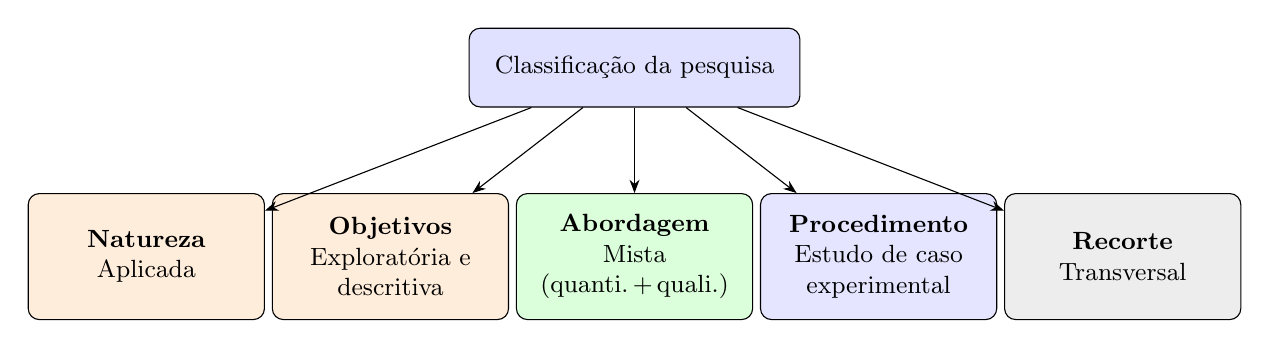
\begin{tikzpicture}[font=\small, >=Stealth,
  c/.style={draw, rounded corners, minimum width=30mm, minimum height=16mm, align=center}]
\node[c, fill=blue!12, minimum height=10mm, minimum width=42mm] (root) at (0,2) {Classificação da pesquisa};
\node[c, fill=orange!14] (nat) at (-6.2,-0.4) {\textbf{Natureza}\\Aplicada};
\node[c, fill=orange!14] (obj) at (-3.1,-0.4) {\textbf{Objetivos}\\Exploratória e\\descritiva};
\node[c, fill=green!14] (abo) at (0,-0.4) {\textbf{Abordagem}\\Mista\\(quanti.\,+\,quali.)};
\node[c, fill=blue!10] (pro) at (3.1,-0.4) {\textbf{Procedimento}\\Estudo de caso\\experimental};
\node[c, fill=gray!14] (tmp) at (6.2,-0.4) {\textbf{Recorte}\\Transversal};
\draw[->] (root) -- (nat);
\draw[->] (root) -- (obj);
\draw[->] (root) -- (abo);
\draw[->] (root) -- (pro);
\draw[->] (root) -- (tmp);
\end{tikzpicture}}
\legend{Fonte: elaborado pelo autor com base em Prodanov e Freitas (2013) e Gil (2002).}
\end{figure}

\subsection{Declaração de uso de inteligência artificial generativa}
\label{subsec:declaracao_ia}

Como o Centro Universitário Dinâmica das Cataratas (UDC) não dispõe de norma institucional específica sobre o tema, toma-se como referência o art.~9º, inciso~I, alíneas~c, d e~f, da Portaria nº 2.664 do Conselho Nacional de Desenvolvimento Científico e Tecnológico (CNPq), de 6 de março de 2026 (CNPq, \citeyear{CNPqPortaria2664}), que orienta declarar a ferramenta de inteligência artificial generativa utilizada e a sua finalidade, em qualquer fase da pesquisa, e atribui aos autores a responsabilidade integral pelo conteúdo final, declara-se o emprego das seguintes ferramentas de inteligência artificial generativa neste trabalho, utilizadas como apoio e sob revisão e validação integral do autor:

\begin{itemize}
    \item \textbf{Perplexity (plano Pro) e GPT-5.4 (OpenAI), utilizados no segundo semestre de 2026:} organização de ideias, apoio à estruturação do texto, revisão linguística e esclarecimento conceitual a partir de referências selecionadas pelo autor;
    \item \textbf{Claude (Anthropic, plano Claude Pro), com os modelos Claude Opus 5.5 e Claude Opus 4.8 no Claude Code (extensão do VS Code) e Claude Opus 5.5 no aplicativo \textit{desktop}, utilizado no segundo semestre de 2026:} revisão técnica e linguística do texto; redação de versões de seções a partir das instruções e dos dados fornecidos pelo autor, incluindo a reescrita dos capítulos de referencial, metodologia, desenvolvimento e resultados, a conclusão e o resumo; apoio à extração automatizada de campos dos arquivos de captura com o \textit{tshark} (contagens de quadros e campos do elemento RSN); elaboração dos \textit{scripts} de cálculo das métricas de \textit{ping} (\texttt{src/analisa\_ping.py}) e de geração das Figuras~\ref{fig:comparacao_pmf} e~\ref{fig:ping_lampada} (\texttt{src/figura\_comparacao\_pmf.py} e \texttt{src/figura\_ping\_lampada.py}), revisados e executados pelo autor; e conferência de metadados das referências.
\end{itemize}

Nenhum dado experimental foi gerado pelas ferramentas: todos os valores apresentados provêm dos arquivos de captura e dos \textit{logs} de \textit{ping} produzidos pelo autor nos ensaios, e nenhum valor foi estimado. O autor revisou todo o conteúdo produzido com apoio das ferramentas, conferiu as referências e assume integral responsabilidade pela originalidade, pela precisão das informações e pelas conclusões apresentadas.

Os \textit{scripts} de análise (\texttt{src/analisa\_ping.py}, \texttt{src/figura\_comparacao\_pmf.py} e \texttt{src/figura\_ping\_lampada.py}), o \textit{script} de coleta, os \textit{logs} de \textit{ping} e versões filtradas dos arquivos de captura estão disponíveis no repositório público indicado ao final deste trabalho, depois dos apêndices. As versões filtradas mantêm apenas os quadros da rede de laboratório, sem os quadros do \textit{handshake} de autenticação e sem os quadros de redes vizinhas, e preservam todos os quadros usados nas análises. Os arquivos de captura originais foram entregues ao orientador em mídia digital junto com a versão final deste trabalho.

\subsection{Abordagem metodológica}

Segundo \citeonline{ProdanovFreitas2013}, abordagens quantitativas fundamentam-se na mensuração de variáveis, enquanto abordagens qualitativas buscam compreender significados e relações presentes nos fenômenos estudados; a abordagem mista combina, de forma planejada, os dois tipos de procedimento.

Neste estudo, a abordagem foi mista, com predominância quantitativa. A dimensão quantitativa compreendeu métricas extraídas das capturas e dos registros de conectividade: número de quadros de desautenticação direcionados a cada dispositivo, tempo acumulado sem resposta a \textit{ping}, maior intervalo contínuo sem resposta e ocorrência de novas autenticações e associações. Essas métricas foram comparadas entre dispositivos e entre as duas configurações de segurança do ponto de acesso (WPA2 e modo misto WPA2/WPA3).

A dimensão qualitativa compreendeu a interpretação técnica dos eventos: a forma como o ataque se manifestou nos quadros de gerenciamento, a segurança negociada por cada dispositivo (elemento RSN dos quadros de associação), o modo de recuperação de cada equipamento (automática, intermitente ou dependente de intervenção manual) e as limitações da plataforma de baixo custo.

\subsection{Procedimentos técnicos}

A pesquisa foi operacionalizada como estudo de caso experimental em uma bancada que reproduz, em pequena escala, uma rede doméstica com dispositivos IoT. O conjunto de equipamentos foi composto por roteador TP\mbox{-}Link EX1500, plataforma LILYGO T\mbox{-}Embed CC1101 Plus (baseada em ESP32\mbox{-}S3, \textit{firmware} Bruce 1.16.1), câmera IP, lâmpada inteligente, tomada inteligente e \textit{smartphone} Android, cuja descrição completa consta da Seção~\ref{sec:inventario}.

% ----------------------------------------------------------
% 3.2 Procedimentos Metodológicos
% ----------------------------------------------------------
\section{Procedimentos metodológicos}

O cenário empírico foi uma rede Wi-Fi própria, criada exclusivamente para a pesquisa (TCC\_LAB, 2,4~GHz, canal 6), centrada no roteador TP\mbox{-}Link EX1500, que atuou como ponto de acesso nas duas configurações de segurança avaliadas. O ataque foi gerado pelo LILYGO T\mbox{-}Embed CC1101 Plus, e a captura de quadros IEEE~802.11 foi feita por um adaptador Wi-Fi \textit{Universal Serial Bus} (USB) em modo monitor, conectado a uma máquina virtual com Kali Linux. Os dispositivos avaliados foram uma câmera IP, uma lâmpada inteligente, uma tomada inteligente e um \textit{smartphone} Android de referência.

Do ponto de vista ético e de proteção de dados, todos os testes foram
realizados exclusivamente na rede própria, sem utilização de redes de
terceiros e sem coleta de dados pessoais. Não foram armazenadas
informações sensíveis, como credenciais reais, conteúdos privados de
comunicação ou dados que permitam a identificação de pessoas físicas;
a análise limitou-se a quadros de controle e gerenciamento e a registros
de conectividade em ambiente controlado, em conformidade com os princípios
da Lei Geral de Proteção de Dados (Lei nº 13.709/2018).

Os sujeitos de pesquisa foram os próprios dispositivos e elementos de infraestrutura do ambiente experimental, sem participação de seres humanos. A amostra foi não probabilística e intencional, definida por conveniência a partir dos equipamentos disponíveis.

\subsection{Métodos de coleta de informações}

Foram utilizados instrumentos bibliográficos, documentais e empíricos. A pesquisa bibliográfica reuniu o conhecimento sobre segurança em redes IEEE 802.11, vulnerabilidades em tramas de gerenciamento, ataques de desautenticação, uso de microcontroladores da família ESP em testes de segurança e riscos em ambientes IoT. A pesquisa documental abrangeu manuais e documentações técnicas dos equipamentos e ferramentas, como o \textit{datasheet} do ESP32-S3, a documentação de segurança Wi-Fi da Espressif e a documentação de PMF da Cisco.

No plano empírico, cada ensaio produziu dois registros gerados simultaneamente na estação de captura: um arquivo de captura de quadros IEEE~802.11 em modo monitor (gravado pelo Wireshark/\textit{dumpcap} no ensaio piloto e pelo \textit{tcpdump}, acionado por um \textit{script} auxiliar, nos demais ensaios) e um registro de conectividade por \textit{ping} com marcas de tempo. Complementarmente, o comportamento visível dos dispositivos (imagem da câmera, estado no aplicativo, mensagens do \textit{smartphone}) foi observado diretamente. Registros gerados pelo \textit{firmware} Bruce não foram utilizados na análise. A cadeia completa de processamento desses dados é descrita na Seção~\ref{sec:dados_captura}.

O encadeamento entre os instrumentos de coleta e a etapa de análise é apresentado na Figura~\ref{fig:fluxo_instrumentos}. A pesquisa bibliográfica e a documental fundamentaram a coleta empírica em laboratório, cujos registros alimentaram a análise mista (quantitativa descritiva e qualitativa de conteúdo).

\begin{figure}[htb]
\centering
\caption{Instrumentos de coleta e etapa de análise da pesquisa}
\label{fig:fluxo_instrumentos}
\resizebox{\textwidth}{!}{%
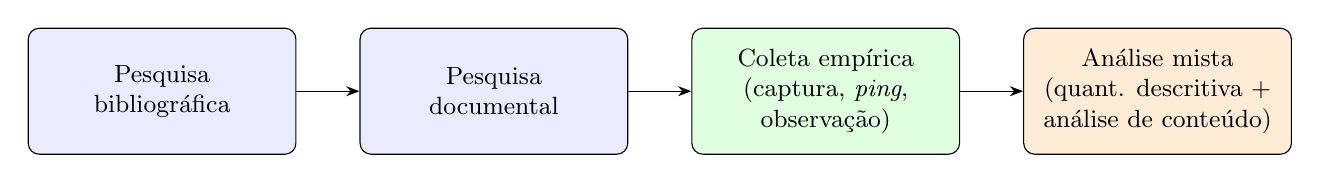
\begin{tikzpicture}[font=\small, >=Stealth,
  p/.style={draw, rounded corners, minimum width=34mm, minimum height=16mm, align=center}]
\node[p, fill=blue!8] (bib) {Pesquisa\\bibliográfica};
\node[p, fill=blue!8, right=8mm of bib] (doc) {Pesquisa\\documental};
\node[p, fill=green!12, right=8mm of doc] (emp) {Coleta empírica\\(captura, \textit{ping},\\observação)};
\node[p, fill=orange!16, right=8mm of emp] (ana) {Análise mista\\(quant. descritiva +\\análise de conteúdo)};
\draw[->] (bib) -- (doc);
\draw[->] (doc) -- (emp);
\draw[->] (emp) -- (ana);
\end{tikzpicture}}
\legend{Fonte: elaborado pelo autor com base em Prodanov e Freitas (2013).}
\end{figure}

\subsection{Métodos de análise das informações}

Na vertente quantitativa, os arquivos de captura foram analisados com o Wireshark, para inspeção visual, e com o \textit{tshark}, para a extração reprodutível de contagens, instantes e campos dos quadros; os \textit{logs} de \textit{ping} foram processados separadamente, e deles derivaram os indicadores de conectividade. Os resultados foram organizados em tabelas por dispositivo e por configuração de segurança, com média e amplitude quando havia mais de uma execução e com o valor observado quando havia uma única execução.

Estava prevista a repetição de cada combinação de dispositivo e configuração em pelo menos três execuções independentes. Esse número foi atingido no cenário WPA2 para a tomada, a lâmpada e o \textit{smartphone}; a câmera, que exigia reinício manual a cada ensaio, teve duas execuções válidas com \textit{ping} em WPA2 (\texttt{CAM\_WPA2\_R03} e \texttt{CAM\_WPA2\_R04}), além do ensaio piloto, sem \textit{ping}; no modo misto, foi realizada uma execução para a tomada e para a lâmpada e duas para a câmera e para o \textit{smartphone} (neste, de três capturas, uma foi invalidada). Em vez de uma classificação binária entre ataque ``bem-sucedido'' e ``não bem-sucedido'', cada execução foi enquadrada em um de quatro resultados, definidos a partir das evidências efetivamente disponíveis. Essa graduação evita atribuir ao ataque um efeito que as evidências não sustentam, já que a falha de respostas a \textit{ping}, isoladamente, não comprova que o dispositivo foi desassociado do ponto de acesso:

\begin{enumerate}
    \item \textbf{Perda de conectividade observada:} durante ou logo após a janela de ataque, o \textit{log} de \textit{ping} registra ao menos um intervalo sem resposta superior ao limiar definido, e a captura contém quadros de desautenticação direcionados ao dispositivo (ou em difusão) na mesma janela. Esse resultado não afirma, por si só, que houve desassociação.
    \item \textbf{Desassociação confirmada:} além da perda de conectividade, a captura mostra evidência de troca de estado na camada de enlace, como a interrupção do tráfego de dados do dispositivo seguida de quadros de autenticação/associação (reassociação) ou o anúncio, no painel do roteador, da saída do cliente.
    \item \textbf{Sem efeito detectado:} há quadros de desautenticação direcionados ao dispositivo na janela de ataque, mas o \textit{log} de \textit{ping} não registra intervalo sem resposta acima do limiar, e o tráfego do dispositivo segue presente na captura.
    \item \textbf{Inconclusivo:} faltam evidências para enquadrar a execução nos casos anteriores, por exemplo, ausência de quadros de desautenticação direcionados ao alvo na janela, \textit{log} de \textit{ping} incompleto ou corrompido, ou falhas de conectividade que não coincidem temporalmente com o ataque.
\end{enumerate}

O tempo entre a queda e o restabelecimento foi registrado sempre que observado, mas não é condição para a classificação: quando o dispositivo não se recuperou até o fim da janela de observação, o tempo é registrado como limite inferior (``pelo menos $X$~s, recuperação espontânea não observada''). Todas as execuções analisadas, inclusive as sem efeito ou inconclusivas, foram mantidas nos registros. A Figura~\ref{fig:criterios_sucesso} representa a sequência de decisão que leva a cada um desses quatro resultados.

\begin{figure}[htb]
\centering
\caption{Classificação do resultado de cada execução do ataque}
\label{fig:criterios_sucesso}
\resizebox{\textwidth}{!}{%
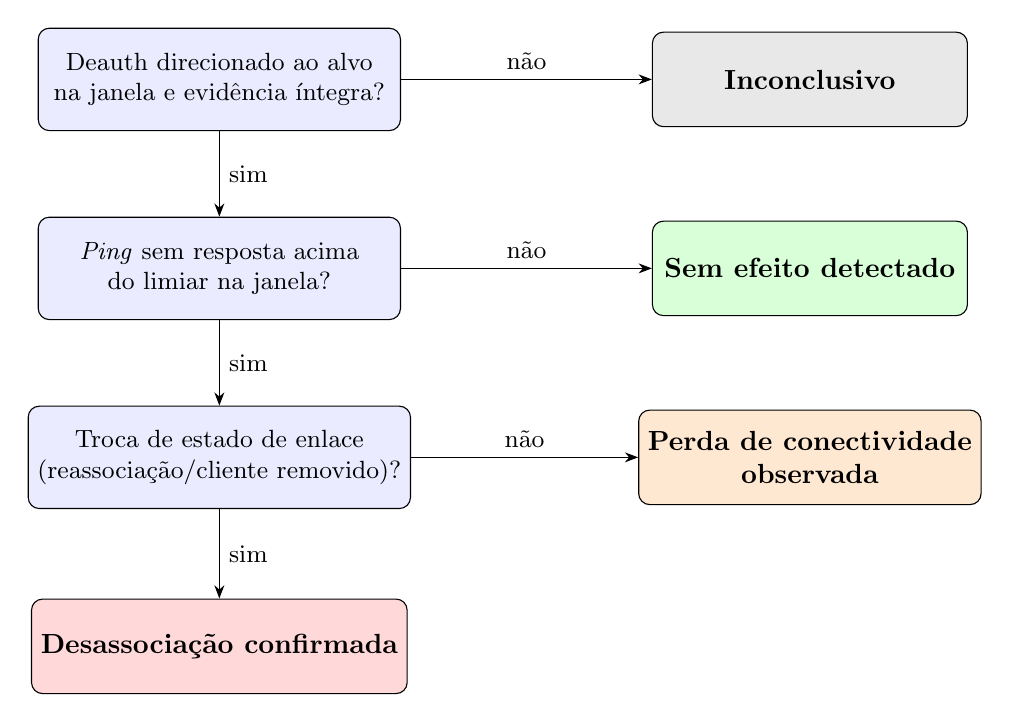
\begin{tikzpicture}[font=\small, >=Stealth,
  q/.style={draw, rounded corners, fill=blue!8, minimum width=46mm, minimum height=13mm, align=center},
  r/.style={draw, rounded corners, minimum width=40mm, minimum height=12mm, align=center, font=\bfseries}]
\node[q] (q1) at (0,3) {Deauth direcionado ao alvo\\na janela e evidência íntegra?};
\node[q] (q2) at (0,0.6) {\textit{Ping} sem resposta acima\\do limiar na janela?};
\node[q] (q3) at (0,-1.8) {Troca de estado de enlace\\(reassociação/cliente removido)?};
\node[r, fill=gray!18] (inc) at (7.5,3) {Inconclusivo};
\node[r, fill=green!15] (sem) at (7.5,0.6) {Sem efeito detectado};
\node[r, fill=orange!18] (perda) at (7.5,-1.8) {Perda de conectividade\\observada};
\node[r, fill=red!15] (des) at (0,-4.2) {Desassociação confirmada};
\draw[->] (q1) -- node[above] {não} (inc);
\draw[->] (q1) -- node[right] {sim} (q2);
\draw[->] (q2) -- node[above] {não} (sem);
\draw[->] (q2) -- node[right] {sim} (q3);
\draw[->] (q3) -- node[above] {não} (perda);
\draw[->] (q3) -- node[right] {sim} (des);
\end{tikzpicture}}
\legend{Fonte: elaborado pelo autor (2026).}
\end{figure}

O monitoramento por \textit{ping} foi feito a partir da estação de captura, diretamente para o endereço IP do dispositivo avaliado, com intervalo de 0,5~s (1~s na primeira execução da tomada em WPA2) e marcas de tempo absolutas em cada resposta. Na vertente qualitativa, empregou-se análise de conteúdo sobre trechos das capturas e sobre o comportamento observado dos dispositivos, para compreender como o ataque se manifestou nas mensagens de protocolo e na função de cada equipamento.

% ----------------------------------------------------------
% Quadro-síntese do delineamento metodológico
% ----------------------------------------------------------
\section{Quadro-síntese do delineamento metodológico}

O Quadro~\ref{quad:delineamento-metodologico} sintetiza, para cada objetivo, as fontes de dados e as técnicas de coleta e análise efetivamente empregadas.

\begin{quadro}[!htbp]
    \centering
    \caption{Delineamento metodológico por objetivo}
    \label{quad:delineamento-metodologico}
    \small
    \renewcommand{\arraystretch}{1.15}
    \begin{tabular}{|p{0.27\textwidth}|p{0.31\textwidth}|p{0.33\textwidth}|}
        \hline
        \textbf{Objetivo} & \textbf{Fonte dos dados} & \textbf{Coleta e análise} \\ \hline
        Geral: analisar e demonstrar as vulnerabilidades do IEEE~802.11 em dispositivos IoT com microcontrolador de baixo custo & Bancada de laboratório (Seção~\ref{sec:inventario}) & Experimento controlado; estatística descritiva e análise de conteúdo \\ \hline
        1. Configurar o ambiente de ataque & Painel do roteador; \textit{firmware} Bruce; documentação técnica & Pesquisa documental; verificação funcional (ensaio piloto) \\ \hline
        2. Executar testes de desautenticação & Capturas \texttt{.pcapng} em modo monitor & Contagem de quadros de desautenticação por dispositivo (\textit{tshark}) \\ \hline
        3. Mensurar indisponibilidade e reconexão & \textit{Logs} de \textit{ping} com marcas de tempo; capturas & Tempo acumulado sem resposta e maior queda contínua; média e amplitude \\ \hline
        4. Analisar o tráfego e documentar as falhas & Quadros de autenticação, associação e desautenticação & Inspeção do elemento RSN (AKM, MFPC/MFPR); comparação com o referencial \\ \hline
    \end{tabular}
    \legend{Fonte: elaborado pelo autor (2026).}
\end{quadro}

O Quadro~\ref{quad:delineamento-metodologico} mostra que os objetivos 2 a 4 se apoiam nas mesmas duas fontes empíricas, as capturas e os \textit{logs} de \textit{ping}, analisadas por técnicas diferentes: contagem de quadros, medição de intervalos sem resposta e inspeção dos campos de segurança. A descrição detalhada dessas fontes e de como foram processadas consta do Capítulo~\ref{cap:desenvolvimento}.

\chapter{Desenvolvimento do Ambiente Experimental}
\label{cap:desenvolvimento}

\section{Visão geral do ambiente experimental}
\label{sec:visao_geral_ambiente}
\label{subsec:adequacao_tipo_projeto}

O produto deste trabalho é um ambiente laboratorial controlado, e não um sistema de informação: não há aplicação, banco de dados ou interface própria, e por isso não foram elaborados diagramas de classes, de sequência ou modelos entidade-relacionamento. A documentação do desenvolvimento concentra-se na configuração da rede, na integração dos componentes, na organização das evidências e nos critérios de validação, representados por um diagrama de blocos (arquitetura) e um fluxograma (sequência dos ensaios).

O ambiente foi composto por um ponto de acesso Wi-Fi, uma plataforma de ataque LILYGO T-Embed CC1101 Plus (ESP32-S3, \textit{firmware} Bruce 1.16.1), três dispositivos IoT comerciais, um \textit{smartphone} de referência e uma estação de captura formada por um \textit{notebook} com Kali Linux em máquina virtual e um adaptador Wi-Fi em modo monitor. Esse conjunto foi usado para executar os ensaios de desautenticação, registrar os quadros IEEE~802.11 e medir o tempo sem resposta de cada dispositivo. O ponto de acesso foi operado em duas configurações de segurança (WPA2 e modo misto WPA2/WPA3), e a segurança efetivamente negociada por cada dispositivo foi verificada nos quadros de associação (Apêndice~\ref{sec:evidencias-rsn}).

\section{Requisitos e regras experimentais}
\label{sec:requisitos_experimento}

Os requisitos foram definidos a partir da fundamentação sobre quadros de gerenciamento do IEEE~802.11 \cite{KohliosHayajneh2018,Amoordon2022}, das características das plataformas ESP \cite{LitayemAlsadi2023} e dos procedimentos da metodologia. Para cada requisito, indica-se como foi atendido.

\subsection{Requisitos funcionais}
\label{subsec:requisitos_funcionais}

\begin{itemize}
    \item \textbf{RF01 --- Configuração dos cenários de segurança:} o ponto de acesso foi operado em WPA2-PSK[AES] e em modo misto WPA2-PSK[AES]+WPA3-\textit{Personal}, com o estado de PMF registrado a partir dos \textit{beacons} (Seção~\ref{sec:configuracao_rede_teste}).
    \item \textbf{RF02 --- Associação dos dispositivos:} câmera, lâmpada, tomada e \textit{smartphone} foram associados à rede TCC\_LAB, criada exclusivamente para o experimento.
    \item \textbf{RF03 --- Preparação da plataforma de ataque:} o \textit{firmware} Bruce 1.16.1 foi instalado no T-Embed CC1101 Plus e sua função de desautenticação foi validada no ensaio piloto.
    \item \textbf{RF04 --- Captura de tráfego IEEE~802.11:} o adaptador AR9271 foi colocado em modo monitor no canal 6 e gravou arquivos \texttt{.pcapng} legíveis em todos os ensaios.
    \item \textbf{RF05 --- Registro de conectividade:} cada ensaio, exceto o piloto, teve um \textit{log} de \textit{ping} com marcas de tempo, iniciado junto com a captura.
    \item \textbf{RF06 --- Repetição:} previstas três repetições por combinação; atendido no cenário WPA2 para tomada, lâmpada e \textit{smartphone}, e não atendido para a câmera e para o modo misto (ver Seção~\ref{sec:limitacoes_ambiente}).
\end{itemize}

\subsection{Requisitos não funcionais}
\label{subsec:requisitos_nao_funcionais}

\begin{itemize}
    \item \textbf{RNF01 --- Uso ético e controlado:} os testes ocorreram apenas na rede própria, sem interferência intencional em redes ou usuários de terceiros.
    \item \textbf{RNF02 --- Proteção de informações sensíveis:} senhas foram omitidas das figuras; credenciais e conteúdos privados não foram divulgados.
    \item \textbf{RNF03 --- Rastreabilidade:} modelos, versões, canal, segurança e PMF foram registrados (Seções~\ref{sec:configuracao_rede_teste} e~\ref{sec:inventario}).
    \item \textbf{RNF04 --- Comparabilidade:} as condições físicas e operacionais entre repetições estão descritas na Seção~\ref{sec:condicoes_experimentais}.
    \item \textbf{RNF05 --- Evidências verificáveis:} cada ensaio gerou um arquivo de captura e, exceto o piloto, um \textit{log} de \textit{ping}, preservados com nomes que identificam dispositivo, cenário e repetição.
\end{itemize}

\subsection{Regras experimentais}
\label{sec:regras_experimentais}

\begin{itemize}
    \item \textbf{RE01 --- Delimitação da rede:} todas as execuções ocorreram somente na rede de laboratório.
    \item \textbf{RE02 --- Dispositivos avaliados:} câmera, lâmpada e tomada foram mantidos nas duas configurações; o \textit{smartphone} serviu como referência.
    \item \textbf{RE03 --- Critério de conectividade:} a conectividade foi verificada por \textit{ping} ao endereço IP de cada dispositivo; no ensaio piloto, sem \textit{ping}, usou-se a presença de quadros de dados da câmera na captura.
    \item \textbf{RE04 --- Escopo:} apenas o ataque de desautenticação foi executado; o \textit{Evil Twin} foi tratado somente no referencial teórico.
\end{itemize}

\section{Configuração da rede de teste}
\label{sec:configuracao_rede_teste}

A rede de teste TCC\_LAB foi criada no roteador TP-Link EX1500, na faixa de 2,4~GHz, canal 6 (2437~MHz), com largura de 20~MHz. Para que o \textit{smartphone}, inicialmente associado em 5~GHz, pudesse ser avaliado, a direção de banda (\textit{band steering}) foi desabilitada, forçando-o a 2,4~GHz. Foram utilizadas duas configurações de segurança:

\begin{itemize}
    \item \textbf{WPA2:} WPA2-PSK[AES]. O painel não apresentou PMF habilitado nesse modo, e os \textit{beacons} capturados anunciam somente o AKM~2 (PSK), com MFPC~=~0, ou seja, o ponto de acesso não ofereceu PMF;
    \item \textbf{Modo misto:} WPA2-PSK[AES]+WPA3-\textit{Personal}. Os \textit{beacons} anunciam os AKM~2 (PSK) e~8 (SAE), com MFPC~=~1 e MFPR~=~0, isto é, PMF oferecido de forma opcional.
\end{itemize}

Não foi executada uma condição de WPA2 com PMF nem de WPA3 exclusivo; esta última porque câmera e tomada não se associam a uma rede somente WPA3. Os valores dos \textit{beacons} e a segurança negociada por dispositivo constam do Apêndice~\ref{sec:evidencias-rsn}.

\section{Inventário de equipamentos e ferramentas}
\label{sec:inventario}
\label{sec:equipamentos_ferramentas}

O Quadro~\ref{quad:inventario} reúne os equipamentos e as versões de \textit{software} empregados. Todos os campos foram obtidos dos próprios equipamentos e da documentação dos fabricantes; nenhum foi estimado.

\begin{quadro}[htbp]
\centering
\caption{Inventário de equipamentos e ferramentas}
\label{quad:inventario}
\marcadoresTabela
\small
\renewcommand{\arraystretch}{1.15}
\begin{tabular}{|>{\raggedright\arraybackslash}p{0.23\textwidth}|>{\raggedright\arraybackslash}p{0.70\textwidth}|}
\hline
\textbf{Item} & \textbf{Identificação e versão} \\ \hline
Ponto de acesso & TP-Link EX1500; \textit{firmware} 1.13.0; revisão de \textit{hardware} V1 \\ \hline
Plataforma de ataque & LILYGO T-Embed CC1101 Plus, SoC ESP32-S3 \cite{LilygoTEmbed,EspressifS3Datasheet}; \textit{firmware} Bruce 1.16.1 \cite{BruceFirmware} \\ \hline
Câmera IP & Xiaomi, nome comercial Mi 360 PTZ 2K (nome de rede \texttt{chuangmi\_camera\_029a02}); código de modelo PTZ 2K; \textit{firmware} 4.3.4\_0425 \\ \hline
Lâmpada inteligente & Marca de revenda ``Guillermo'' (sem fabricante próprio identificado); modelo \texttt{Smart Wifi Light Bulb} (base E27, 9~W, RGB + branco, aplicativo CozyLife, 2,4~GHz); \textit{firmware} 1.0.12 \\ \hline
Tomada inteligente & Marca TNCE; modelo \texttt{Smart Brazil Plug} (padrão brasileiro 16/20~A, Wi-Fi 2,4~GHz, aplicativo Smart Life/Tuya, com medição de energia); \textit{firmware} 1.0.2 \\ \hline
\textit{Smartphone} de referência & Samsung Galaxy S21; Android 15; One UI 7.0; endereço MAC aleatório por rede (bit de administração local ativo no endereço observado) \\ \hline
Adaptador de captura & Qualcomm Atheros AR9271 (USB 0cf3:9271), \textit{driver} ath9k\_htc, modo monitor \cite{Ath9kHtc} \\ \hline
Virtualização & Oracle VirtualBox 7.2.6 (versão instalada no hospedeiro na data da redação); adaptador USB repassado à máquina virtual \\ \hline
Sistema de captura & Kali Linux 2026.2; \textit{tcpdump} 4.99.6; Wireshark 4.6.6 (ensaio piloto) \\ \hline
Ferramenta de análise & \textit{tshark} 4.6.4 (Windows), sobre arquivos com encapsulamento IEEE~802.11 + Radiotap \\ \hline
\end{tabular}
\legend{Fonte: elaborado pelo autor com base na documentação dos fabricantes e nos registros do ensaio (2026).}
\end{quadro}

Conforme o Quadro~\ref{quad:inventario}, a plataforma de ataque reúne, na mesma placa, o SoC ESP32-S3 e um transceptor CC1101. Os quadros de desautenticação foram transmitidos exclusivamente pelo rádio Wi-Fi do ESP32-S3, que opera em IEEE~802.11 b/g/n na faixa de 2,4~GHz \cite{EspressifS3Datasheet}. O CC1101 é um transceptor para faixas abaixo de 1~GHz, que não opera em Wi-Fi e não foi utilizado nos ensaios; ele apenas dá nome à placa.

\section{Condições experimentais}
\label{sec:condicoes_experimentais}

O Quadro~\ref{quad:condicoes} registra as condições sob as quais os ensaios foram realizados. As condições foram obtidas dos próprios arquivos de captura e dos registros do pesquisador.

\begin{quadro}[htbp]
\centering
\caption{Condições de execução dos ensaios}
\label{quad:condicoes}
\marcadoresTabela
\small
\renewcommand{\arraystretch}{1.15}
\begin{tabular}{|>{\raggedright\arraybackslash}p{0.27\textwidth}|>{\raggedright\arraybackslash}p{0.66\textwidth}|}
\hline
\textbf{Condição} & \textbf{Registro} \\ \hline
Datas & Ensaio piloto da câmera: 3 nov. 2026; demais ensaios: 8 nov. 2026; em 17 nov. 2026, das 19:05 às 20:04, seis capturas da câmera em WPA2: \texttt{R03} e \texttt{R04}, válidas com \textit{ping}; \texttt{R05} e \texttt{R06}, invalidadas; \texttt{R07}, teste de bancada; \texttt{R08}, descritiva (Apêndice~\ref{sec:registro-execucoes}; marcas de tempo dos arquivos de captura) \\ \hline
Canal e largura & Canal 6 (2437~MHz), 20~MHz, em todos os ensaios \\ \hline
Duração das capturas & Ensaios de ataque: 79 a 254,9~s; captura dedicada da lâmpada: 64,0~s; as execuções \texttt{CAM\_WPA2\_R03} e \texttt{CAM\_WPA2\_R04} duraram 254,9~s e 215,0~s, respectivamente (Tabelas~\ref{tab:registro-execucoes} e~\ref{tab:registro-metricas}, Apêndice~\ref{sec:registro-execucoes}) \\ \hline
Janelas de referência, ataque e pós-ataque & Referência: linha de base com respostas normais ao \textit{ping} antes do primeiro quadro de desautenticação direcionado ao dispositivo; duração planejada de 20 a 30~s e, nas execuções válidas, de cerca de 8,5~s a 105~s. Ataque: duração planejada de 20 a 30~s; na prática, o ataque foi encerrado manualmente e durou de cerca de 18~s a 120~s. Pós-ataque: duração planejada de 20 a 30~s. Instantes de início e fim do ataque por execução: Tabelas~\ref{tab:registro-execucoes} e~\ref{tab:registro-metricas} \\ \hline
Distância e posição & Todos os equipamentos (ponto de acesso, dispositivos avaliados, plataforma de ataque e adaptador de captura) sobre a mesma bancada, próximos entre si; a distância não foi medida nem controlada como variável do ensaio \\ \hline
Potência de transmissão & Roteador: ``Alta'' no painel do modo misto (Figura~\ref{fig:painel_roteador_wpa3}); no cenário WPA2 também em ``Alta''; plataforma (Bruce): potência padrão do \textit{firmware} (não ajustada) \\ \hline
Carga da rede & Dispositivos associados durante os ensaios: os quatro avaliados e o \textit{notebook} usado na captura e análise; tráfego adicional: nenhum (rede sem outras cargas) \\ \hline
Restabelecimento entre repetições & Câmera: reinício manual (desligar e religar) após cada ensaio, em \texttt{CAM\_WPA2\_R03} depois do encerramento da captura e em \texttt{CAM\_WPA2\_R04} com a captura em andamento; demais: espera aproximada de 5 a 10~s até a retomada das respostas a \textit{ping} \\ \hline
Ordem dos ensaios (8 e 17 nov.) & WPA2: tomada R01--R03, lâmpada R01--R03, \textit{smartphone} R01--R03; modo misto: \textit{smartphone} R01--R03, câmera, tomada, lâmpada, captura dedicada da lâmpada; execução da câmera com \textit{ping} em modo misto (\texttt{CAM\_WPA2\_R02})\textsuperscript{a}; em 17 nov., capturas da câmera em WPA2 na ordem \texttt{R03} a \texttt{R08} \\ \hline
\end{tabular}
\legend{Fonte: elaborado pelo autor a partir das marcas de tempo dos arquivos de captura (2026). \textsuperscript{a}Apesar do nome, os \textit{beacons} do arquivo \texttt{CAM\_WPA2\_R02} anunciam a configuração do modo misto (Apêndice~\ref{sec:evidencias-rsn}); por isso essa execução é tratada como ensaio em modo misto, e as duas execuções da câmera em WPA2 com \textit{ping} são \texttt{CAM\_WPA2\_R03} e \texttt{CAM\_WPA2\_R04}.}
\end{quadro}

A ordem registrada no Quadro~\ref{quad:condicoes} mostra que os ensaios de cada configuração foram agrupados: primeiro todo o cenário WPA2, depois todo o modo misto, o que reduz trocas de configuração do roteador, mas faz com que o horário e as condições do ambiente variem junto com o cenário. As execuções fora dessa sequência são a da câmera em modo misto (\texttt{CAM\_WPA2\_R02}), realizada em 8 nov. após os demais ensaios do modo misto, e as capturas da câmera em WPA2 (\texttt{CAM\_WPA2\_R03} a \texttt{CAM\_WPA2\_R08}), realizadas em 17 nov., conforme as marcas de tempo dos arquivos de captura.

O método de ataque do \textit{firmware} Bruce foi o mesmo em todos os ensaios. Nos ensaios da tomada em WPA2, contudo, a captura registrou proporção de quadros de desautenticação em difusão muito maior que nos demais ensaios considerados na análise (de 86\% a 99,5\% dos quadros de desautenticação do arquivo, contra cerca de 5\% a 13\% nos demais); a causa dessa diferença não foi investigada (Apêndice~\ref{sec:registro-execucoes}).

\section{Arquitetura do ambiente experimental}
\label{sec:arquitetura_ambiente}

A Figura~\ref{fig:diagrama_blocos} apresenta a arquitetura do ambiente experimental e os fluxos entre seus componentes.

\begin{figure}[htb]
    \centering
    \caption{Diagrama de blocos do ambiente experimental}
    \label{fig:diagrama_blocos}
    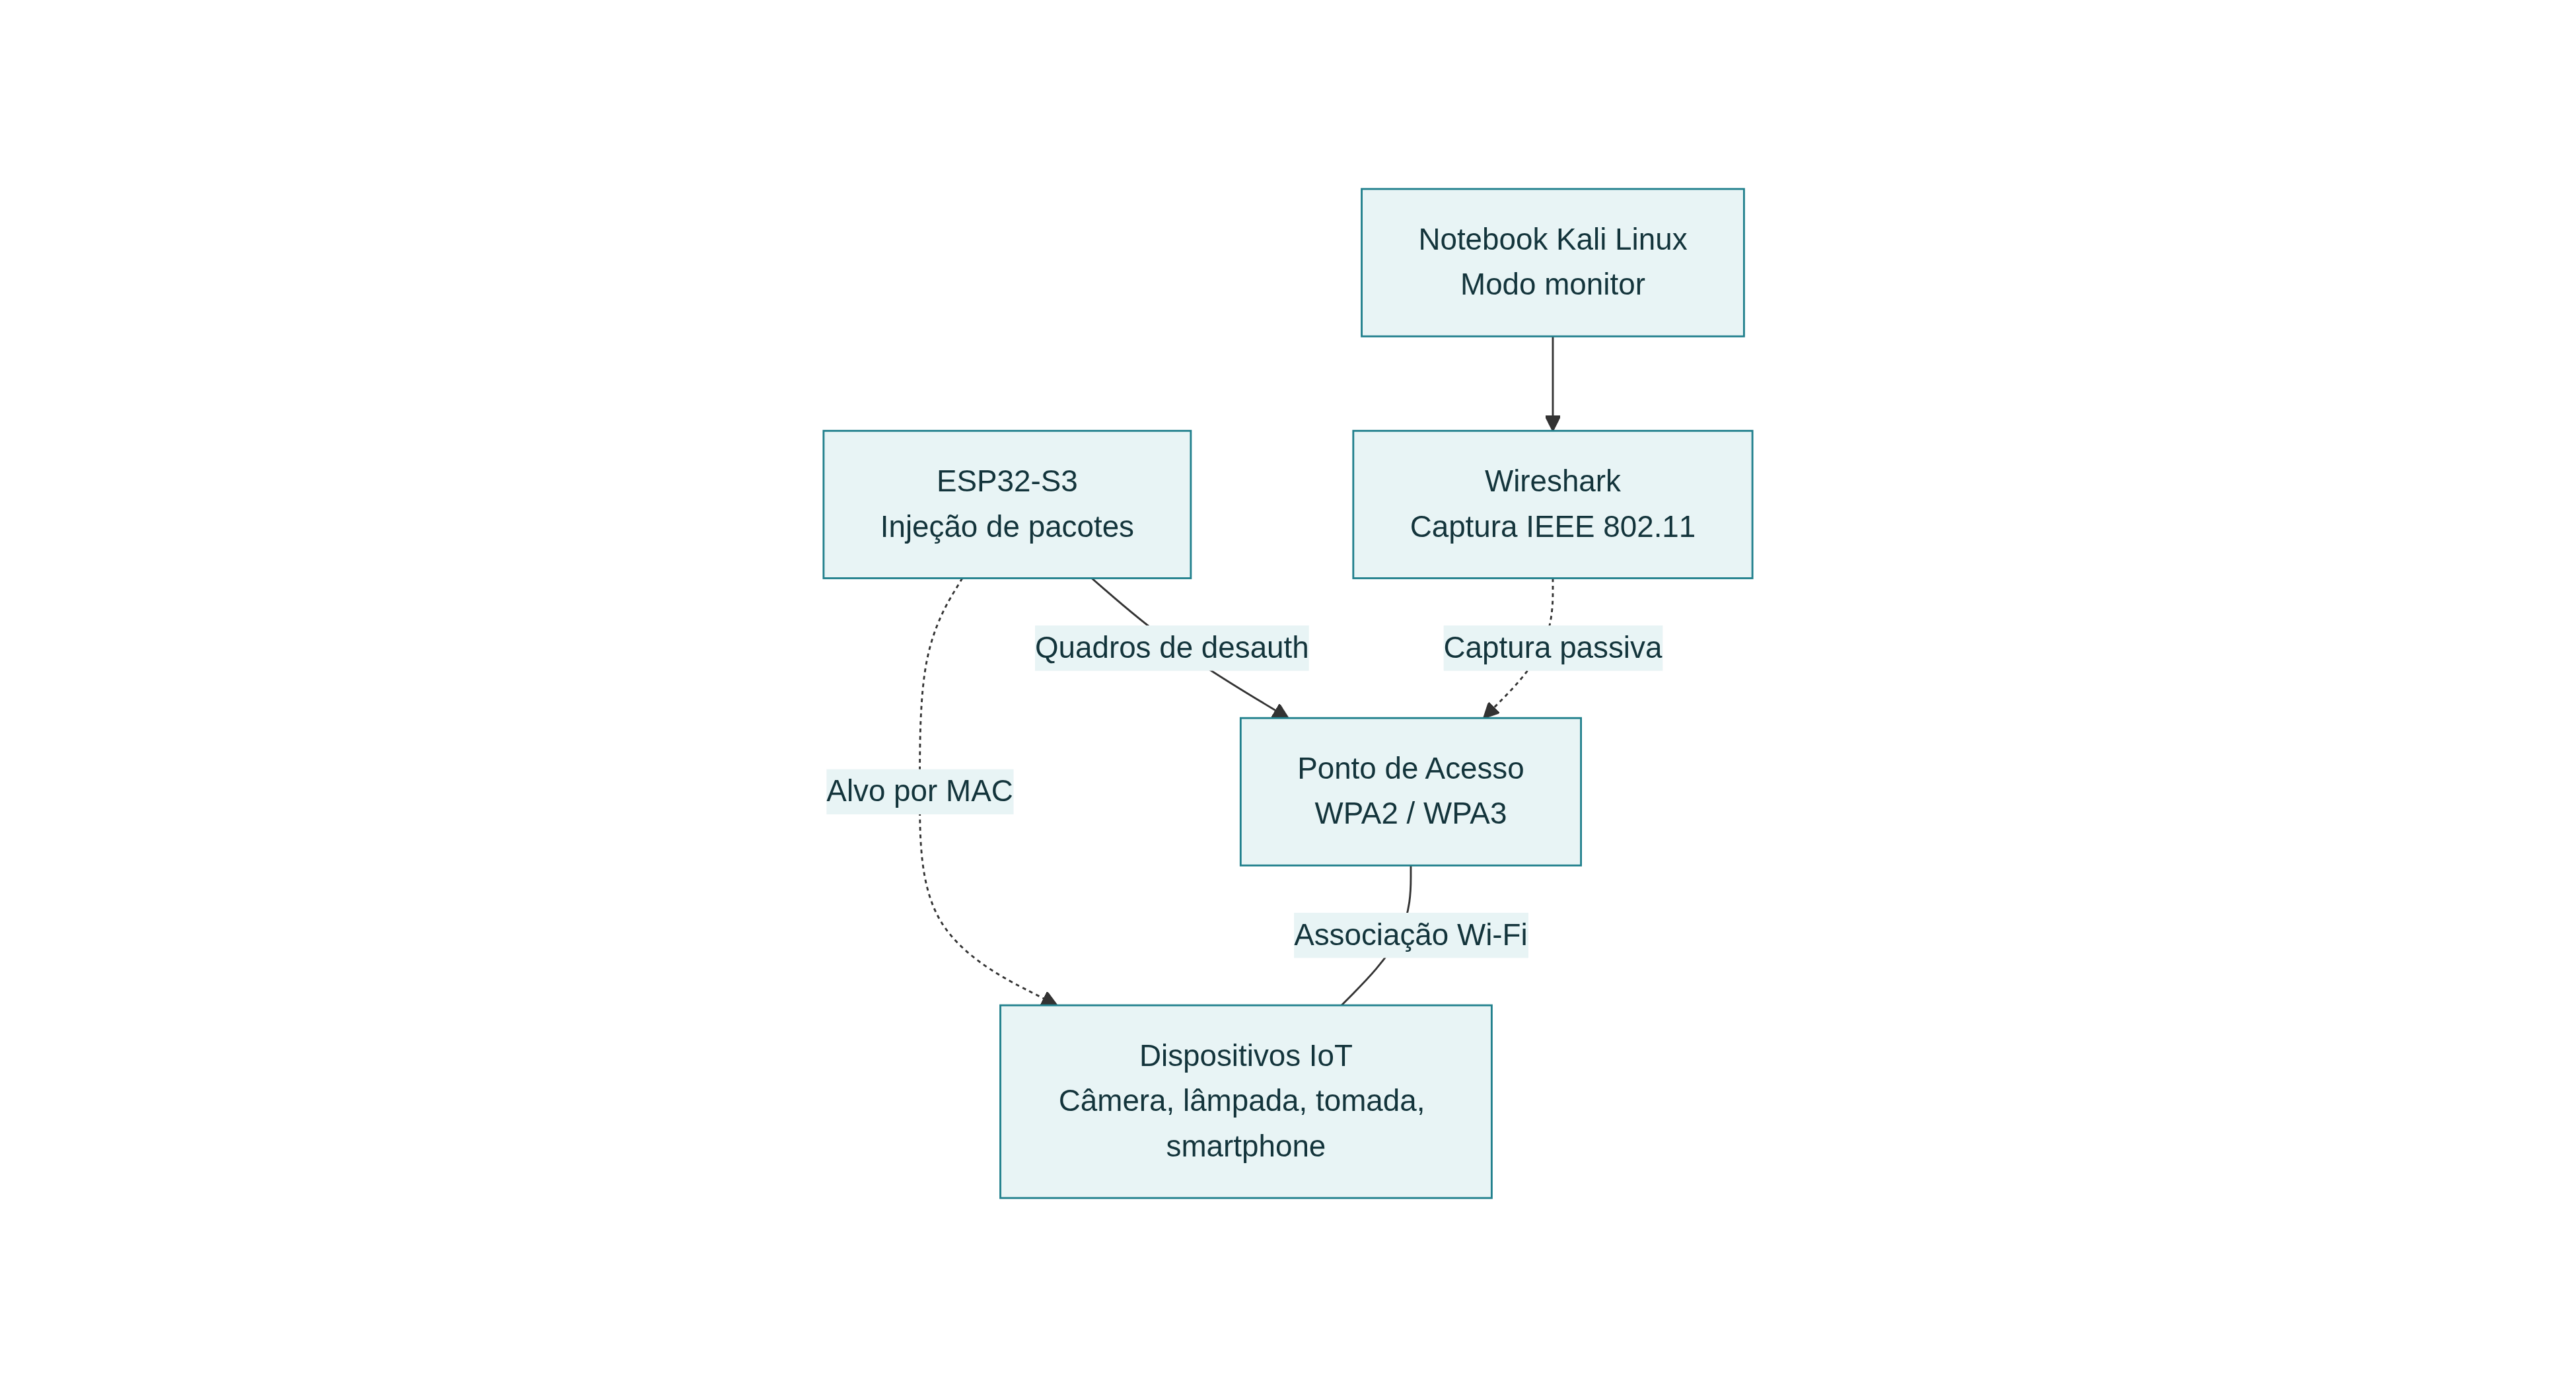
\includegraphics[
        width=0.88\textwidth,
        height=0.60\textheight,
        keepaspectratio
    ]{diagrama_blocos.jpg}
    \legend{Fonte: elaborado pelo autor (2026).}
\end{figure}

Como mostra a Figura~\ref{fig:diagrama_blocos}, a arquitetura teve quatro responsabilidades. O roteador e seu painel criaram a rede e definiram canal, segurança e PMF. O T-Embed CC1101 Plus, por meio do rádio Wi-Fi do ESP32-S3, transmitiu os quadros de desautenticação contra o dispositivo selecionado pelo endereço MAC. A câmera, a lâmpada e a tomada foram os dispositivos avaliados, e o \textit{smartphone} serviu como referência. Por fim, a estação de captura (Kali Linux, adaptador AR9271 em modo monitor) apenas registrou o tráfego e executou o \textit{ping}, sem participar da geração do ataque.

\section{Fluxograma do procedimento experimental}
\label{sec:atividades_experimento}

A Figura~\ref{fig:fluxograma_experimento} apresenta a sequência efetivamente seguida em cada ensaio, desde a configuração do ponto de acesso até a análise dos arquivos.

\begin{figure}[htbp]
\centering
\caption{Fluxograma do procedimento experimental}
\label{fig:fluxograma_experimento}
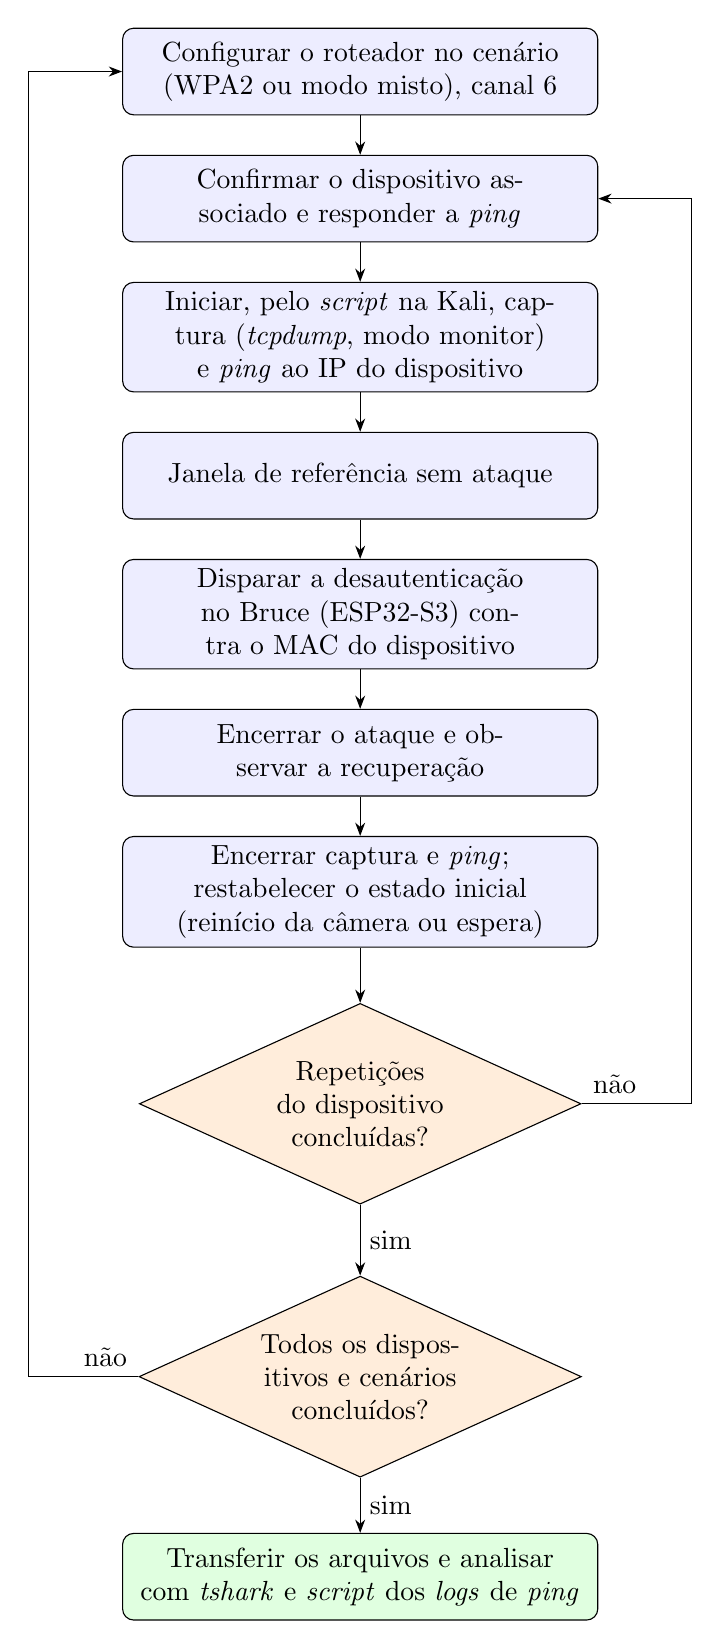
\begin{tikzpicture}[font=\normalsize, >=Stealth, node distance=5mm,
  b/.style={draw, rounded corners, fill=blue!7, text width=58mm, align=center, minimum height=11mm},
  d/.style={draw, diamond, aspect=2.2, fill=orange!14, text width=30mm, align=center, inner sep=1pt}]
\node[b] (s1) {Configurar o roteador no cenário (WPA2 ou modo misto), canal 6};
\node[b, below=of s1] (s2) {Confirmar o dispositivo associado e responder a \textit{ping}};
\node[b, below=of s2] (s3) {Iniciar, pelo \textit{script} na Kali, captura (\textit{tcpdump}, modo monitor) e \textit{ping} ao IP do dispositivo};
\node[b, below=of s3] (s4) {Janela de referência sem ataque};
\node[b, below=of s4] (s5) {Disparar a desautenticação no Bruce (ESP32-S3) contra o MAC do dispositivo};
\node[b, below=of s5] (s6) {Encerrar o ataque e observar a recuperação};
\node[b, below=of s6] (s7) {Encerrar captura e \textit{ping}; restabelecer o estado inicial (reinício da câmera ou espera)};
\node[d, below=7mm of s7] (q1) {Repetições do dispositivo concluídas?};
\node[d, below=9mm of q1] (q2) {Todos os dispositivos e cenários concluídos?};
\node[b, below=7mm of q2, fill=green!12] (s8) {Transferir os arquivos e analisar com \textit{tshark} e \textit{script} dos \textit{logs} de \textit{ping}};
\foreach \a/\b in {s1/s2,s2/s3,s3/s4,s4/s5,s5/s6,s6/s7,s7/q1} \draw[->] (\a) -- (\b);
\draw[->] (q1) -- node[right] {sim} (q2);
\draw[->] (q2) -- node[right] {sim} (s8);
\draw[->] (q1.east) -- node[above, pos=0.3] {não} ++(14mm,0) |- (s2.east);
\draw[->] (q2.west) -- node[above, pos=0.3] {não} ++(-14mm,0) |- (s1.west);
\end{tikzpicture}
\legend{Fonte: elaborado pelo autor (2026). No ensaio piloto, a captura foi feita pelo Wireshark, sem \textit{ping}.}
\end{figure}

Na Figura~\ref{fig:fluxograma_experimento}, a captura e o \textit{ping} foram iniciados juntos, antes do ataque, para registrar uma janela de referência; o ataque foi disparado manualmente no menu Wi-Fi do Bruce; e, ao final, o estado inicial do dispositivo foi restabelecido antes da repetição seguinte. Na câmera, esse restabelecimento exigiu reinício manual, porque ela não se reassociou sozinha. O protocolo completo, passo a passo, é detalhado no Apêndice~\ref{sec:protocolo}.

\section{Cadeia de processamento dos dados}
\label{sec:dados_captura}

Cada ensaio gerou um par de arquivos com o mesmo identificador, no formato \texttt{DISPOSITIVO\_CENÁRIO\_Rnn} (por exemplo, \texttt{LAMP\_WPA2\_R01.pcapng} e \texttt{LAMP\_WPA2\_R01\_ping.txt}). Ambos foram produzidos na máquina virtual Kali por um \textit{script} auxiliar, que, a partir do nome do ensaio, do IP do dispositivo e do canal, iniciava em paralelo o \textit{tcpdump} na interface em modo monitor e o \textit{ping} ao dispositivo, e os encerrava ao final. Os arquivos foram então transferidos para o computador hospedeiro, onde foi feita toda a análise. A Figura~\ref{fig:estrutura_evidencias} resume essa cadeia.

\begin{figure}[htb]
\centering
\caption{Cadeia de processamento das evidências de cada ensaio}
\label{fig:estrutura_evidencias}
\resizebox{\textwidth}{!}{%
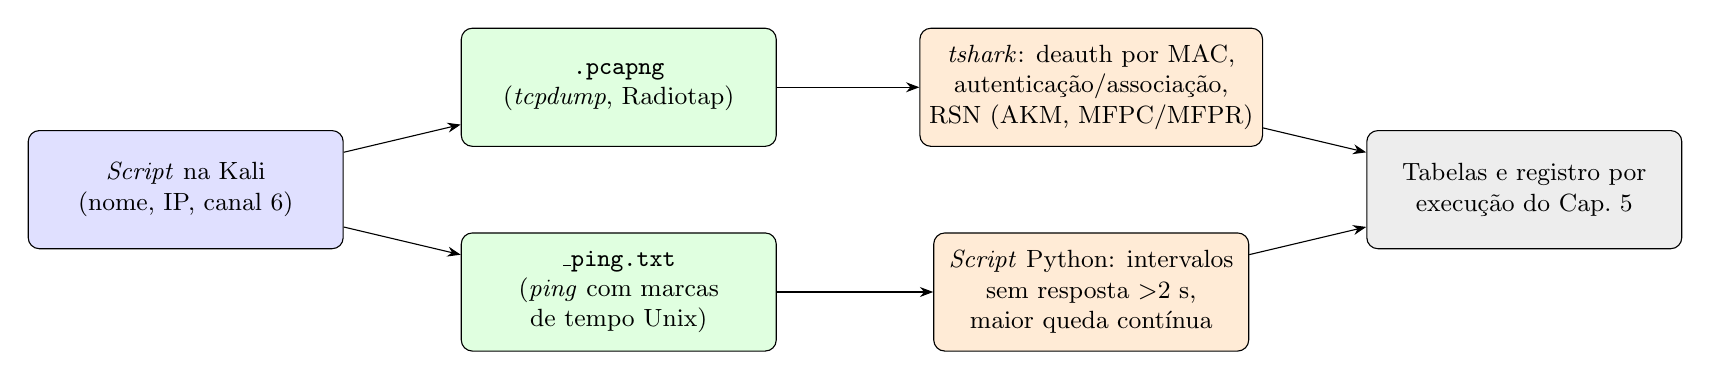
\begin{tikzpicture}[font=\small, >=Stealth,
  e/.style={draw, rounded corners, minimum width=40mm, minimum height=15mm, align=center}]
\node[e, fill=blue!12] (exec) at (0,0) {\textit{Script} na Kali\\(nome, IP, canal 6)};
\node[e, fill=green!12] (pcap) at (5.5,1.3) {\texttt{.pcapng}\\(\textit{tcpdump}, Radiotap)};
\node[e, fill=green!12] (ping) at (5.5,-1.3) {\texttt{\_ping.txt}\\(\textit{ping} com marcas\\de tempo Unix)};
\node[e, fill=orange!16] (ts) at (11.5,1.3) {\textit{tshark}: deauth por MAC,\\autenticação/associação,\\RSN (AKM, MFPC/MFPR)};
\node[e, fill=orange!16] (py) at (11.5,-1.3) {\textit{Script} Python: intervalos\\sem resposta $>$2~s,\\maior queda contínua};
\node[e, fill=gray!14] (tab) at (17,0) {Tabelas e registro por\\execução do Cap.~5};
\draw[->] (exec) -- (pcap); \draw[->] (exec) -- (ping);
\draw[->] (pcap) -- (ts); \draw[->] (ping) -- (py);
\draw[->] (ts) -- (tab); \draw[->] (py) -- (tab);
\end{tikzpicture}}
\legend{Fonte: elaborado pelo autor (2026).}
\end{figure}

Como indica a Figura~\ref{fig:estrutura_evidencias}, as duas vertentes foram processadas separadamente:

\begin{itemize}
    \item \textbf{Das capturas (\textit{tshark})} vieram: o número de quadros de desautenticação com o endereço do dispositivo como origem ou destino (filtro de subtipo 12); os quadros de autenticação e associação, usados para identificar perda de associação; e os campos do elemento RSN (AKM, MFPC e MFPR) dos \textit{beacons} e dos \textit{Association Requests}.
    \item \textbf{Dos \textit{logs} de \textit{ping}} vieram: o tempo acumulado sem resposta (soma dos intervalos entre respostas consecutivas superiores a 2~s), a fração desse tempo sobre a duração do \textit{log} e a maior queda contínua.
\end{itemize}

A sincronização entre as duas fontes decorre de ambas terem sido geradas pela mesma máquina, com o mesmo relógio: o \textit{ping} foi executado com marcas de tempo absolutas (época Unix) em cada resposta, e o arquivo de captura registra o instante absoluto de cada quadro. Nos arquivos verificados (\texttt{LAMP\_WPA2\_R01}, \texttt{TOMADA\_WPA2\_R01} e \texttt{CAM\_WPA3\_R01}), a primeira resposta de \textit{ping} ocorreu até 0,5~s após o primeiro quadro capturado, o que confirma o início conjunto. Não houve sincronização com relógio externo, de modo que a comparação é válida entre as duas fontes de um mesmo ensaio, e não com horários de outros equipamentos. Os \textit{logs} contêm respostas marcadas como duplicadas (\texttt{DUP!}), acompanhadas do aviso \textit{wrong data byte} e de tempo \texttt{0.000~ms}; essas respostas, inclusive a primeira de cada série, que o \textit{ping} não marca como duplicada, foram descartadas no cálculo, feito pelo \textit{script} \texttt{src/analisa\_ping.py}, por corresponderem a eco de conteúdo corrompido e não a uma resposta válida, conforme a definição da métrica de perda de pacotes na Seção~\ref{subsec:dicionario_metricas}.

\section{Registro fotográfico do ambiente montado}
\label{sec:registro_fotografico}

Esta seção apresenta o registro fotográfico dos principais equipamentos montados na bancada experimental: o ponto de acesso, a plataforma de ataque e dois dos dispositivos IoT avaliados (câmera IP e tomada inteligente).

A Figura~\ref{fig:foto_roteador} apresenta o roteador TP-Link EX1500 empregado
como ponto de acesso da rede de teste, responsável por disponibilizar a rede
Wi-Fi e pelas configurações de segurança WPA2 e modo misto.

\begin{figure}[htb]
    \centering
    \caption{Roteador TP-Link EX1500 utilizado como ponto de acesso}
    \label{fig:foto_roteador}
    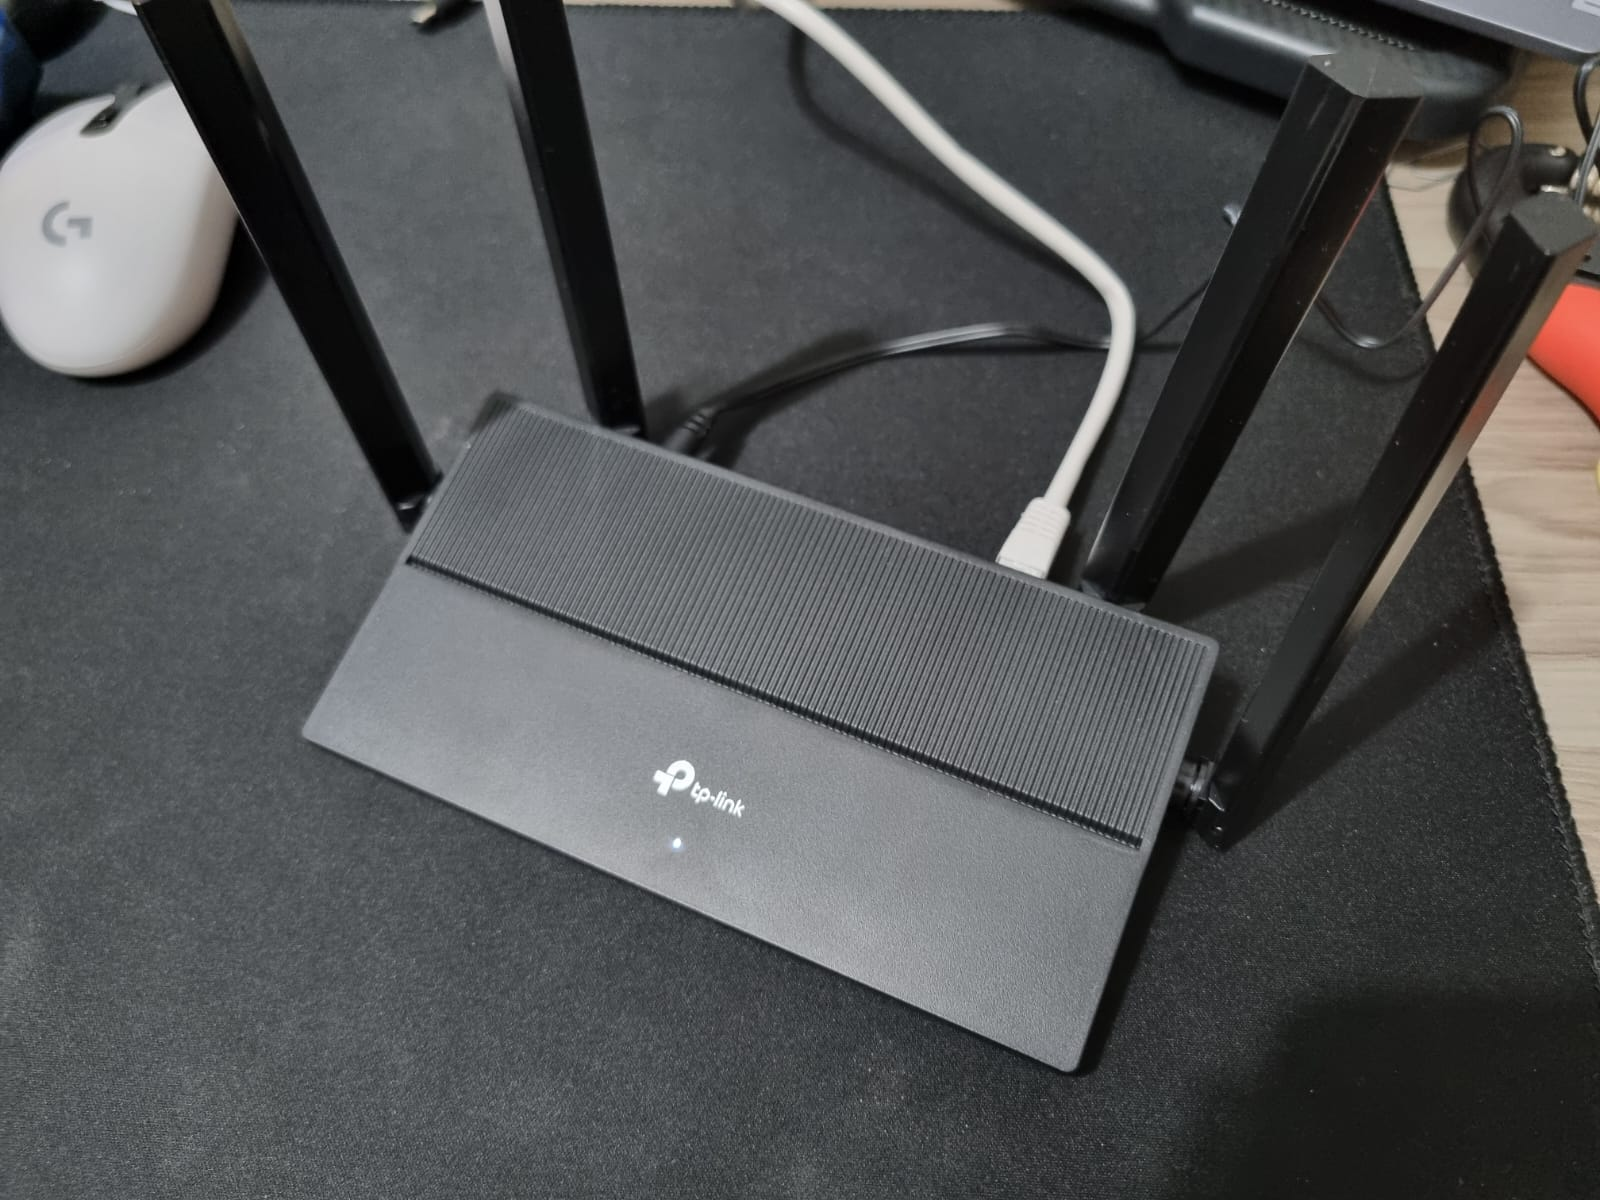
\includegraphics[width=0.72\textwidth,height=0.42\textheight,keepaspectratio]{foto_roteador.jpg}
    \legend{Fonte: elaborado pelo autor (2026).}
\end{figure}

A Figura~\ref{fig:foto_lilygo} apresenta a plataforma LILYGO T-Embed CC1101 Plus,
baseada em ESP32-S3 e executando o \textit{firmware} Bruce~1.16.1, utilizada como
plataforma de ataque. A tela exibe o menu de funções Wi-Fi do \textit{firmware}.

\begin{figure}[htb]
    \centering
    \caption{Plataforma LILYGO T-Embed CC1101 Plus com \textit{firmware} Bruce}
    \label{fig:foto_lilygo}
    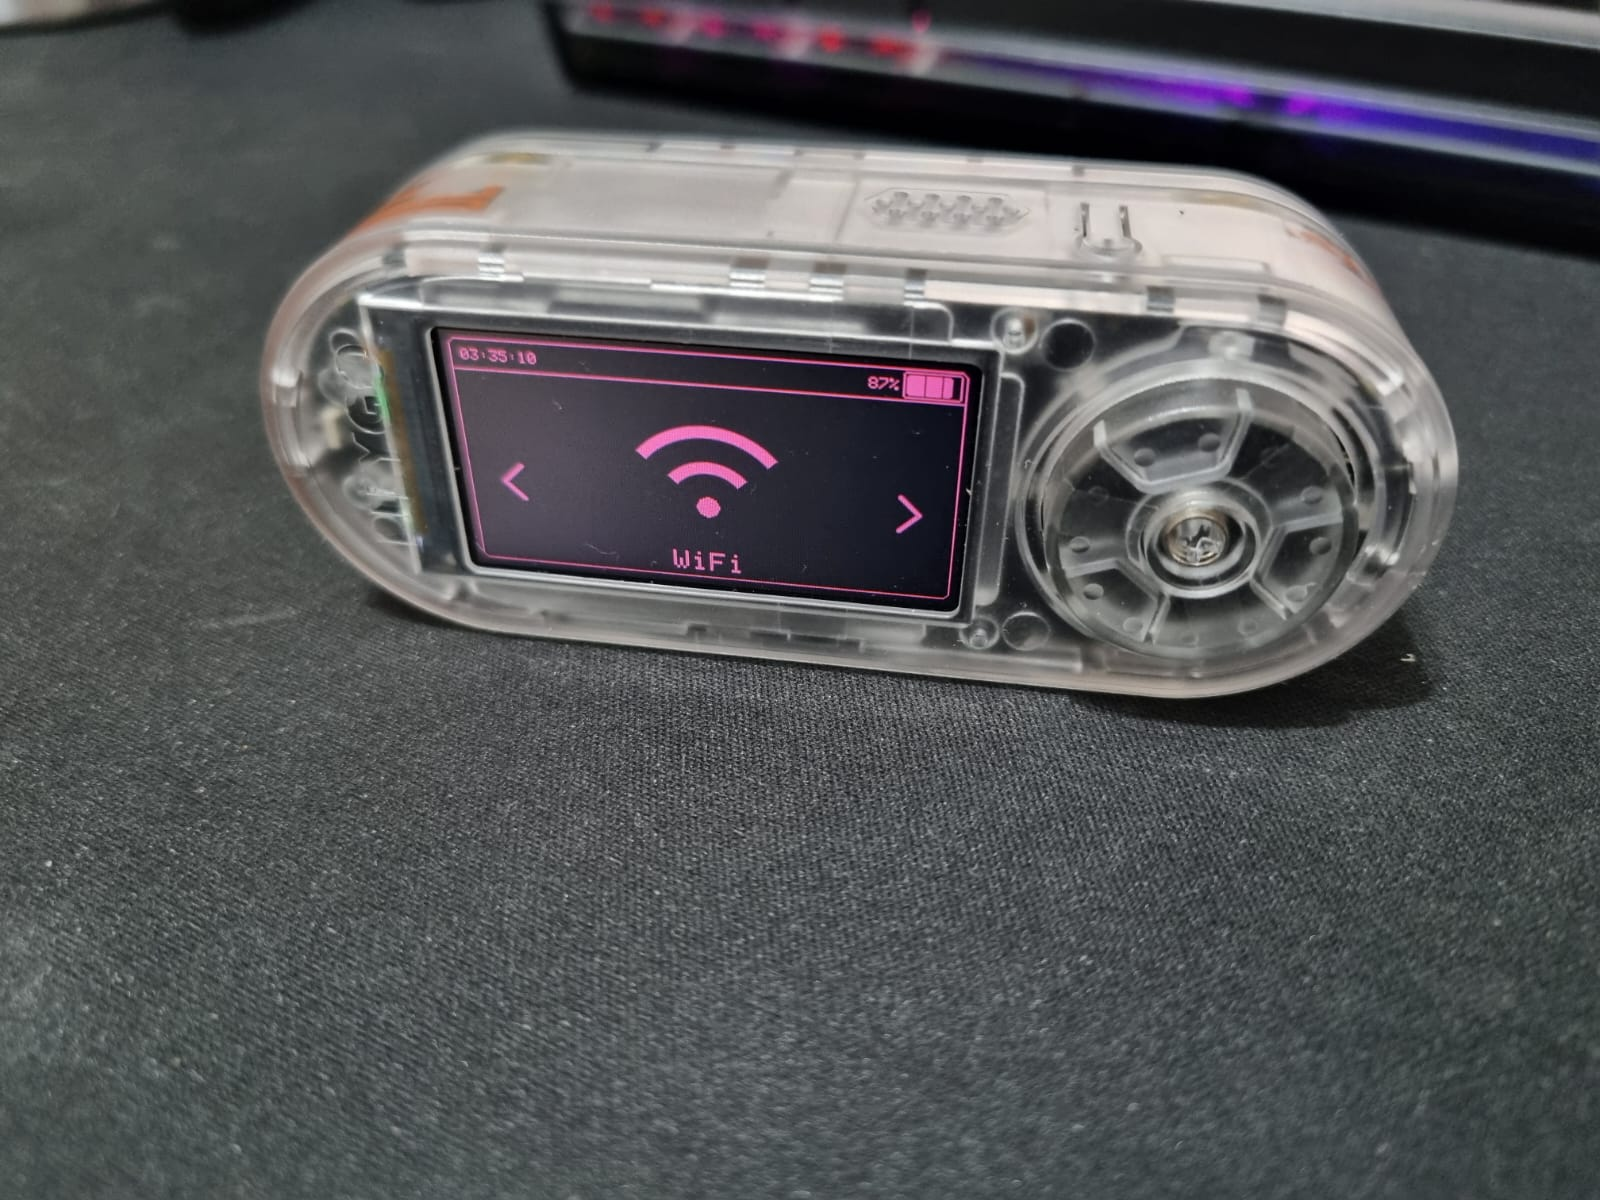
\includegraphics[width=0.72\textwidth,height=0.42\textheight,keepaspectratio]{foto_lilygo.jpg}
    \legend{Fonte: elaborado pelo autor (2026).}
\end{figure}

A Figura~\ref{fig:foto_camera} apresenta a câmera IP Xiaomi (identificada
comercialmente como Mi 360 PTZ 2K), utilizada tanto no ensaio piloto quanto nos
ensaios do conjunto completo de dispositivos.

\begin{figure}[htb]
    \centering
    \caption{Câmera IP Xiaomi utilizada como dispositivo IoT avaliado}
    \label{fig:foto_camera}
    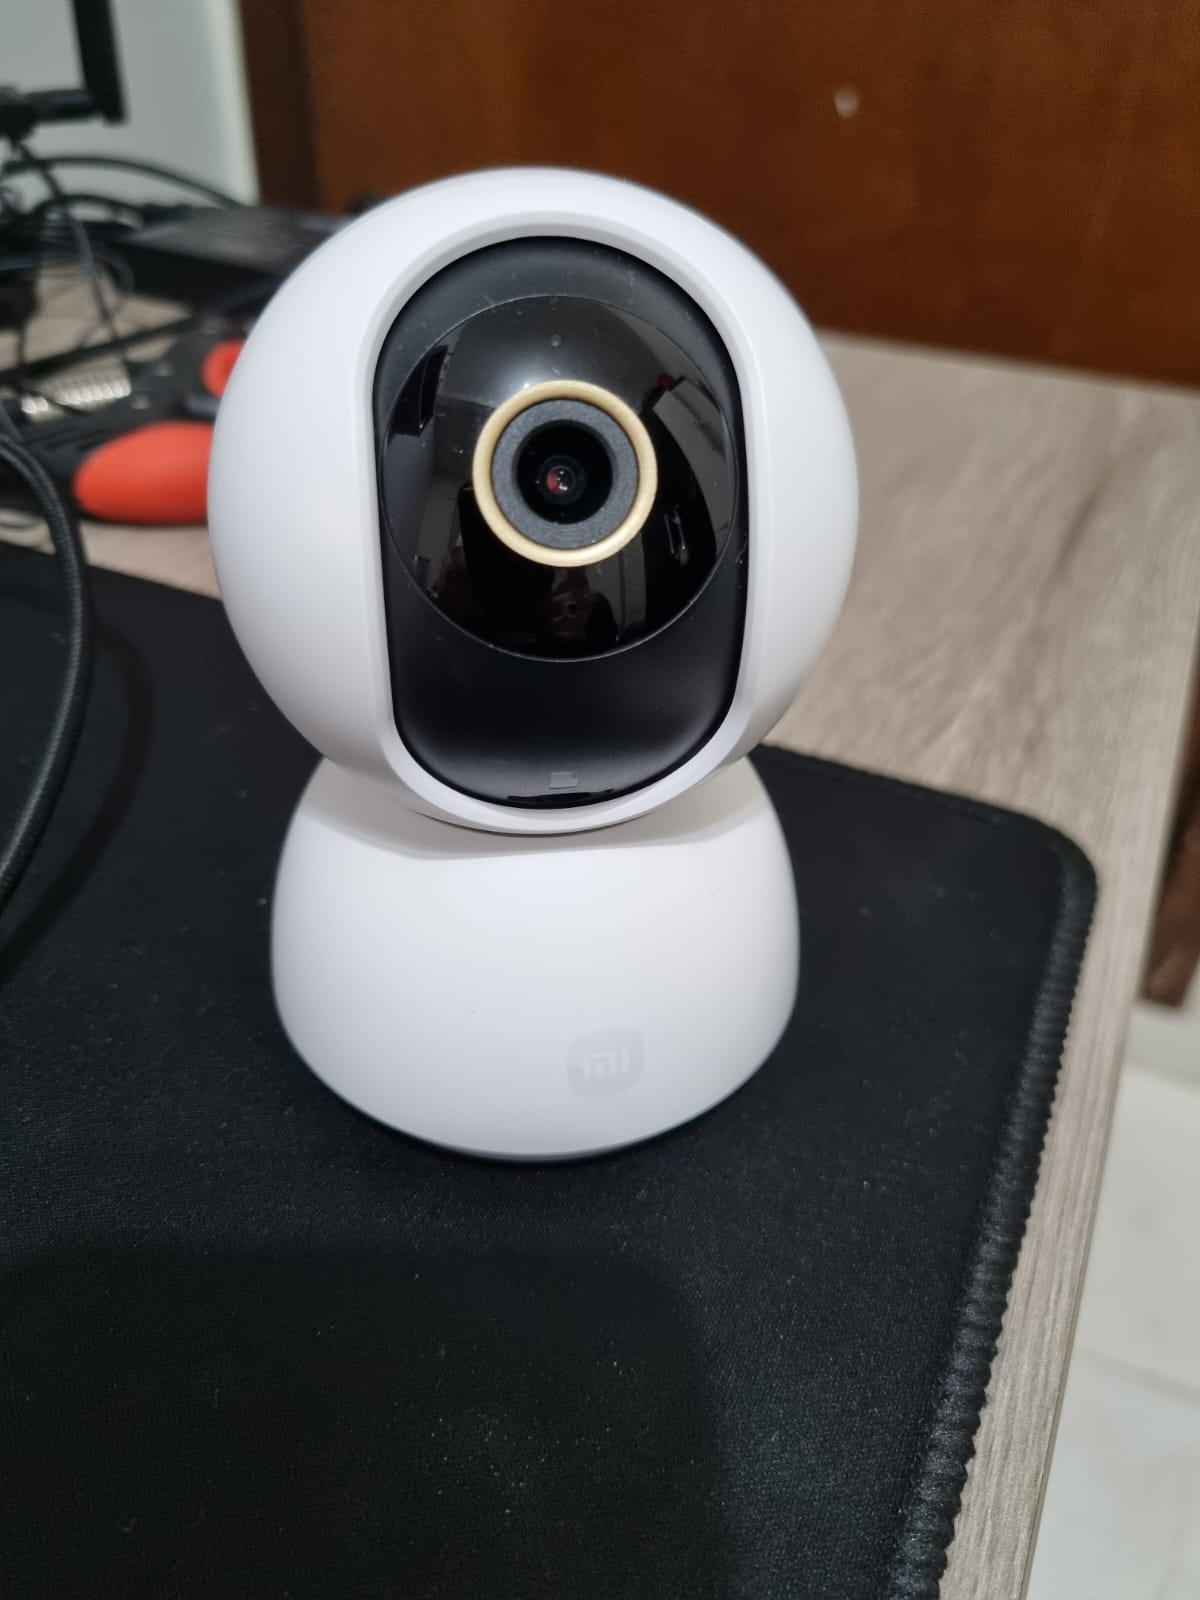
\includegraphics[width=0.60\textwidth,height=0.42\textheight,keepaspectratio]{foto_camera.jpg}
    \legend{Fonte: elaborado pelo autor (2026).}
\end{figure}

A Figura~\ref{fig:foto_tomada} apresenta a tomada inteligente, um dos
dispositivos IoT avaliados no experimento, conectada à rede de teste.

\begin{figure}[htb]
    \centering
    \caption{Tomada inteligente utilizada como dispositivo IoT avaliado}
    \label{fig:foto_tomada}
    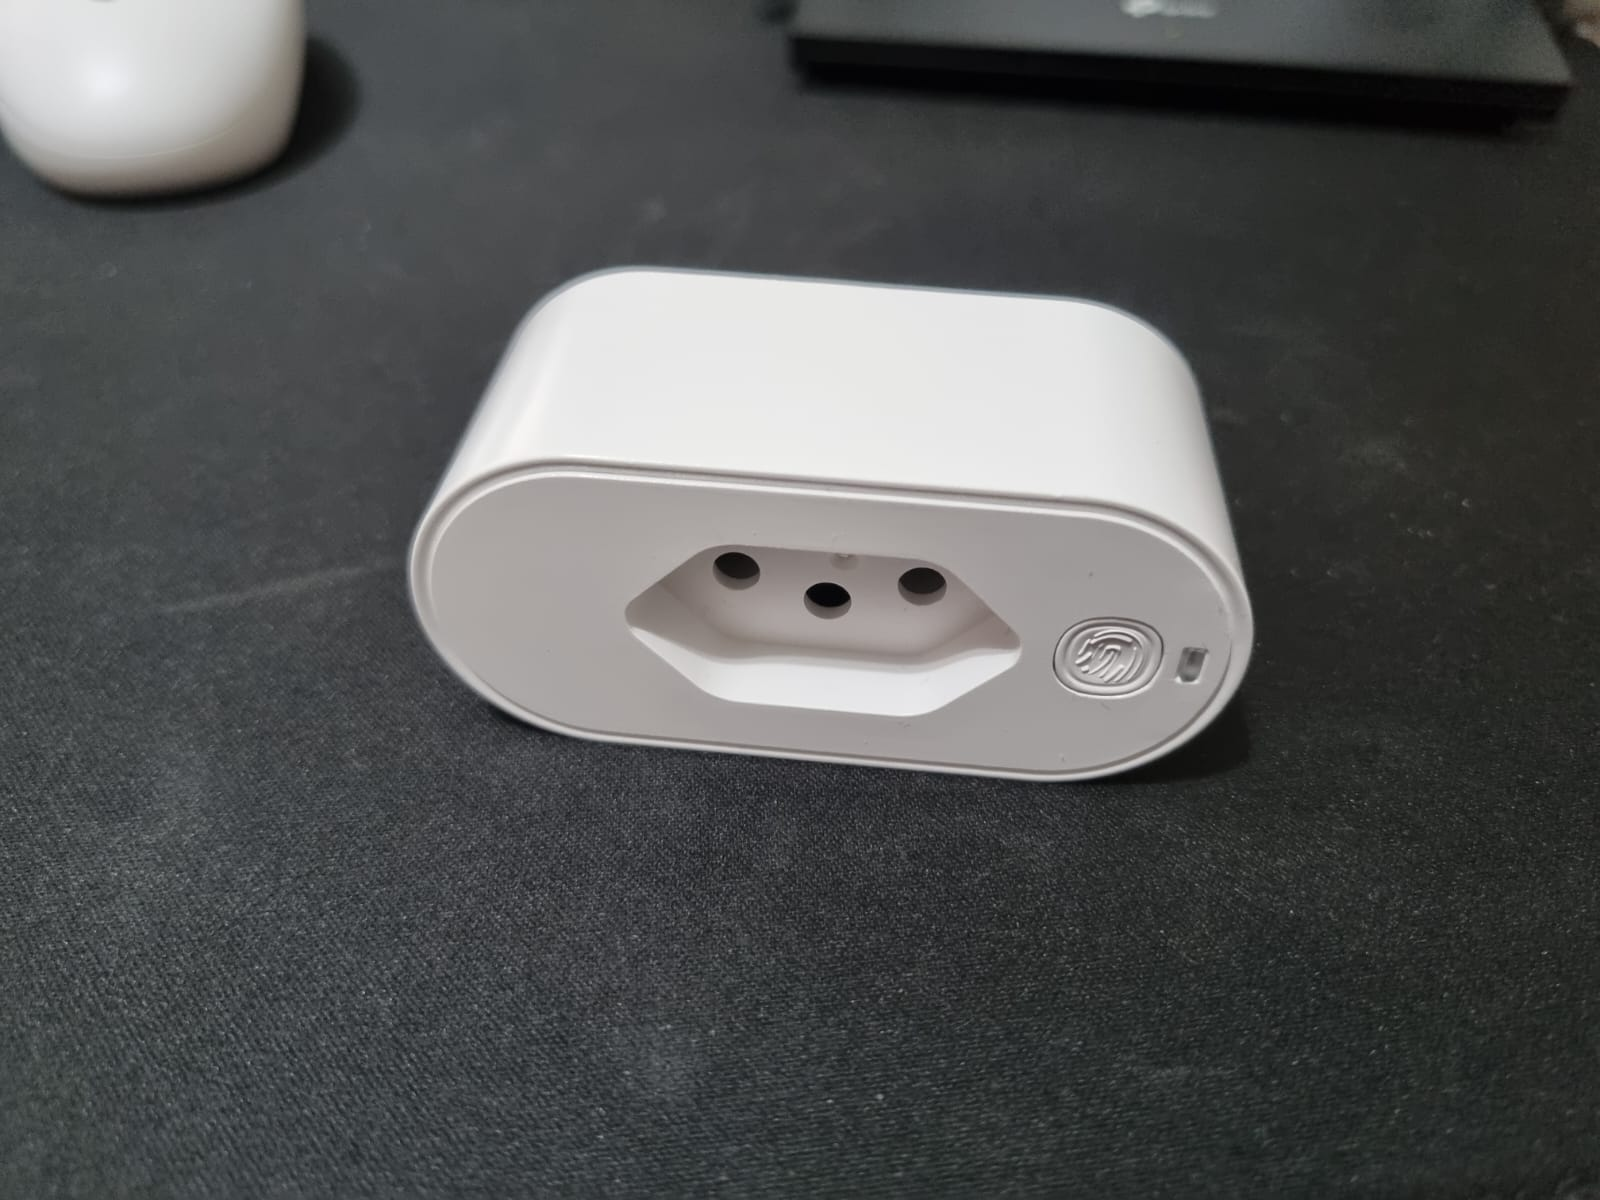
\includegraphics[width=0.72\textwidth,height=0.42\textheight,keepaspectratio]{foto_tomada.jpg}
    \legend{Fonte: elaborado pelo autor (2026).}
\end{figure}

\section{Critérios de validação aplicados}
\label{sec:criterios_validacao}

O ambiente foi considerado validado com base em evidências técnicas. Cada configuração de segurança foi validada pelo painel do roteador e pelos \textit{beacons} capturados, que registraram AKM e bits de PMF coerentes com a configuração pretendida. A associação de cada dispositivo foi validada pela resposta a \textit{ping} no início do ensaio. A captura foi considerada válida quando o adaptador gravou quadros IEEE~802.11 do canal 6 em arquivo \texttt{.pcapng} legível, o que ocorreu em todos os ensaios. A execução do ataque foi validada pela presença, na captura, de quadros de desautenticação com o endereço do dispositivo como origem ou destino; a execução \texttt{PHONE\_WPA3\_R02}, sem quadros de desautenticação direcionados ao \textit{smartphone}, não atendeu a esse critério. Além disso, uma execução foi considerada válida quando houve linha de base, isto é, respostas normais ao \textit{ping} antes do primeiro quadro de desautenticação direcionado ao dispositivo; nas execuções válidas, essa linha de base variou de cerca de 8,5~s a 105~s (Tabela~\ref{tab:registro-execucoes}). As execuções \texttt{CAM\_WPA2\_R05} e \texttt{CAM\_WPA2\_R06} não atenderam a esse critério e foram invalidadas: os quadros de desautenticação direcionados à câmera começaram aos 2,6~s e aos 0,5~s da captura, respectivamente, sem linha de base com \textit{ping} normal.

\section{Limitações do ambiente}
\label{sec:limitacoes_ambiente}

Os resultados ficam delimitados aos equipamentos, versões, configurações e cenários efetivamente utilizados; a amostra foi não probabilística e intencional, e os resultados não devem ser generalizados para todos os roteadores, dispositivos IoT ou redes IEEE~802.11.

No ambiente executado, as principais limitações foram: o número de repetições inferior ao planejado para a câmera e para o modo misto; a ausência de condições de WPA2 com PMF e de WPA3 exclusivo; a operação restrita a 2,4~GHz da plataforma de ataque e do adaptador de captura; o agrupamento dos ensaios por cenário, que faz o horário variar junto com a configuração; a distância entre os equipamentos, que não foi medida, e a potência de transmissão e a carga da rede, registradas mas não controladas como variáveis do ensaio (Quadro~\ref{quad:condicoes}); e a sincronização das fontes apenas pelo relógio da máquina virtual. Interferências de radiofrequência de redes vizinhas e atualizações automáticas dos dispositivos não foram controladas.

% !TeX root = ../main.tex
% !TeX encoding = UTF-8

\chapter{Análise de Resultados}

\label{cap:analise_resultados}

\section{Delimitação dos resultados apresentados}

Este capítulo apresenta os resultados da montagem e da execução do ambiente experimental destinado à análise de vulnerabilidades em redes IEEE 802.11 com dispositivos IoT. A apresentação inicia-se pela validação da estação de captura, pela observação funcional de referência de uma câmera IP e por um ensaio piloto de desautenticação contra essa câmera, e segue para o conjunto completo de dispositivos --- câmera IP, lâmpada inteligente, tomada inteligente e \textit{smartphone} de referência ---, nos cenários WPA2 e modo misto WPA2/WPA3. As evidências utilizadas são as saídas de comandos, as capturas de tela, os arquivos de captura de tráfego no formato PCAPNG e os \textit{logs} de \textit{ping} sincronizados, todos analisados com o Wireshark e com a ferramenta de linha de comando \textit{tshark}.



O escopo executado contempla a maior parte do planejamento descrito na metodologia: no cenário WPA2 foram realizadas três repetições independentes por dispositivo para a tomada, a lâmpada e o \textit{smartphone}, com medição dos tempos de indisponibilidade por \textit{ping}; e o cenário com WPA3 habilitado foi incluído na forma de modo misto (WPA2/WPA3). A câmera é um caso à parte: no cenário WPA2, teve duas execuções válidas com \textit{ping} (\texttt{CAM\_WPA2\_R03} e \texttt{CAM\_WPA2\_R04}), além do ensaio piloto, sem \textit{ping}; o arquivo \texttt{CAM\_WPA2\_R02}, apesar do nome, foi gravado com o ponto de acesso em modo misto e é tratado como ensaio desse cenário. Mantêm-se como delimitações esse número reduzido de repetições da câmera (cujo equipamento exige reinício manual a cada teste), o número reduzido de repetições no cenário misto (uma execução para a tomada e para a lâmpada, duas para a câmera e para o \textit{smartphone}) e a impossibilidade de testar os dispositivos IoT em WPA3 puro, uma vez que câmera e tomada não suportam esse protocolo.



Todos os indicadores quantitativos apresentados neste capítulo são derivados diretamente dos arquivos de captura e dos \textit{logs} de \textit{ping}, e não de transcrição manual de imagens: as contagens de quadros, o número de quadros de desautenticação, a duração das capturas, as janelas e taxas de emissão do ataque e a segurança efetivamente negociada por cada dispositivo foram extraídos dos arquivos de captura com o \textit{tshark}, enquanto os tempos sem resposta e as demais métricas de conectividade foram calculados a partir dos \textit{logs} de \textit{ping}. Quanto às ferramentas, a captura do ensaio piloto foi feita com o Wireshark (motor \textit{dumpcap}) e a dos ensaios do conjunto completo com o \textit{tcpdump}, ambos operando o adaptador em modo monitor na Kali Linux; a análise de todas as capturas foi feita com o Wireshark e o \textit{tshark}. O ensaio piloto da câmera, descrito nas seções iniciais, é mantido por documentar a integração inicial do ambiente; os resultados do conjunto completo de dispositivos e a comparação entre os cenários com e sem PMF são apresentados na Seção~\ref{subsec:consolidacao_tabelas}.



\section{Procedimentos de teste}

Esta seção descreve como o ambiente foi efetivamente exercitado e quais instrumentos foram empregados. Por se tratar de um estudo de segurança de redes, e não de um sistema de informação com interface própria, os procedimentos de teste correspondem à verificação funcional da instrumentação, à integração dos componentes do ambiente e a um ensaio direcionado de desautenticação, e não a baterias de testes de software convencionais.

\subsection{Tipos de testes aplicados}

Nesta etapa foram aplicados três tipos de verificação. O primeiro corresponde a um \textbf{teste de validação da estação de captura}, destinado a confirmar que o adaptador em modo monitor registrava quadros IEEE~802.11 no canal da rede de teste. O segundo é um \textbf{teste funcional de referência}, no qual a câmera foi observada em operação normal, sem intervenção da plataforma de baixo custo. O terceiro é um \textbf{ensaio direcionado} ao endereço da câmera, durante o qual foram inspecionados os quadros classificados como \textit{Deauthentication}.

O procedimento foi organizado em uma condição de referência, sem intervenção do LILYGO, e em um ensaio direcionado ao endereço da câmera selecionada. Na referência, o pesquisador relatou funcionamento normal da imagem ao vivo, enquanto a captura apresentou quadros IEEE 802.11 associados ao ponto de acesso e à câmera. No ensaio, foram identificados registros classificados como \textit{Deauthentication}. As durações do ensaio piloto relatadas nesta seção derivam dos tempos relativos da própria captura; os tempos de indisponibilidade por \textit{ping} só foram medidos no conjunto completo de dispositivos (Seção~\ref{subsec:consolidacao_tabelas}).

No ensaio piloto descrito nesta seção não foram aplicados testes sistemáticos de desempenho (tempo de resposta e carga), as três execuções independentes por cenário nem a comparação entre as configurações WPA2 e WPA3. Esses procedimentos foram realizados posteriormente, para o conjunto completo de dispositivos, e são apresentados na Seção~\ref{subsec:consolidacao_tabelas}.

\subsection{Ferramentas e dispositivos utilizados}

A bancada efetivamente utilizada neste ensaio corresponde à descrita na metodologia: o roteador TP-Link EX1500 como ponto de acesso; o LILYGO T-Embed CC1101 Plus (\textit{firmware} Bruce 1.16.1) como plataforma de teste; uma câmera Xiaomi identificada comercialmente como Mi 360 PTZ 2K; um \textit{notebook} com Kali Linux executado em máquina virtual VirtualBox; um adaptador USB Qualcomm Atheros AR9271; e o Wireshark 4.6.6. O ambiente observado utilizou a rede TCC\_LAB em 2,4 GHz, canal 6, com largura de 20 MHz. O protocolo de segurança foi documentado no painel administrativo do roteador, apresentado na Figura~\ref{fig:painel_roteador_wpa2}, que registra a rede TCC\_LAB configurada com segurança WPA2-PSK[AES], isto é, WPA2 com criptografia AES/CCMP. A opção de \textit{Protected Management Frames} (PMF) não aparece habilitada para esse modo nesse \textit{firmware}. Ressalta-se que o painel registra apenas a configuração do ponto de acesso, e não a segurança efetivamente negociada por cada estação; esta é verificada no elemento RSN dos quadros de associação, cujas evidências constam do Apêndice~\ref{sec:evidencias-rsn}. Nas capturas deste cenário, os \textit{beacons} do ponto de acesso anunciam somente o AKM~2 (PSK) e o bit MFPC~=~0, o que confirma, do lado do ponto de acesso, que o PMF não era oferecido; esse estado é coerente com o fato de o ataque de desautenticação ter sido efetivo, uma vez que o PMF, quando ativo, protege justamente os quadros de gerenciamento contra falsificação. Como este ensaio contempla apenas o cenário WPA2, ele não é classificado aqui como comparação entre configurações de segurança, comparação apresentada na Seção~\ref{subsec:consolidacao_tabelas}.

\begin{figure}[htb]
\centering
\caption{Configuração de segurança da rede de teste no painel do roteador}
\label{fig:painel_roteador_wpa2}
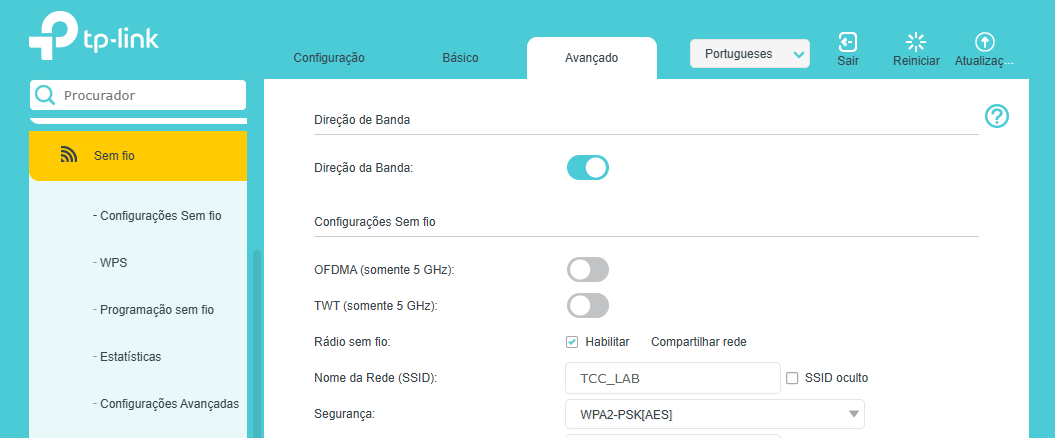
\includegraphics[width=0.9\textwidth]{painel_roteador_wpa2.png}
\legend{Fonte: captura do pesquisador no painel administrativo do TP-Link EX1500 (2026).}
\end{figure}



O Quadro~\ref{quad:config-documentada} reúne os componentes efetivamente utilizados na bancada do ensaio piloto, com seus modelos, versões de \textit{software}/\textit{firmware} e parâmetros de rádio, servindo de referência para a interpretação das evidências apresentadas nas seções seguintes.

\begin{quadro}[htbp]
\centering
\caption{Configuração efetivamente documentada}
\label{quad:config-documentada}
\small
\begin{tabular}{|>{\raggedright\arraybackslash}p{0.45\textwidth}|>{\raggedright\arraybackslash}p{0.45\textwidth}|}
\hline
\textbf{Componente} & \textbf{Registro} \\ \hline
Ponto de acesso & TP-Link EX1500; \textit{firmware} informado 1.13.0 \\ \hline
Plataforma de teste & LILYGO T-Embed CC1101 Plus; Bruce 1.16.1 \\ \hline
Câmera & Xiaomi, nome de rede chuangmi\_camera\_029a02; código de modelo PTZ 2K; \textit{firmware} 4.3.4\_0425 (Seção~\ref{sec:inventario}) \\ \hline
Estação de captura & Kali Linux em VirtualBox; Wireshark 4.6.6 \\ \hline
Adaptador & Qualcomm Atheros AR9271; USB 0cf3:9271; \textit{driver} ath9k\_htc \\ \hline
Condição de rádio & 2,4 GHz; canal 6; 2437 MHz; largura de 20 MHz \\ \hline
Segurança e PMF (configurados) & WPA2-PSK[AES] (AES/CCMP); PMF não habilitado no painel (Figura~\ref{fig:painel_roteador_wpa2}); \textit{beacon}: AKM~2, MFPC~=~0 (Apêndice~\ref{sec:evidencias-rsn}) \\ \hline
Acesso externo & Internet disponibilizada durante a preparação \\ \hline
\end{tabular}
\legend{Fonte: elaborado pelo autor a partir dos registros do ensaio (2026).}
\end{quadro}

\section{Métricas coletadas}

\subsection{Indicadores avaliados}

Os indicadores previstos para o estudo compreendem o funcionamento da câmera na condição de referência, a presença de quadros de desautenticação, o tempo de indisponibilidade funcional, o tempo de recuperação da associação, a ocorrência de recuperação automática, o total de quadros no ensaio, a comparação entre WPA2 e WPA3 e a realização de três repetições por cenário. A situação de cada indicador no ensaio piloto é consolidada ao final desta seção, distinguindo o que foi documentado do que não foi mensurado nesse ensaio; os valores medidos para todos os dispositivos são apresentados na Seção~\ref{subsec:consolidacao_tabelas}.

\subsection{Dicionário de métricas}
\label{subsec:dicionario_metricas}

Antes da apresentação dos resultados, esta subseção define cada métrica utilizada no capítulo e nas Tabelas~\ref{tab:registro-execucoes} e~\ref{tab:registro-metricas}. As definições separam grandezas que, embora relacionadas, não são equivalentes: segundos sem resposta, porcentagem de pacotes perdidos e porcentagem do tempo de observação medem coisas diferentes e não devem ser comparados entre si. Do mesmo modo, a perda de respostas a \textit{ping} não se confunde com a perda de associação, e a recuperação da rede não se confunde com a recuperação da função do dispositivo.

\begin{description}
    \item[Perda de pacotes ICMP (\%):] razão entre as requisições \textit{Echo Request} do \textit{Internet Control Message Protocol} (ICMP) sem resposta válida e o total de requisições enviadas ao dispositivo, multiplicada por 100. O \textit{ping} é executado a partir da estação de captura com o comando \texttt{ping -D -i 0.5}, isto é, com marcas de tempo absolutas e intervalo nominal de 0,5~s entre requisições; não foi definido tempo limite explícito por requisição, pois a opção \texttt{-W} não foi utilizada e, portanto, vigorou o comportamento padrão do \textit{iputils}. O total de requisições e as perdas são obtidos pela contagem dos números de sequência (\texttt{icmp\_seq}): uma sequência é considerada recebida quando há ao menos uma resposta válida com aquele número. As respostas duplicadas (\textit{DUP!}), que no \textit{log} vêm acompanhadas do aviso \textit{wrong data byte} e de tempo \texttt{0.000~ms}, são descartadas por corresponderem a eco de conteúdo corrompido, e não a uma nova resposta válida. A regra vale também para a primeira ocorrência desse eco, que o \textit{ping} não marca como duplicada, mas que traz o mesmo aviso e o mesmo tempo de \texttt{0.000~ms}. A porcentagem só tem sentido junto da janela sobre a qual foi calculada, que deve ser sempre informada.
    \item[Tempo acumulado sem resposta (s):] soma, dentro da janela observada, de todos os intervalos entre respostas válidas consecutivas que excedem o limiar de 2~s. Intervalos menores que o limiar são tratados como variação normal e não entram na soma. É a métrica apresentada como indisponibilidade nas tabelas deste capítulo.
    \item[Fração do tempo sem resposta (\%):] tempo acumulado sem resposta dividido pela duração do \textit{log} de \textit{ping} correspondente, multiplicado por 100. Não equivale à perda de pacotes ICMP nem à fração da janela de ataque, pois o \textit{log} de \textit{ping} pode começar antes e terminar depois do ataque.
    \item[Maior queda contínua (s):] o maior intervalo isolado entre duas respostas válidas consecutivas na janela observada. Distingue-se do tempo acumulado: um dispositivo com muitas quedas curtas pode ter tempo acumulado alto e maior queda contínua baixa, enquanto outro, com uma única queda longa, tem os dois valores iguais.
    \item[Recuperação de rede:] retorno das respostas válidas ao \textit{ping} de forma sustentada após a última queda. Pode ser \textit{automática}, quando ocorre sem intervenção, ou \textit{manual}, quando depende de ação do pesquisador.
    \item[Recuperação da função:] retorno do serviço que o usuário percebe, que é distinto da rede: a imagem ao vivo da câmera no aplicativo, a resposta da tomada a um comando de liga/desliga e a resposta da lâmpada a um comando no aplicativo. Um dispositivo pode voltar a responder a \textit{ping} sem que a função tenha sido restabelecida.
    \item[Perda de associação:] saída do dispositivo do estado associado ao ponto de acesso, confirmada por evidência de enlace, como a ausência de tráfego de dados do dispositivo seguida de quadros de autenticação/associação (reassociação), ou pela remoção do cliente na lista do roteador. \textbf{\textit{Ping} perdido não prova desassociação}, pois a ausência de resposta pode decorrer de congestionamento do canal, de perda de quadros ou de economia de energia do dispositivo.
    \item[Quadros de desautenticação:] número de quadros \textit{Deauthentication} (subtipo 0x0C) na captura, contados com filtro explícito e sempre acompanhados do recorte usado: (i) direcionados ao dispositivo, isto é, com o endereço do dispositivo como origem ou destino; (ii) em difusão (\textit{broadcast}); e (iii) dentro da janela de ataque. O total bruto do arquivo pode incluir quadros de outros clientes e não é usado como medida de intensidade do ataque contra um alvo.
\end{description}

Dois casos especiais seguem regras próprias. Quando o dispositivo não se recupera até o fim da janela observada, o tempo é registrado como limite inferior, na forma ``pelo menos $X$~s, recuperação espontânea não observada'', e não como duração da indisponibilidade. Quando a recuperação exige reinício manual do equipamento, a execução é sinalizada à parte e seu valor não entra no cálculo das médias com as execuções de recuperação espontânea, uma vez que o tempo até o reinício depende da decisão do pesquisador, e não do comportamento do dispositivo. Pela mesma razão, quando algum valor de uma combinação de dispositivo e cenário é limite inferior, a média dessa combinação não é calculada e os valores individuais são apresentados. Na Figura~\ref{fig:comparacao_pmf}, nessas combinações, a barra mostra a média das frações tratada apenas como limite inferior ($\geq$), e os pontos sobre a barra indicam os valores de cada execução.

As métricas de conectividade foram calculadas pelo \textit{script} \texttt{src/analisa\_ping.py}, que lê os \textit{logs} de \textit{ping}, aplica as regras de validade acima e obtém o instante do último quadro de cada captura para identificar as quedas que se estendem até o seu encerramento. Uma versão anterior do cálculo não descartava a primeira ocorrência do eco corrompido; como ela aparece no meio ou no fim de um intervalo sem resposta, essa versão dividia quedas contínuas em duas e, quando o eco era a última linha com resposta, encerrava a queda antes do fim da captura. Os valores apresentados neste capítulo já corrigem esse ponto.

\subsection{Métodos de coleta}

A identificação dos equipamentos e da rede foi obtida pela combinação da lista de clientes do roteador com os campos de endereço dos quadros capturados. Para a apresentação dos resultados, a câmera recebe o identificador CAM-01 e o ponto de acesso AP-01. Os endereços completos permanecem desnecessários à interpretação pública do experimento. O método separa a identificação lógica nos quadros da atribuição física do emissor.



Em uma consulta pontual, o painel do roteador indicou taxa de 72 Mbps e RSSI (\textit{Received Signal Strength Indicator}, indicador de intensidade do sinal recebido) de -39 dBm. Essas leituras caracterizam somente o instante observado e o contexto da interface administrativa: não são médias de sinal nem medições de vazão da aplicação. A análise também não equipara essa leitura à intensidade recebida pelo adaptador de captura.



Os tempos numéricos apresentados neste capítulo correspondem ao tempo relativo de cada captura, medido a partir do seu início (coluna \textit{Time} do Wireshark). São marcas relativas internas ao arquivo, e não horários de relógio; o tempo de recuperação funcional do vídeo, em particular, não é derivado desses valores, pois exigiria registro sincronizado por \textit{ping}. As contagens e taxas de quadros, por sua vez, foram calculadas sobre a totalidade dos quadros de cada arquivo, e não sobre amostras selecionadas.



O tempo de indisponibilidade funcional é calculado entre a primeira perda observável da função e seu restabelecimento, conforme critério previamente definido. No ensaio piloto, por não haver registro de \textit{ping} sincronizado, esse tempo não foi medido diretamente, tendo sido estimado apenas pela interrupção do fluxo de dados da câmera; a mensuração por \textit{ping}, bem como as médias entre repetições e a comparação entre dispositivos e cenários, é apresentada mais adiante, para o conjunto completo de dispositivos, na Seção~\ref{subsec:consolidacao_tabelas}.

O Quadro~\ref{quad:situacao-metricas-ref} resume a situação de cada indicador especificamente no ensaio piloto, distinguindo o que foi documentado do que não foi mensurado nesse ensaio.



\begin{quadro}[htbp]
\centering
\caption{Situação das métricas no ensaio piloto}
\label{quad:situacao-metricas-ref}
\small
\begin{tabular}{|>{\raggedright\arraybackslash}p{0.45\textwidth}|>{\raggedright\arraybackslash}p{0.45\textwidth}|}
\hline
\textbf{Indicador} & \textbf{Situação} \\ \hline
Funcionamento na referência & Normal; câmera transmitindo $\sim$172 quadros de dados/s (8.901 em 51,7~s) \\ \hline
Quadros de desautenticação & 281 quadros no ensaio piloto; \textit{reason code}~7 em 269 (95,7\%) \\ \hline
Indisponibilidade funcional (s) & Fluxo de dados cessou em 75,06~s e não retornou até o fim da captura: pelo menos aproximadamente 68~s ($\approx$67,9~s) sem dados, recuperação espontânea não observada; recuperação do vídeo não cronometrada (reinício manual, fora desse intervalo) \\ \hline
Recuperação da associação (s) & Não mensurada; nenhuma reassociação na captura (0 quadros de \textit{authentication}/\textit{association}) \\ \hline
Recuperação automática & Não observada neste ensaio; vídeo restabelecido por reinício manual \\ \hline
Total de quadros no ensaio & 46.093 quadros em 143,0~s de captura \\ \hline
Comparação WPA2/WPA3 & Não realizada neste ensaio piloto (ensaio em WPA2) \\ \hline
Três repetições por cenário & Não aplicável a este ensaio piloto (execução única) \\ \hline
\end{tabular}
\legend{Fonte: elaborado pelo autor a partir dos registros do ensaio (2026).}
\end{quadro}

\section{Resultados obtidos}

\subsection{Integração dos componentes do ambiente}

Na preparação da estação de captura, a primeira execução de iw dev não apresentou interfaces sem fio. Após o encaminhamento do adaptador USB à máquina virtual, lsusb identificou o dispositivo 0cf3:9271 e iw dev apresentou a interface wlan0. Em seguida, o modo monitor foi ativado, sendo posteriormente confirmada a interface wlan0mon no canal 6, frequência central de 2437 MHz e largura de 20 MHz. Esses registros evidenciam a preparação do instrumento de observação; não representam uma falha do dispositivo IoT.



A câmera foi conectada à rede de laboratório após a disponibilização de internet ao roteador. A dependência observada durante a preparação motivou a manutenção do acesso à internet na condição de referência. Não foi realizado um experimento separado para determinar o funcionamento da câmera ou do aplicativo sem serviços externos. Assim, não se atribui automaticamente todo evento de aplicação à camada de enlace. A integração entre adaptador, máquina virtual, modo monitor e associação da câmera constitui a base sobre a qual os demais resultados foram observados.

\subsection{Testes funcionais}
\label{subsec:testes_funcionais}

A validação da captura, registrada no arquivo \texttt{PREP\_\-01\_\-valida\-cao\_\-captura.\-pcapng}, contém 973 quadros ao longo de 29,2~s, sem nenhum quadro de desautenticação. Nela aparecem quadros Beacon anunciando a rede TCC\_LAB e registros QoS Data, Block Ack, Request-to-send e Clear-to-send envolvendo os endereços identificados na bancada. Esses elementos mostram que a estação de monitoramento registrou classes distintas de quadros IEEE 802.11 no ambiente. A inspeção não autoriza afirmar que todo o tráfego transmitido foi capturado ou que toda a captura se restringe aos dispositivos do laboratório.



Na observação funcional de referência, registrada no arquivo \texttt{D01\_CONTROLE\_R01.pcapng}, o pesquisador informou que a câmera funcionou normalmente. A captura correspondente contém 19.468 quadros ao longo de 51,7~s, sem nenhum quadro de desautenticação, e evidencia um fluxo contínuo de dados da câmera, com 8.901 quadros de dados associados ao seu endereço, o que corresponde a uma média aproximada de 172 quadros de dados por segundo. Essa leitura caracteriza a condição de referência de forma quantitativa; ainda assim, não equivale a uma medição contínua de disponibilidade ou de latência da aplicação de vídeo.



Quanto ao resultado funcional após a intervenção, o pesquisador relatou que, durante o ensaio direcionado ao endereço da câmera, a imagem ao vivo congelou e a transmissão conduzida pela plataforma de teste foi encerrada. Após aproximadamente três minutos sem retorno do vídeo, a câmera foi reiniciada manualmente e a imagem voltou a ser exibida normalmente. Esse relato descreve a percepção funcional do pesquisador; o intervalo de cerca de três minutos é uma estimativa relatada, e não um tempo de recuperação aferido por \textit{ping}, e o restabelecimento ocorreu por reinício manual do equipamento, não por recuperação espontânea.

A análise do arquivo \texttt{PILOTO\_CAM\_C1\_01.pcapng}, entretanto, fornece uma evidência objetiva e sincronizada do início da interrupção. Durante os primeiros 75~s da captura, a câmera manteve um fluxo contínuo de quadros de dados, em média próximo de uma centena de quadros por segundo. O último quadro de dados da câmera foi registrado em $t = 75{,}064$~s, praticamente coincidente com o início da rajada de quadros de desautenticação, observada a partir de $t = 75{,}007$~s. A partir desse instante, e até o encerramento da captura em 143,0~s, não foi registrado nenhum quadro de dados originado pela câmera, o que caracteriza um intervalo de pelo menos aproximadamente 68~s ($\approx$67,9~s, de 75,06~s a 143,0~s) de ausência completa de tráfego de dados do dispositivo dentro da janela observada. Como a rajada de desautenticação durou cerca de 17,6~s (de 75,0~s a 92,6~s) e a câmera permaneceu sem transmitir dados por um período muito superior ao da própria rajada, observa-se que um estímulo breve foi suficiente para provocar uma interrupção prolongada, que só foi revertida por reinício manual.



A correlação temporal entre a rajada de quadros de desautenticação e a interrupção do fluxo de dados da câmera, observada na mesma captura, reforça a interpretação de que o procedimento de desautenticação esteve associado à perda da função. Ainda assim, dois pontos preservam a cautela da análise: trata-se de um único ensaio piloto, não de uma série de repetições que permita afirmar reprodutibilidade; e a identificação lógica dos quadros não comprova que os equipamentos legítimos os originaram fisicamente, pois os endereços de origem podem ser falsificados pela plataforma de teste. Dessa forma, embora a coincidência temporal seja consistente e aponte fortemente para o efeito esperado do ataque, a confirmação definitiva da relação de causa e efeito depende da repetição do ensaio e do registro sincronizado por \textit{ping} do tempo de recuperação funcional. A repetição com registro por \textit{ping} foi realizada posteriormente e é apresentada na Seção~\ref{subsec:consolidacao_tabelas}; o tempo de recuperação funcional, porém, não foi medido.



A Figura~\ref{fig:evidencia_desautenticacao} apresenta, a título de ilustração qualitativa da ferramenta, um recorte da interface do Wireshark com sucessivos quadros rotulados Deauthentication, registrado em um ensaio inicial anterior ao arquivo consolidado nesta análise --- razão pela qual seus números de quadro e instantes diferem dos apresentados nas Tabelas~\ref{tab:metricas-piloto} e~\ref{tab:seis-registros}, derivadas do arquivo \texttt{PILOTO\_CAM\_C1\_01.pcapng}. Os campos exibidos indicam sentidos lógicos tanto de CAM-01 para AP-01 quanto de AP-01 para CAM-01. Essa apresentação não comprova que os equipamentos legítimos originaram fisicamente os quadros, porque a interpretação da origem real requer evidências complementares e correlação com o procedimento de teste.



A composição quantitativa do ensaio piloto foi obtida diretamente do arquivo \texttt{PILOTO\_CAM\_C1\_01.pcapng} e está sintetizada na Tabela~\ref{tab:metricas-piloto}. A captura contém 46.093 quadros ao longo de 143,0~s, dos quais 281 são quadros de desautenticação. Esses quadros concentram-se em uma única janela, entre 75,0~s e 92,6~s, totalizando cerca de 17,6~s de emissão, a uma taxa média próxima de 16 quadros por segundo. Em 269 dos 281 quadros (95,7\%) o campo \textit{reason code} assume o valor 7 (\textit{Class 3 frame received from nonassociated station}), padrão compatível com um ataque de desautenticação em fluxo contínuo.

Quanto ao sentido lógico, os quadros distribuem-se entre o ponto de acesso e a câmera em ambos os sentidos --- 134 de AP-01 para CAM-01 e 132 de CAM-01 para AP-01 --- além de 15 quadros de AP-01 em difusão (\textit{broadcast}). Todos os quadros de desautenticação possuem 66 bytes no arquivo de captura, tamanho que inclui o cabeçalho Radiotap acrescentado pelo adaptador em modo monitor (36 bytes) e o campo FCS (4 bytes); o quadro IEEE~802.11 propriamente dito tem 30 bytes, sendo 24 de cabeçalho MAC, 2 de \textit{reason code} e 4 de FCS. A Tabela~\ref{tab:seis-registros} apresenta seis quadros representativos extraídos dessa captura, distribuídos ao longo da janela de ataque, e a Figura~\ref{fig:impacto_deauth_camera} relaciona, no eixo temporal, a emissão dos quadros de desautenticação com a interrupção do fluxo de dados da câmera.

\begin{table}[htbp]
\centering
\caption{Métricas do ensaio piloto de desautenticação (câmera, WPA2)}
\label{tab:metricas-piloto}
\small
\begin{tabular}{|>{\raggedright\arraybackslash}p{0.55\textwidth}|>{\raggedright\arraybackslash}p{0.35\textwidth}|}
\hline
\textbf{Métrica} & \textbf{Valor} \\ \hline
Duração da captura & 143,0 s \\ \hline
Total de quadros na captura & 46.093 \\ \hline
Quadros de desautenticação & 281 \\ \hline
Janela de emissão dos deauth & 75,0 s a 92,6 s ($\approx$17,6 s) \\ \hline
Taxa média de deauth & $\approx$16 quadros/s \\ \hline
\textit{Reason code} predominante & 7 --- \textit{Class 3 frame} (269 de 281; 95,7\%) \\ \hline
Tamanho dos quadros deauth & 66 bytes (36 de Radiotap + 30 do quadro 802.11, com FCS) \\ \hline
Último quadro de dados da câmera & 75,06 s \\ \hline
Quadros de dados da câmera após o ataque & 0 (de 93 s até 143 s) \\ \hline
Reassociação observada na captura & Nenhuma (0 quadros de \textit{auth}/\textit{assoc}) \\ \hline
\end{tabular}
\legend{Fonte: elaborado pelo autor a partir do arquivo \texttt{PILOTO\_CAM\_C1\_01.pcapng} (2026).}
\end{table}



\begin{figure}[htbp]\centering

\caption{Recorte de quadros de desautenticação no ensaio inicial}

\label{fig:evidencia_desautenticacao}

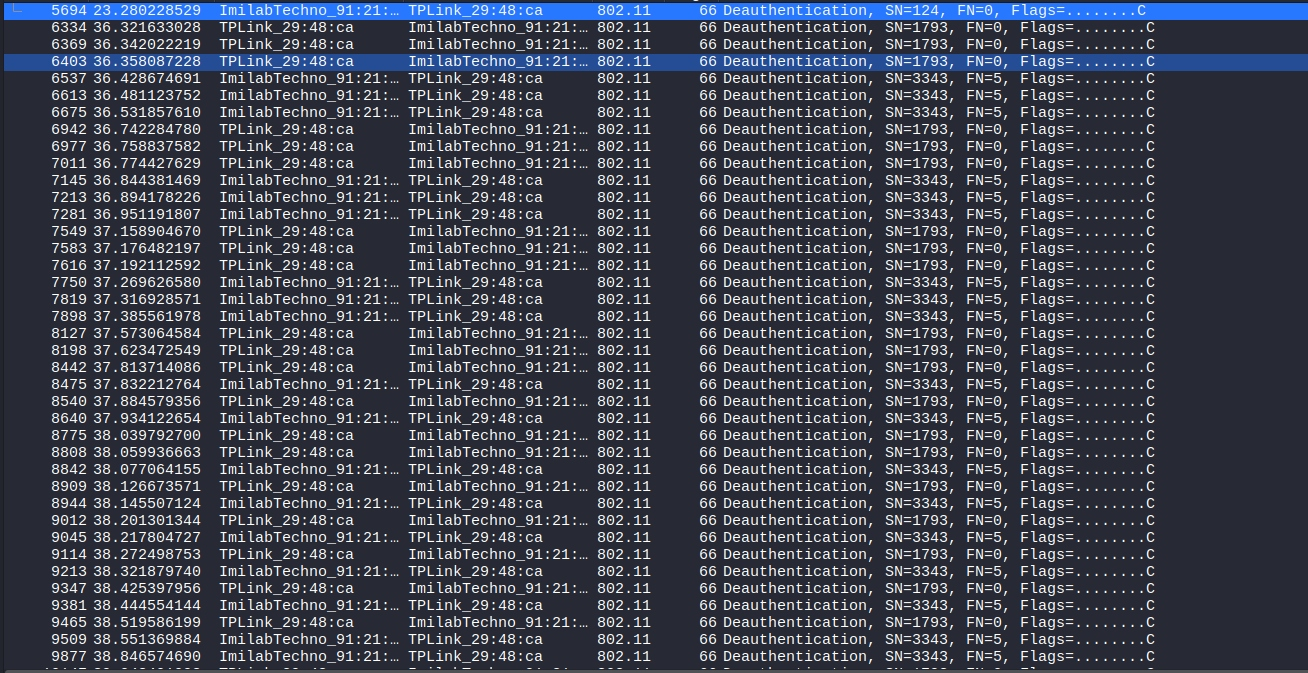
\includegraphics[width=\textwidth]{evidencia_desautenticacao.png}

\legend{Fonte: captura do pesquisador no Wireshark (2026).}

\end{figure}

\begin{table}[htbp]
\centering
\caption{Quadros de desautenticação representativos do ensaio piloto}
\label{tab:seis-registros}
\small
\begin{tabular}{|>{\raggedright\arraybackslash}p{0.16\textwidth}|>{\raggedright\arraybackslash}p{0.26\textwidth}|>{\raggedright\arraybackslash}p{0.32\textwidth}|>{\raggedright\arraybackslash}p{0.12\textwidth}|}
\hline
\textbf{Quadro} & \textbf{Tempo relativo (s)} & \textbf{Sentido lógico} & \textbf{\textit{Reason code}} \\ \hline
19227 & 75,007 & AP-01 $\rightarrow$ CAM-01 & 7 \\ \hline
19494 & 75,163 & CAM-01 $\rightarrow$ AP-01 & 7 \\ \hline
31997 & 83,825 & CAM-01 $\rightarrow$ AP-01 & 7 \\ \hline
32128 & 83,927 & AP-01 $\rightarrow$ CAM-01 & 7 \\ \hline
43822 & 92,127 & CAM-01 $\rightarrow$ AP-01 & 7 \\ \hline
44528 & 92,614 & AP-01 $\rightarrow$ \textit{Broadcast} & 7 \\ \hline
\end{tabular}
\legend{Fonte: elaborado pelo autor a partir do arquivo \texttt{PILOTO\_CAM\_C1\_01.pcapng} (2026).}
\end{table}

\begin{figure}[htbp]\centering

\caption{Impacto do ataque de desautenticação sobre o fluxo de dados da câmera}

\label{fig:impacto_deauth_camera}

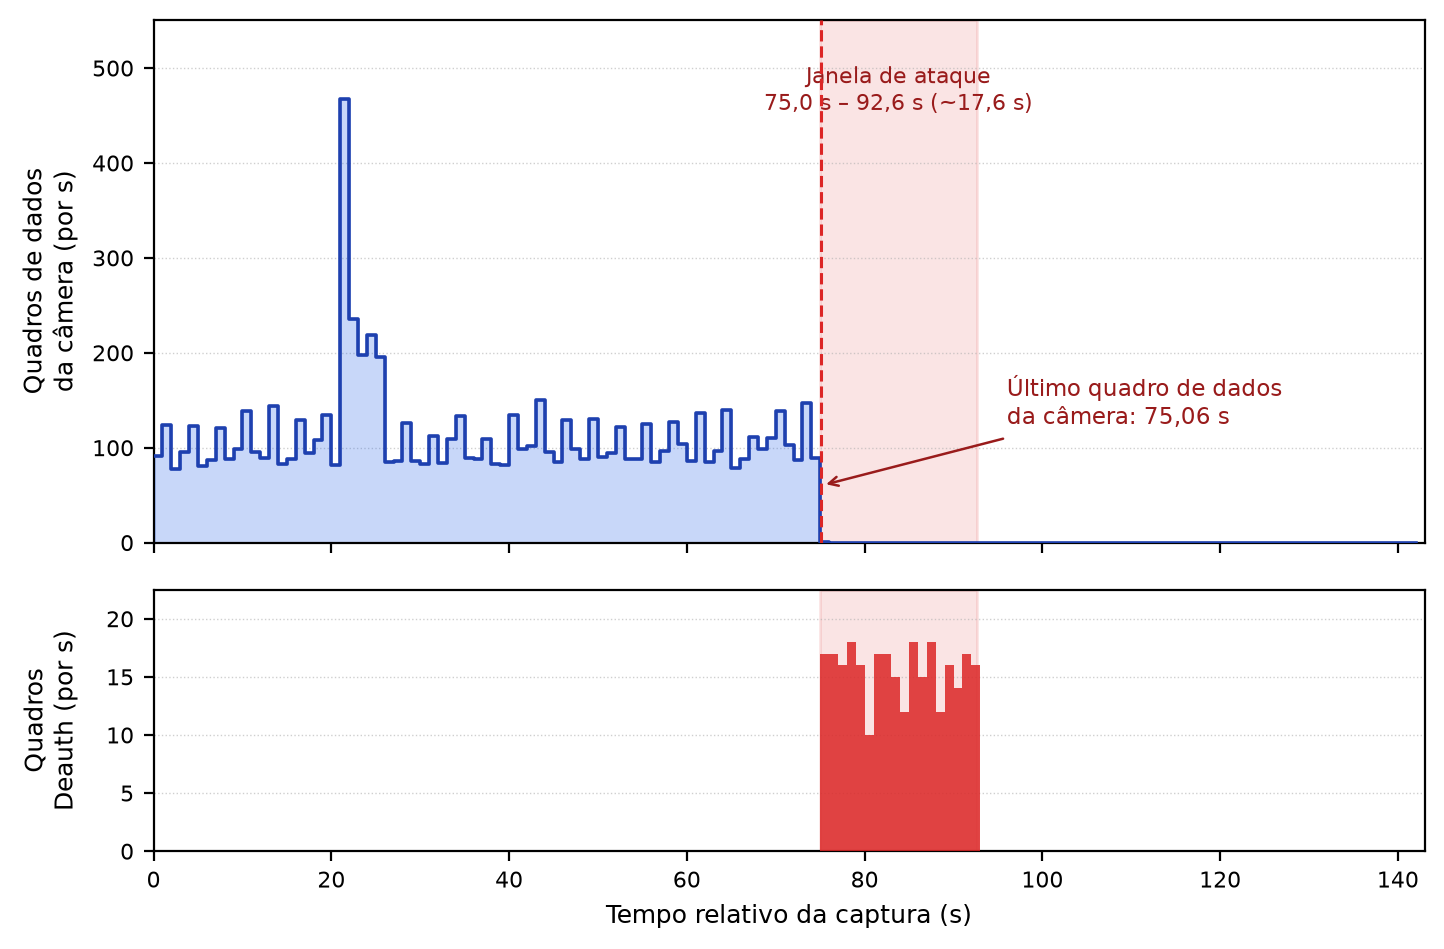
\includegraphics[width=\textwidth]{impacto_deauth_camera.png}

\legend{Fonte: elaborado pelo autor a partir do arquivo \texttt{PILOTO\_CAM\_C1\_01.pcapng} (2026). O painel superior mostra os quadros de dados da câmera por segundo; o inferior, os quadros de desautenticação por segundo. A região sombreada indica a janela de emissão do ataque.}

\end{figure}

\subsection{Desempenho e tempos}

Com a análise dos arquivos de captura, parte dos indicadores de desempenho previstos na metodologia pôde ser efetivamente mensurada nesta etapa, conforme consolidado no Quadro~\ref{quad:situacao-metricas-ref} e na Tabela~\ref{tab:metricas-piloto}. Foram calculados, a partir do arquivo do ensaio piloto, o total de quadros (46.093), o número de quadros de desautenticação (281), a duração da captura (143,0~s), a janela e a taxa de emissão do ataque ($\approx$17,6~s a $\approx$16 quadros/s) e o instante de interrupção do fluxo de dados da câmera (75,06~s), que não voltou a transmitir dados até o fim da captura.

Não foram mensurados, entretanto, o tempo de recuperação funcional do vídeo e o tempo de reassociação do dispositivo no ensaio piloto. O primeiro dependeria de registro sincronizado por \textit{ping} ou por cronômetro, não realizado nesse ensaio; o segundo não pôde ser obtido porque a câmera não se reassociou dentro da janela capturada, tendo sido restabelecida apenas por reinício manual após o encerramento da captura. Esses valores não são estimados por substituição.

\subsection{Segurança negociada por dispositivo}
\label{subsec:consolidacao_resultados}

Após o ensaio piloto com a câmera, o estudo foi estendido ao conjunto completo de dispositivos previsto na metodologia --- câmera IP, lâmpada inteligente, tomada inteligente e \textit{smartphone} de referência ---, em dois cenários de segurança: WPA2 (modo WPA2-PSK[AES]) e um cenário com WPA3 habilitado no roteador em modo misto (WPA2-PSK[AES]+WPA3-Personal), conforme a configuração apresentada na Figura~\ref{fig:painel_roteador_wpa3}. Para cada ensaio foram registrados, de forma sincronizada, o arquivo de captura (gravado pelo \textit{tcpdump} com o adaptador em modo monitor e analisado posteriormente com o \textit{tshark}) e um \textit{log} de \textit{ping} com marcas de tempo (intervalo de 0,5~s), permitindo medir diretamente o tempo de indisponibilidade de cada dispositivo. No cenário WPA2, foram realizadas três repetições independentes para a tomada, a lâmpada e o \textit{smartphone} e duas para a câmera com \textit{ping} (\texttt{CAM\_WPA2\_R03} e \texttt{CAM\_WPA2\_R04}), além do ensaio piloto descrito anteriormente, que não teve \textit{ping}. Uma terceira execução (\texttt{CAM\_WPA2\_R08}) tem linha de base sem ataque, mas o \textit{log} de \textit{ping} apresentou avisos de retrocesso do relógio; por isso, a sua descrição usa os quadros de dados da captura, medida que não foi validada, pois na R03 os dados da câmera não mostram a indisponibilidade observada pelo \textit{ping}. Essa execução é descritiva e não entra nas médias. As execuções \texttt{CAM\_WPA2\_R05} e \texttt{CAM\_WPA2\_R06} foram invalidadas, porque não houve linha de base com respostas normais ao \textit{ping} antes do primeiro quadro de desautenticação direcionado à câmera (Seção~\ref{sec:criterios_validacao}); nenhuma delas entra nas médias. Nas duas execuções da câmera, a função só foi restabelecida após reinício manual; na segunda, o reinício foi feito com a captura em andamento, para registrar o tempo de retorno. No cenário em modo misto, foi realizada uma execução por dispositivo, com duas exceções: a câmera, cujos dois ensaios com \textit{ping} (os arquivos \texttt{CAM\_WPA2\_R02} e \texttt{CAM\_WPA3\_R01}) foram gravados com o ponto de acesso em modo misto; e o \textit{smartphone}, com duas execuções válidas. Nas combinações com uma única execução, cada valor descreve apenas aquela execução e não permite estimar a variação entre repetições. A Tabela~\ref{tab:consolidacao-resultados} consolida os resultados, e a Tabela~\ref{tab:negociacao-seguranca} documenta a segurança negociada por cada dispositivo, obtida do elemento RSN dos quadros de associação nas capturas (Apêndice~\ref{sec:evidencias-rsn}).

Cabe registrar uma restrição de \textit{hardware} relevante para o escopo dos testes. Tanto o microcontrolador LILYGO T-Embed CC1101 Plus, baseado no ESP32-S3 (SoC com dois núcleos Xtensa LX7 e Wi-Fi IEEE~802.11 b/g/n somente em 2,4~GHz, distinto do ESP32 original, de núcleos LX6) \cite{EspressifS3Datasheet}, quanto o adaptador de captura Qualcomm Atheros AR9271 operam exclusivamente na faixa de 2,4~GHz (IEEE 802.11 b/g/n), pois seu \textit{front-end} de rádio não contempla a faixa de 5~GHz. O rádio Wi-Fi do ESP32-S3 é monobanda em 2,4~GHz, de modo que o \textit{firmware} Bruce só consegue injetar quadros de desautenticação nessa faixa; de forma análoga, o AR9271, em modo monitor, só captura tráfego em 2,4~GHz. Por isso, o \textit{smartphone} de referência (Samsung Galaxy S21), inicialmente associado à rede em 5~GHz (canal 157), precisou ser forçado à banda de 2,4~GHz --- desabilitando-se a direção de banda (\textit{band steering}) no roteador --- para ser incluído nos ensaios. Essa restrição é, a um só tempo, uma limitação do estudo e uma observação de segurança: dispositivos que operam exclusivamente em 5~GHz ficam fora do alcance desta plataforma de ataque de baixo custo, baseada em ESP32-S3. A restrição de faixa não se confunde com a segurança negociada: operar em 2,4~GHz não impede o uso de WPA3 ou de PMF, como mostra a própria lâmpada avaliada (Apêndice~\ref{sec:evidencias-rsn}).

Um aspecto determinante para a interpretação dos resultados foi verificado nos quadros de gerenciamento: no cenário em modo misto, cada dispositivo negocia a segurança que suporta, e a configuração exibida no painel do roteador (Figura~\ref{fig:painel_roteador_wpa3}) informa apenas o que o ponto de acesso oferece. Nesse cenário, os \textit{beacons} anunciam os AKM~2 (PSK) e~8 (SAE), com MFPC~=~1 e MFPR~=~0, isto é, PMF oferecido de forma opcional. O campo \textit{Authentication algorithm} do quadro de autenticação não foi tomado como evidência, pois o valor 0 (\textit{Open System}) precede tanto o WPA2-PSK sem PMF quanto o WPA2-PSK com PMF; a evidência adotada é o elemento RSN do \textit{Association Request}, que informa o AKM selecionado e os bits MFPC e MFPR da estação. Por esse critério, a câmera e a tomada selecionaram o AKM~2 (PSK) com MFPC~=~0 e MFPR~=~0, de modo que o PMF não foi negociado, embora oferecido pelo ponto de acesso. A lâmpada, em captura dedicada feita após o seu reinício, realizou a troca SAE (\textit{authentication algorithm}~3) e selecionou o AKM~8 (SAE) com MFPC~=~1 e MFPR~=~1. Para o \textit{smartphone}, que permaneceu associado durante todas as capturas do cenário misto, nenhum quadro de autenticação ou associação foi registrado, e o AKM selecionado não pôde ser observado (AKM não observado); há apenas o indício indireto de que os quadros de gerenciamento do tipo \textit{Action} trocados com o ponto de acesso tinham o bit \textit{Protected} ativo, compatível com PMF negociado, mas incapaz de distinguir SAE de PSK com PMF. Os números dos quadros e os campos de cada evidência constam do Apêndice~\ref{sec:evidencias-rsn}.

\begin{figure}[htb]
\centering
\caption{Configuração da rede em modo misto WPA2/WPA3 no painel do roteador}
\label{fig:painel_roteador_wpa3}
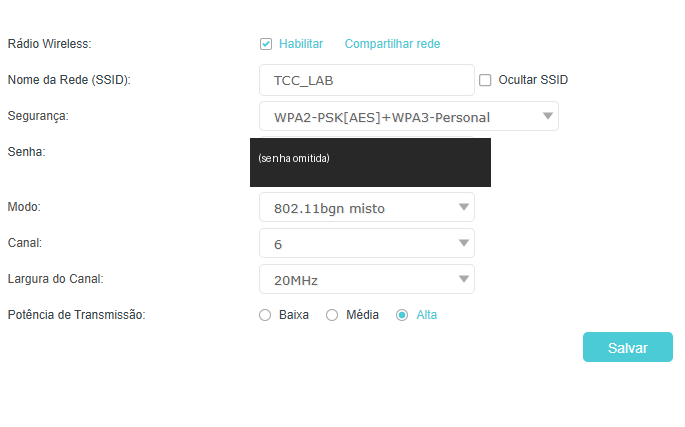
\includegraphics[width=0.82\textwidth]{painel_roteador_wpa3.png}
\legend{Fonte: captura do pesquisador no painel administrativo do TP-Link EX1500 (2026). A senha foi omitida.}
\end{figure}

\begin{table}[htbp]
\centering
\caption[Segurança negociada por dispositivo (modo misto)]{Segurança negociada por cada dispositivo no cenário misto WPA2/WPA3}
\label{tab:negociacao-seguranca}
\marcadoresTabela
\small
\begin{tabular}{|>{\raggedright\arraybackslash}p{0.19\textwidth}|>{\raggedright\arraybackslash}p{0.17\textwidth}|>{\raggedright\arraybackslash}p{0.17\textwidth}|>{\raggedright\arraybackslash}p{0.14\textwidth}|>{\raggedright\arraybackslash}p{0.20\textwidth}|}
\hline
\textbf{Dispositivo} & \textbf{AKM selecionado} & \textbf{MFPC / MFPR (estação)} & \textbf{PMF negociado} & \textbf{Perda de associação observada} \\ \hline
Câmera IP & 2 (PSK) & 0 / 0 & Não & Sim (em 1 de 2 execuções) \\ \hline
Tomada inteligente & 2 (PSK) & 0 / 0 & Não & Sim \\ \hline
Lâmpada inteligente & 8 (SAE)\textsuperscript{a} & 1 / 1 & Sim & Não \\ \hline
\textit{Smartphone} (ref.) & Não observado\textsuperscript{b} & Não observado & Indício indireto\textsuperscript{b} & Não (manteve a associação) \\ \hline
\end{tabular}
\legend{Fonte: elaborado pelo autor a partir do elemento RSN dos quadros de \textit{Association Request} nas capturas (2026); números dos quadros no Apêndice~\ref{sec:evidencias-rsn}. Ponto de acesso no cenário misto: AKM~2 e~8, MFPC~=~1, MFPR~=~0. ``Perda de associação observada'': presença de novas autenticações e associações da estação na captura do ensaio. \textsuperscript{a}Obtido em captura dedicada, após o reinício da lâmpada, e não durante o ensaio de ataque. \textsuperscript{b}Nenhuma associação do \textit{smartphone} foi capturada no cenário misto; quadros de gerenciamento \textit{Action} com o bit \textit{Protected} ativo indicam PMF, sem identificar o AKM. Manter a associação não significa ausência de impacto: o \textit{smartphone} registrou intervalos sem resposta a \textit{ping} (Figura~\ref{fig:comparacao_pmf}).}
\end{table}

A Tabela~\ref{tab:negociacao-seguranca} mostra que a coluna decisiva é a do PMF negociado, e não o rótulo do cenário: câmera e tomada, que não declaram MFPC, operaram sem PMF mesmo com o ponto de acesso oferecendo-o; a tomada e a câmera, em uma das duas execuções (\texttt{CAM\_WPA3\_R01}), apresentaram novas autenticações e associações durante o ataque; a lâmpada, com PMF obrigatório, e o \textit{smartphone}, com indício indireto de PMF, mantiveram a associação. Para o \textit{smartphone}, a última coluna registra apenas a manutenção da associação, e não proteção completa, pois houve intervalos sem resposta a \textit{ping}.

\subsection{Consolidação dos resultados por dispositivo e cenário}
\label{subsec:consolidacao_tabelas}

Os resultados consolidados estão divididos em duas tabelas, para que cada linha informe o número de execuções ($n$) que a sustenta. A Tabela~\ref{tab:consolidacao-resultados} reúne os indicadores de conectividade: a quantidade de quadros de desautenticação direcionados ao dispositivo e o tempo acumulado sem resposta a \textit{ping}, conforme definido na Seção~\ref{subsec:dicionario_metricas}. Nas linhas com uma única execução, o número exibido é o valor observado nessa execução, e não uma média; nas linhas com mais de uma execução, são apresentados os valores individuais, a média e a amplitude (diferença entre o maior e o menor valor), exceto quando algum valor é limite inferior ($\geq$), caso em que a média não é calculada. Os valores de cada execução, com a respectiva janela de ataque, constam das Tabelas~\ref{tab:registro-execucoes} e~\ref{tab:registro-metricas}.

\renewcommand{\arraystretch}{1.2}
\begin{table}[htbp]
\centering
\caption{Consolidação dos resultados por dispositivo e cenário: conectividade}
\label{tab:consolidacao-resultados}
\marcadoresTabela
\scriptsize
\setlength{\tabcolsep}{2.5pt}
\begin{tabular}{|>{\raggedright\arraybackslash}p{0.11\textwidth}|>{\raggedright\arraybackslash}p{0.075\textwidth}|>{\raggedright\arraybackslash}p{0.05\textwidth}|>{\raggedright\arraybackslash}p{0.09\textwidth}|>{\raggedright\arraybackslash}p{0.09\textwidth}|>{\raggedright\arraybackslash}p{0.09\textwidth}|>{\raggedright\arraybackslash}p{0.09\textwidth}|>{\raggedright\arraybackslash}p{0.10\textwidth}|>{\raggedright\arraybackslash}p{0.10\textwidth}|}
\hline
\textbf{Dispositivo} & \textbf{Cenário} & \textbf{$n$} & \textbf{Deauth no disp.} & \multicolumn{3}{>{\centering\arraybackslash}p{0.28\textwidth}|}{\textbf{Tempo acumulado sem resposta por execução (s)}} & \textbf{Média ou valor observado (s)} & \textbf{Amplitude (s)} \\ \cline{5-7}
 & & & & \textbf{R01} & \textbf{R02} & \textbf{R03} & & \\ \hline
Câmera IP & WPA2 & 2 & 625,5 (média) & \multicolumn{3}{c|}{R03: $\geq$160,1; R04: 82,4} & não calculada\textsuperscript{d} & --- \\ \hline
Câmera IP & misto\textsuperscript{a} & 2 & 519,5 (média) & $\geq$55,8 & $\geq$56,5 & --- & não calculada\textsuperscript{a} & --- \\ \hline
Tomada & WPA2 & 3 & 467 (média) & $\geq$45,4\textsuperscript{b} & 106,4 & 93,6 & não calculada\textsuperscript{b} & --- \\ \hline
Tomada & misto & 1 & 712 & \multicolumn{3}{c|}{execução única} & 72,5 (observado) & --- \\ \hline
Lâmpada & WPA2 & 3 & 405 (média) & 40,1 & 49,4 & 52,8 & 47,4 (média) & 12,7 \\ \hline
Lâmpada & misto & 1 & 425 & \multicolumn{3}{c|}{execução única} & 0,0 (observado) & --- \\ \hline
\textit{Smartphone} & WPA2 & 3 & 502 (média) & 73,1 & 66,5 & 65,3 & 68,3 (média) & 7,8 \\ \hline
\textit{Smartphone} & misto\textsuperscript{c} & 2 & 578 (média) & 22,8 & inválida & 24,7 & 23,8 (média) & 1,9 \\ \hline
\end{tabular}
\legend{Fonte: elaborado pelo autor a partir dos arquivos de captura e dos \textit{logs} de \textit{ping} (2026). ``Misto'': WPA3 habilitado em modo misto (WPA2-PSK[AES]+WPA3-Personal). ``Deauth no disp.'': quadros de desautenticação com o endereço do dispositivo como origem ou destino (média das execuções, nas linhas com $n>1$). Tempo acumulado sem resposta: soma dos intervalos sem resposta a \textit{ping} acima de 2~s, excluídas as respostas duplicadas (\textit{DUP!}). A câmera em WPA2 teve duas execuções com \textit{ping} (\texttt{CAM\_WPA2\_R03} e \texttt{CAM\_WPA2\_R04}, nota d); o ensaio piloto não teve \textit{ping} (Tabela~\ref{tab:metricas-piloto}). \textsuperscript{a}As duas execuções da câmera em modo misto correspondem aos arquivos \texttt{CAM\_WPA2\_R02} ($\geq$55,8~s, sem reassociação, exigiu reinício manual) e \texttt{CAM\_WPA3\_R01} ($\geq$56,5~s, com reassociações durante o ataque, mas sem resposta válida a \textit{ping} até o fim da captura; reiniciada manualmente após o fim da captura, com retorno não registrado); em ambos o AP anunciava modo misto e a câmera negociou PSK sem PMF (Apêndice~\ref{sec:evidencias-rsn}). Nas duas execuções, a queda vai até o encerramento da captura, de modo que os valores são limites inferiores e a média não é calculada. \textsuperscript{b}A execução \texttt{TOMADA\_WPA2\_R01} foi registrada com intervalo de \textit{ping} de 1~s (as demais, 0,5~s) e com menor número de quadros de desautenticação direcionados à tomada (49, contra 843 e 510); a última resposta válida ocorreu aos 104,8~s do \textit{log}, e o \textit{ping} prosseguiu sem resposta válida até o fim da captura, enquanto a tomada se reassociava repetidamente; por isso o valor é limite inferior e a média não é calculada. \textsuperscript{c}O \textit{smartphone} em modo misto teve a execução \texttt{PHONE\_WPA3\_R02} invalidada por não conter quadros de desautenticação direcionados a ele (Seção~\ref{sec:criterios_validacao}); a média usa as duas execuções válidas (\texttt{R01} e \texttt{R03}). \textsuperscript{d}Câmera em WPA2: \texttt{CAM\_WPA2\_R03} não teve associação da câmera registrada na captura; o último \textit{ping} válido ocorreu aos 94,9~s da captura, e o intervalo sem resposta termina apenas com o encerramento da captura, aos 254,9~s, por isso o valor é um limite inferior ($\geq$160~s). O reinício foi feito depois desse encerramento. \texttt{CAM\_WPA2\_R04} teve oito trocas de autenticação e associação durante o ataque (entre 88,6 e 95,5~s, todas com \textit{status} 0), cada uma seguida de novo quadro de desautenticação, e uma nova associação após o reinício (184,5~s); o tempo sem resposta forma uma única queda contínua de 82,4~s, calculada sobre respostas válidas. Os \textit{logs} de \textit{ping} das duas execuções registram avisos de retrocesso do relógio, após os quais aparecem apenas linhas \texttt{icmp\_seq=0 (DUP!)}, excluídas do cálculo. A média não é calculada porque um dos valores é limite inferior. A execução \texttt{CAM\_WPA2\_R05} foi invalidada (Seção~\ref{sec:criterios_validacao}) e não entra nesta tabela (Tabelas~\ref{tab:registro-execucoes} e~\ref{tab:registro-metricas}, nota i). A execução \texttt{CAM\_WPA2\_R08}, medida pela captura porque o \textit{log} de \textit{ping} não é confiável, também não entra nas médias por \textit{ping} (Tabelas~\ref{tab:registro-execucoes} e~\ref{tab:registro-metricas}, nota j).}
\end{table}

A Tabela~\ref{tab:consolidacao-recuperacao} complementa a anterior com os indicadores de recuperação: a maior queda contínua, a forma de recuperação da rede e da função do dispositivo, a necessidade de intervenção manual e o resultado de cada combinação de dispositivo e cenário, segundo as quatro categorias definidas na metodologia. A separação entre recuperação de rede e recuperação da função é necessária porque o retorno das respostas a \textit{ping} não garante que a imagem da câmera ou o comando da tomada e da lâmpada tenham voltado a funcionar.

\begin{table}[htbp]
\centering
\caption{Consolidação dos resultados por dispositivo e cenário: recuperação}
\label{tab:consolidacao-recuperacao}
\marcadoresTabela
\scriptsize
\setlength{\tabcolsep}{3pt}
\begin{tabular}{|>{\raggedright\arraybackslash}p{0.115\textwidth}|>{\raggedright\arraybackslash}p{0.08\textwidth}|>{\raggedright\arraybackslash}p{0.035\textwidth}|>{\raggedright\arraybackslash}p{0.118\textwidth}|>{\raggedright\arraybackslash}p{0.15\textwidth}|>{\raggedright\arraybackslash}p{0.13\textwidth}|>{\raggedright\arraybackslash}p{0.075\textwidth}|>{\raggedright\arraybackslash}p{0.17\textwidth}|}
\hline
\textbf{Dispositivo} & \textbf{Cenário} & \textbf{$n$} & \textbf{Maior queda contínua (s)} & \textbf{Recuperação de rede} & \textbf{Recuperação da função} & \textbf{Interv. manual} & \textbf{Resultado} \\ \hline
Câmera IP & WPA2 & 2 & $\geq$160 (R03); 82,4 (R04) & não observada até o fim da captura (R03); retorno só após reinício manual (R04) & não mensurada & Sim em 2 de 2 & Desassociação confirmada em R04; não confirmada em R03 (ver Tabela~\ref{tab:consolidacao-resultados}) \\ \hline
Câmera IP & misto & 2 & $\geq$55,8 e $\geq$51,3 & não espontânea (\texttt{CAM\_\allowbreak{}WPA2\_\allowbreak{}R02}) / não observada até o fim da captura (\texttt{CAM\_\allowbreak{}WPA3\_\allowbreak{}R01}) & não mensurada & Sim em 2 de 2\textsuperscript{a} & Desassociação confirmada em \texttt{CAM\_WPA3\_R01}\textsuperscript{a} \\ \hline
Tomada & WPA2 & 3 & $\geq$33,2; 80,7; 48,3 (média não calculada) & automática (intermitente)\textsuperscript{c} & não mensurada & Não & Desassociação confirmada \\ \hline
Tomada & misto & 1 & 63,3 & automática (intermitente) & não mensurada & Não & Desassociação confirmada \\ \hline
Lâmpada & WPA2 & 3 & 47,4 (média) & automática (intermitente) & não mensurada & Não & Desassociação confirmada \\ \hline
Lâmpada & misto & 1 & 0,0 & não afetada & não mensurada & Não & Sem efeito detectado \\ \hline
\textit{Smartphone} & WPA2 & 3 & 65,1 (média) & manual (seleção da rede) & não mensurada & Sim & Desassociação confirmada \\ \hline
\textit{Smartphone} & misto & 2 & 5,5 (média) & não afetada (manteve associação) & não mensurada & Não & Perda de conectividade sem desassociação confirmada\textsuperscript{b} \\ \hline
\end{tabular}
\legend{Fonte: elaborado pelo autor a partir dos arquivos de captura e dos \textit{logs} de \textit{ping} (2026). ``Maior queda contínua'': maior intervalo isolado sem resposta a \textit{ping}; valor médio nas linhas com $n>1$, exceto quando algum valor é limite inferior ($\geq$), caso em que os valores individuais são listados. ``Desassociação confirmada'' foi atribuída quando a captura registra novos quadros de autenticação e de \textit{Association Request} com o endereço do dispositivo durante o ataque; ``recuperação da função'' não foi mensurada por \textit{ping}. \textsuperscript{a}As duas execuções da câmera em modo misto diferiram: em \texttt{CAM\_WPA2\_R02} não houve reassociação na captura (perda de conectividade sem desassociação confirmada; recuperação só por reinício manual), ao passo que em \texttt{CAM\_WPA3\_R01} a câmera reassociou-se várias vezes durante o ataque (desassociação confirmada), mas não voltou a responder a \textit{ping} nem a transmitir quadros de dados até o fim da captura, encerrada 6,8~s após o fim do ataque; a câmera foi reiniciada manualmente após o fim da captura, e o retorno não foi registrado. \textsuperscript{b}O \textit{smartphone} manteve a associação (nenhum quadro de autenticação ou associação dele na captura), mas registrou intervalos sem resposta a \textit{ping}. \textsuperscript{c}Em \texttt{TOMADA\_WPA2\_R01}, a retomada não foi observada até o fim da captura, encerrada logo após o fim do ataque.}
\end{table}
\renewcommand{\arraystretch}{1.0}

A Figura~\ref{fig:comparacao_pmf} sintetiza o achado central do estudo, apresentando, para cada dispositivo e cenário, a fração do tempo sem resposta a \textit{ping} (Seção~\ref{subsec:dicionario_metricas}); a cor indica se o dispositivo negociou ou não o PMF, o hachurado distingue o cenário misto do cenário WPA2 e os pontos sobre cada barra marcam as execuções individuais. Abaixo de cada barra é indicado o número de execuções ($n$); as barras com $n > 1$ mostram a média, e as barras com $n = 1$, o valor observado. As barras marcadas com $\geq$ incluem ao menos uma execução cuja queda durou até o fim da captura; nesses casos, o valor é um limite inferior. Sem PMF, todos os casos apresentaram fração expressiva de tempo sem resposta: no cenário WPA2, de $\approx$43\% (lâmpada) a $\approx$59\% (\textit{smartphone}), com a câmera ($\geq$51\%) e a tomada ($\geq$47\%) representadas por limites inferiores; e no cenário misto, em que câmera e tomada negociaram PSK sem PMF, de $\geq$53\% (câmera, limites inferiores de 56\% e 50\% em duas execuções) a $\approx$71\% (tomada). Com PMF (lâmpada, com PMF obrigatório negociado; \textit{smartphone}, com indício indireto de PMF), a lâmpada não apresentou intervalos sem resposta na janela observada e o \textit{smartphone}, embora tenha mantido a associação, registrou em média $\approx$22\% do tempo sem resposta (14\% e 29\% em duas execuções). Portanto, câmera e tomada permaneceram sem PMF mesmo com o WPA3 habilitado no roteador em modo misto. No cenário WPA2, a câmera aparece na figura com as execuções \texttt{CAM\_WPA2\_R03} ($\geq$63\%, limite inferior) e \texttt{CAM\_WPA2\_R04} ($\approx$38\%); as demais execuções da câmera nesse cenário não entram, pelos motivos indicados nas Tabelas~\ref{tab:consolidacao-resultados} e~\ref{tab:consolidacao-recuperacao}.

\begin{figure}[htb]
\centering
\caption{Tempo sem resposta a \textit{ping} por dispositivo e cenário, com e sem PMF}
\label{fig:comparacao_pmf}
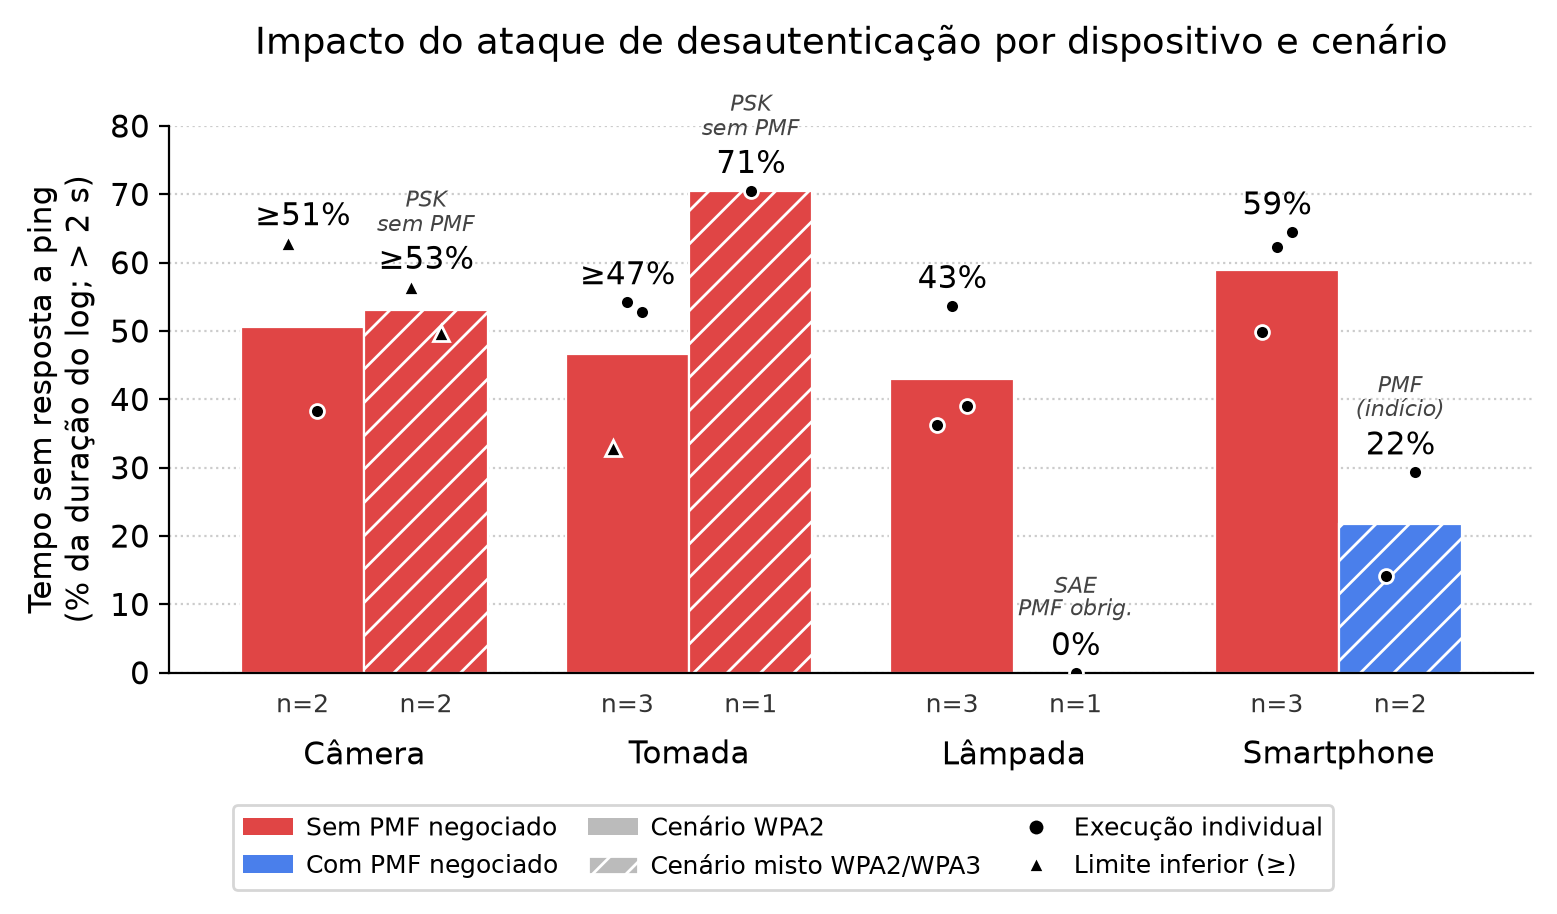
\includegraphics[width=0.95\textwidth]{comparacao_pmf.png}
\legend{Fonte: elaborado pelo autor a partir dos \textit{logs} de \textit{ping} dos ensaios (2026). Eixo vertical: tempo acumulado sem resposta ($>$2~s), excluídas as respostas duplicadas (\textit{DUP!}), dividido pela duração do \textit{log} de \textit{ping}; não equivale à perda de pacotes ICMP. Os pontos indicam as execuções individuais e $n$, o seu número; os triângulos marcam execuções cuja queda durou até o fim da captura. Barras com $\geq$ incluem pelo menos uma execução cuja queda durou até o fim da captura; o valor é um limite inferior da média, e não uma média propriamente dita. No cenário WPA2, a câmera aparece com \texttt{CAM\_WPA2\_R03} e \texttt{CAM\_WPA2\_R04}; \texttt{CAM\_WPA2\_R05} e \texttt{CAM\_WPA2\_R06} (invalidadas) e \texttt{CAM\_WPA2\_R08} (medida pela captura, não por \textit{ping}) não entram. Valores calculados pelo \textit{script} \texttt{src/analisa\_ping.py} e figura gerada por \texttt{src/figura\_comparacao\_pmf.py}. As janelas de ataque de cada execução constam das Tabelas~\ref{tab:registro-execucoes} e~\ref{tab:registro-metricas}.}
\end{figure}

A Figura~\ref{fig:ping_lampada} mostra, para a lâmpada, as respostas a \textit{ping} ao longo de uma execução de cada cenário. No cenário WPA2, em que a lâmpada se associou com PSK e sem PMF, as respostas cessaram pouco depois do início do ataque e só voltaram após o seu término, em um único intervalo de 40,1~s sem resposta. No modo misto, em que a lâmpada negociou SAE com PMF obrigatório, as respostas continuaram durante todo o ataque, sem nenhum intervalo maior que 2~s, embora o tempo de resposta tenha oscilado mais durante a janela de ataque.

\begin{figure}[htb]
\centering
\caption{Respostas a \textit{ping} da lâmpada durante o ataque nos cenários WPA2 e modo misto WPA2/WPA3}
\label{fig:ping_lampada}
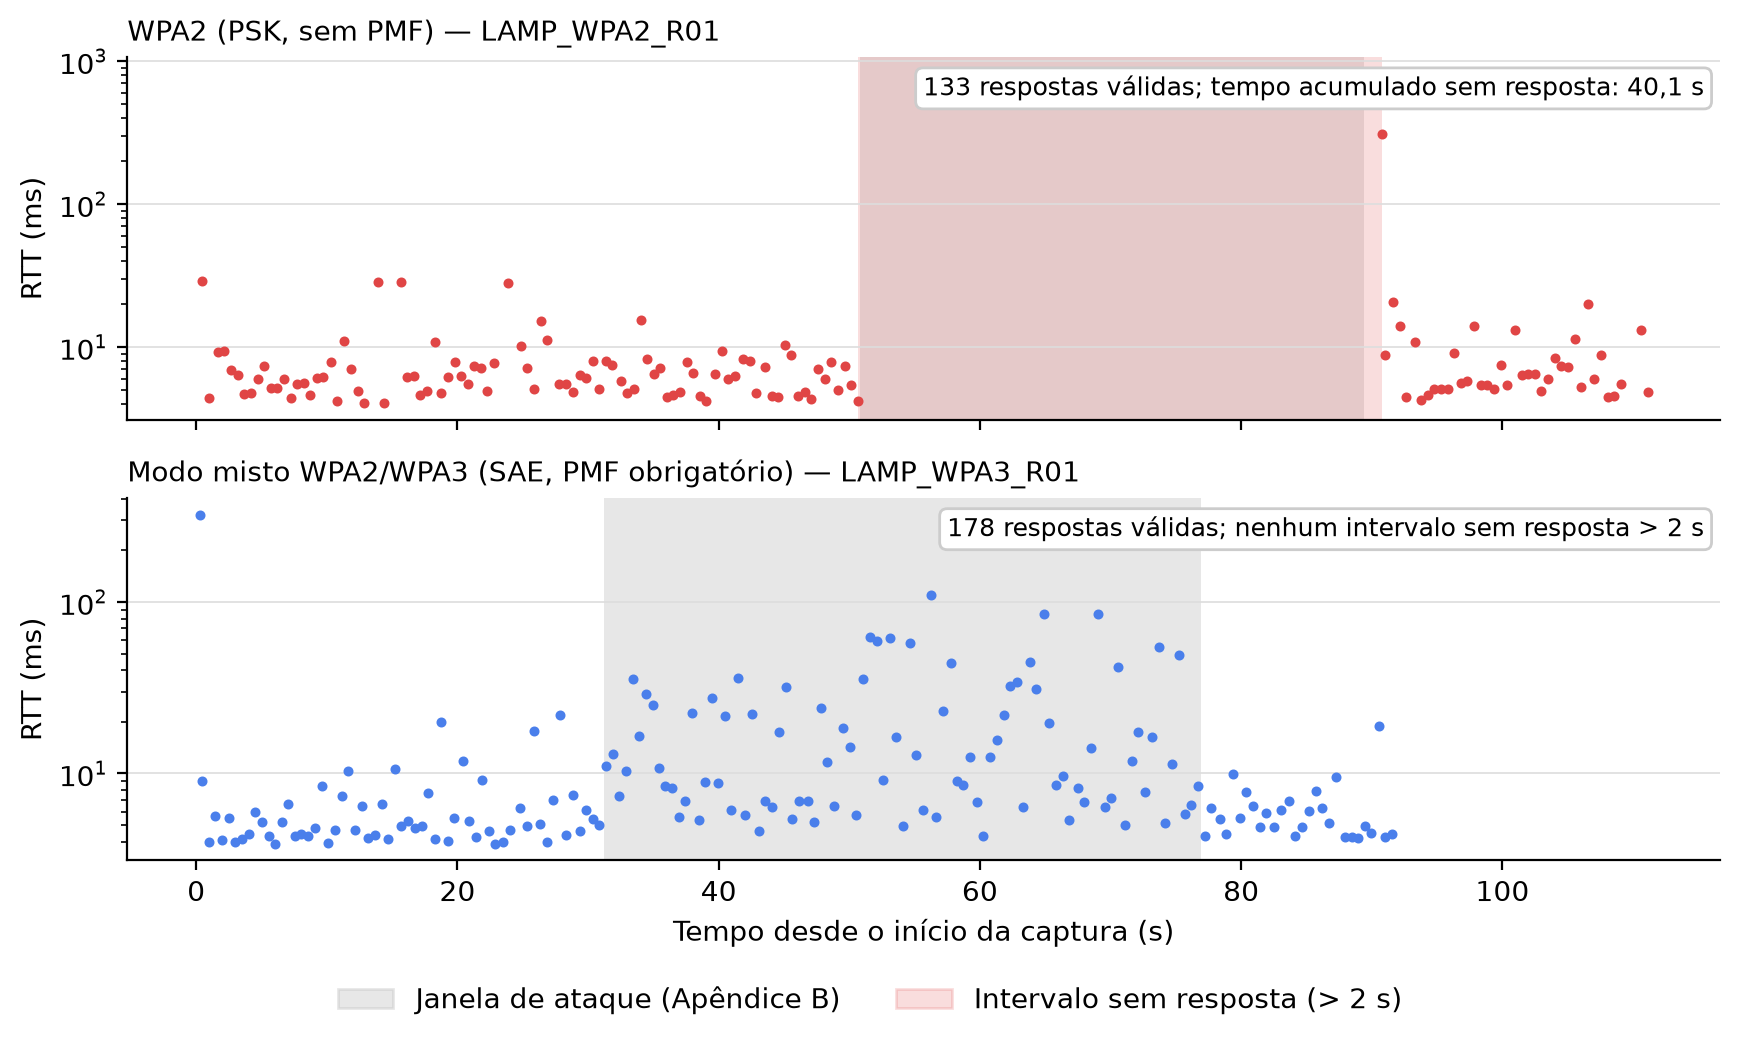
\includegraphics[width=0.95\textwidth]{ping_lampada.png}
\legend{Fonte: elaborado pelo autor a partir dos \textit{logs} de \textit{ping} das execuções \texttt{LAMP\_WPA2\_R01} e \texttt{LAMP\_WPA3\_R01} e do \textit{script} \texttt{src/figura\_ping\_lampada.py} (2026). Cada ponto é uma resposta válida (RTT em escala logarítmica). Faixa cinza: janela de ataque (Apêndice~\ref{sec:registro-execucoes}). Faixa vermelha: intervalo sem resposta maior que 2~s.}
\end{figure}

\subsection{Padrões de comportamento observados}
\label{subsec:padroes}

Os ensaios revelaram três padrões distintos de resposta ao ataque de desautenticação, todos no cenário WPA2 (sem PMF). A \textbf{câmera} interrompeu completamente o fluxo de vídeo. Em \texttt{CAM\_WPA2\_R03} não houve reassociação registrada na captura; em \texttt{CAM\_WPA2\_R04}, ela reassociou-se oito vezes durante o ataque, sempre seguida de nova desautenticação, e não se reassociou após o seu término. Em ambas, a função só foi restabelecida após reinício manual. A \textbf{tomada} e a \textbf{lâmpada} apresentaram um padrão intermitente na camada de enlace: eram desassociadas e reassociavam-se repetidamente durante o ataque (captura), sem voltar a responder ao \textit{ping} de forma estável até o seu término, com recuperação automática depois dele (exceto em \texttt{TOMADA\_WPA2\_R01}, cuja captura terminou antes da retomada). O \textbf{smartphone}, por sua vez, perdeu a conexão e não a restabeleceu sozinho, exibindo uma falsa mensagem de ``senha incorreta'' e só reconectando após intervenção manual do usuário na seleção da rede. Essa diversidade evidencia que o impacto de um mesmo ataque depende não apenas da camada de enlace, mas também da implementação de reconexão de cada dispositivo.

No cenário com WPA3 habilitado em modo misto, observou-se que a segurança é negociada por dispositivo, e não pela rede como um todo. A lâmpada, que negociou SAE com PMF obrigatório, manteve fluxo de dados contínuo e \textit{ping} sem intervalos sem resposta, apesar de 425 quadros de desautenticação a ela direcionados; o \textit{smartphone}, com indício indireto de PMF, manteve a associação mesmo sob mais de 500 quadros por execução nas execuções com ataque ao alvo, embora com intervalos sem resposta a \textit{ping}. Em contraste, a câmera e a tomada, que selecionaram PSK sem declarar suporte a PMF, apresentaram perda de associação e tempos sem resposta da mesma ordem do cenário WPA2; a câmera, como no cenário WPA2, não voltou a responder sem reinício manual, feito nas duas execuções. Esse padrão é compatível com a proteção esperada dos quadros de gerenciamento e indica que habilitar o WPA3 em modo misto não altera a exposição dos dispositivos IoT legados ao ataque de desautenticação.

\section{Discussão dos resultados}
\label{sec:discussao}

\subsection{Comparação entre o esperado e o obtido}

O referencial teórico discute a desautenticação como um mecanismo relacionado ao estado de autenticação e associação de estações, bem como os riscos de quadros de gerenciamento falsificados quando não há proteção apropriada. A identificação desse tipo de quadro no ensaio é coerente com o mecanismo investigado, porém não demonstra, por si só, quebra da criptografia de dados ou comprometimento de credenciais \cite{KohliosHayajneh2018}.



A comparação com o estudo de \citeonline{KristiyantoErnastuti2020}, já apresentado no referencial, deve preservar a diferença entre semelhança do arranjo experimental e equivalência de resultados. Ambos os recortes envolvem câmera IP, ponto de acesso e microcontrolador como instrumento de teste, e ambos confirmam a eficácia do ataque de desautenticação contra dispositivos IoT. Entretanto, os valores absolutos de indisponibilidade não são diretamente comparáveis, pois dependem do \textit{firmware}, da distância e da intensidade do ataque; a contribuição adicional deste trabalho está no registro, por dispositivo, da segurança efetivamente negociada (AKM e PMF) ao lado do impacto do ataque. Essa comparação não isola o efeito de um único fator: entre os dispositivos que mantiveram a associação e os que a perderam variaram, em conjunto, o AKM (SAE ou PSK), o PMF, o fabricante, o \textit{firmware} e a lógica de reconexão de cada equipamento. O resultado é, portanto, um padrão compatível com a proteção esperada dos quadros de gerenciamento pelo PMF, e não uma demonstração de causalidade exclusiva.



Em relação ao esperado, os objetivos específicos 1 e 2 foram atendidos, e os objetivos 3 e 4, parcialmente, conforme detalhado na Seção~\ref{sec:atendimento_objetivos}. O ambiente de ataque foi configurado e validado; os testes de desautenticação foram executados contra os quatro dispositivos; os tempos de indisponibilidade foram mensurados por \textit{ping} sincronizado, com três repetições para a tomada, a lâmpada e o \textit{smartphone} no cenário WPA2; e os dados de tráfego foram coletados e analisados para validar a eficácia técnica dos testes. A comparação entre os mecanismos de proteção foi realizada e mostrou que o rótulo configurado no roteador (WPA2 ou modo misto) não descreve, por si só, a situação de cada dispositivo: os dispositivos que operaram sem PMF apresentaram perda de conectividade em todos os ensaios --- com desassociação confirmada por novos quadros de autenticação e associação na maioria deles, exceto nas execuções \texttt{CAM\_WPA2\_R02} e \texttt{CAM\_WPA2\_R03}, em que a câmera não se reassociou e a desassociação não pôde ser confirmada pela captura ---, ao passo que a lâmpada, com SAE e PMF obrigatório, e o \textit{smartphone}, com indício indireto de PMF, mantiveram a associação. Esse padrão é compatível com a proteção esperada dos quadros de gerenciamento, mas, como SAE, PMF e o próprio dispositivo variaram juntos e não houve condição de WPA2 com PMF, não permite atribuir o resultado exclusivamente ao PMF.

O \textit{smartphone}, embora tenha mantido a associação no cenário misto, registrou em média $\approx$22\% do tempo sem resposta a \textit{ping} (14\% e 29\% em duas execuções). Uma hipótese para essa perda residual é a ocupação do canal pela emissão contínua de quadros de desautenticação, que compete pelo meio com o tráfego do dispositivo; outras explicações possíveis são a economia de energia do sistema operacional do \textit{smartphone} e perdas de recepção. Essas hipóteses não foram testadas neste trabalho, pois não se mediu a ocupação do canal nem se repetiu o ensaio sem o ataque nas mesmas condições.



A contribuição deste estudo consiste em demonstrar, de forma prática e mensurada, que uma plataforma de baixo custo (LILYGO T-Embed CC1101 Plus com \textit{firmware} Bruce) é capaz de desconectar dispositivos IoT comerciais por meio de ataques de desautenticação em redes IEEE 802.11 sem PMF, e em registrar que apenas os dispositivos que negociaram PMF mantiveram a associação, padrão compatível com a proteção esperada dos quadros de gerenciamento. Não se reivindica generalização para todos os roteadores, dispositivos ou \textit{firmwares} existentes, dado o caráter de estudo de caso com amostra intencional.

\subsection{Cenário crítico de aplicação: monitoramento de câmaras de vacinas}
\label{subsec:cenario_vacinas}

Esta subseção não relata um ensaio. Nenhum equipamento de monitoramento de vacinas foi testado na bancada: trata-se de uma análise de impacto que transporta os resultados medidos neste trabalho para um contexto em que a perda de disponibilidade da rede teria consequências maiores do que nos dispositivos residenciais avaliados. As fontes sobre monitoramento de vacinas citadas a seguir não tratam de ataques à rede sem fio; a ligação entre esse contexto e o ataque de desautenticação é uma inferência deste trabalho, apoiada nos resultados da bancada e no referencial sobre o IEEE~802.11.

Na Rede de Frio do Programa Nacional de Imunizações (PNI), as câmaras científicas refrigeradas usadas na conservação de imunobiológicos são projetadas para armazená-los entre 2~\textdegree{}C e 8~\textdegree{}C (BRASIL, \citeyear{BrasilRedeFrio2025}, p.~61). Para acompanhar essa faixa, a literatura descreve sistemas de monitoramento baseados em microcontroladores com Wi-Fi, que enviam as leituras de temperatura a serviços em nuvem e emitem alertas remotos. \citeonline{Harrabi2024} empregaram um ESP32, da mesma família de SoCs da Espressif que o ESP32-S3 usado como plataforma de ataque neste trabalho, para monitorar a temperatura de refrigeradores de vacinas, transmitir os dados sem fio e enviar alertas a um aplicativo de celular em situações como falha do sensor, queda de energia e porta aberta. \citeonline{PoochayaWidjaja2018} descrevem um sistema baseado em Wi-Fi e IoT que avisa o farmacêutico quando o refrigerador sai da faixa de temperatura, e \citeonline{Adilah2025} combinam um ESP32 com armazenamento em nuvem, registro em cartão de memória local e alertas por aplicativo de mensagens, avaliados em uma câmara fria real. No contexto brasileiro, \citeonline{Barbosa2022} relata casos de doses descartadas por oscilação de temperatura e propõe um dispositivo IoT para monitorar a temperatura das vacinas em campanhas de vacinação extramuros, e \citeonline{SilvaSantos2023} desenvolveram uma aplicação de monitoramento em tempo real, com registro histórico e alertas de temperatura, voltada à Rede de Frio do PNI.

Nesses sistemas, convém separar a função local, de refrigeração, da função de rede, de telemetria e alarme remoto. O ataque de desautenticação atua sobre a segunda: afeta a disponibilidade da comunicação entre o sensor e o ponto de acesso \cite{KohliosHayajneh2018}, mas não desliga o compressor nem altera a temperatura interna. Durante o ataque, a refrigeração continuaria funcionando; o que se perderia seriam o envio das leituras e o alarme remoto.

Os resultados medidos indicam como essa perda poderia ocorrer. Nas condições estudadas, os dispositivos associados sem PMF perderam a conectividade enquanto o ataque estava ativo (Figura~\ref{fig:comparacao_pmf}). No cenário WPA2, a tomada ficou sem responder a \textit{ping} por $\geq$45,4~s, 106,4~s e 93,6~s (o primeiro valor é limite inferior), e a lâmpada, por 40,1~s a 52,8~s ($n=3$ cada); ambas se reassociaram repetidamente durante o ataque e voltaram a responder de forma automática depois do seu término, exceto em uma execução da tomada, cuja captura terminou antes da retomada (Seção~\ref{subsec:padroes}). A câmera teve o comportamento mais grave para um cenário de monitoramento: não recuperou a conectividade sozinha em nenhuma das quatro execuções medidas por \textit{ping} e precisou de reinício manual em todas (duas em WPA2 e duas no modo misto), assim como no ensaio piloto. Em três dessas execuções, a queda durou até o fim da captura e foi registrada apenas como limite inferior, de pelo menos 160~s na mais longa (Tabelas~\ref{tab:consolidacao-resultados} e~\ref{tab:consolidacao-recuperacao}). Um registrador de temperatura que reagisse como a câmera ficaria sem enviar leituras e sem alarme remoto até que alguém percebesse a falha e reiniciasse o equipamento.

O ataque não tem duração máxima: na plataforma utilizada, a emissão dos quadros de desautenticação continua até que o ataque seja desativado no menu do Bruce ou que a placa seja desligada. Nos ensaios, cada janela de ataque foi encerrada manualmente pelo pesquisador e durou entre cerca de 18~s (ensaio piloto) e 120~s (Tabela~\ref{tab:registro-execucoes}). Assim, enquanto a placa permanecesse ligada e ao alcance do ponto de acesso, o atacante poderia manter a interrupção pelo tempo que quisesse. O que não foi testado é o efeito de um ataque prolongado, por horas, sobre os dispositivos, nem a autonomia da bateria da plataforma nessa condição.

Em contraste, a lâmpada, que negociou SAE com PMF obrigatório no modo misto, não apresentou intervalo sem resposta a \textit{ping}, apesar de 425 quadros de desautenticação a ela direcionados ($n=1$), e o \textit{smartphone}, com indício indireto de PMF, manteve a associação ($n=2$), embora com 22,8~s e 24,7~s sem resposta, o que é coerente com o fato de o PMF proteger os quadros de gerenciamento sem garantir a disponibilidade completa do canal \cite{CiscoMFP2024}. O modo misto mostra ainda o limite de proteger apenas o roteador: com o ponto de acesso oferecendo PMF, a câmera e a tomada associaram-se sem ele e voltaram a perder a conectividade (Tabela~\ref{tab:negociacao-seguranca}). Em um serviço de saúde, habilitar o WPA3 no roteador em modo misto não protegeria um sensor legado que se associasse com WPA2 sem PMF.

A interrupção da telemetria, isoladamente, não comprometeria as vacinas, pois a temperatura continuaria controlada pelo equipamento. O risco estaria na coincidência entre a interrupção e uma falha real, como queda de energia, porta mal fechada ou defeito no compressor, enquanto o alarme remoto estivesse mudo. Sem o alarme, a equipe poderia não agir a tempo, e o lote poderia ser perdido, com possível atraso da vacinação e custo para o serviço de saúde. Este trabalho não estima a probabilidade dessa coincidência nem o valor das perdas.

Com base nos resultados e nas fontes citadas, sugerem-se as seguintes medidas de mitigação para esse tipo de aplicação:

\begin{itemize}
    \item sensor e ponto de acesso que negociem PMF, de preferência com WPA3 ou com WPA2 e PMF obrigatório, verificando a segurança efetivamente negociada na associação, e não apenas a configuração do roteador (Apêndice~\ref{sec:evidencias-rsn});
    \item alarme local, sonoro e visual, no próprio equipamento, independente da rede;
    \item registrador com memória local, para que o histórico de temperatura não se perca durante a interrupção, como o registrador eletrônico (\textit{datalogger}) que o manual da Rede de Frio recomenda manter nas câmaras frias, em paralelo ao registrador do equipamento e ininterruptamente (BRASIL, \citeyear{BrasilRedeFrio2025}, p.~68), ou o cartão de memória empregado por \citeonline{Adilah2025};
    \item alerta por ausência de dados na plataforma de monitoramento, que trate a falta de leituras por um intervalo definido pelo serviço como condição de alarme;
    \item canal alternativo para o alarme crítico, como a rede celular ou LoRa (\textit{Long Range}), que não dependa do Wi-Fi.
\end{itemize}

Essa análise tem limites explícitos. Nenhum registrador de temperatura de vacinas foi testado, e a análise supõe um sensor com comportamento semelhante ao dos dispositivos IoT sem PMF da bancada. O comportamento real dependeria do \textit{firmware} de cada equipamento, em especial da lógica de reconexão e da existência de memória e de alarme locais, e poderia ser melhor ou pior do que o observado. Os números citados nesta subseção são os medidos na bancada, com os respectivos $n$, e não estimativas para equipamentos de saúde.

\subsection{Limitações}
\label{subsec:limitacoes_resultados}

As principais limitações são: o número reduzido de execuções da câmera medidas por \textit{ping} no cenário WPA2 (duas, \texttt{CAM\_WPA2\_R03} e \texttt{CAM\_WPA2\_R04}), sendo que, na primeira, o intervalo sem resposta tem apenas limite inferior, pois a conectividade não voltou antes do encerramento da captura, o que também ocorreu nas duas execuções da câmera no modo misto (\texttt{CAM\_WPA2\_R02} e \texttt{CAM\_WPA3\_R01}) e na \texttt{TOMADA\_WPA2\_R01}, cujos intervalos sem resposta são igualmente limites inferiores; o número reduzido de repetições no cenário em modo misto (uma execução para a tomada e para a lâmpada, duas para a câmera e para o \textit{smartphone}); e a impossibilidade de avaliar os dispositivos IoT em WPA3 puro, já que câmera e tomada não suportam esse protocolo e não se associam a uma rede exclusivamente WPA3. Também não houve condição de WPA2 com PMF: no cenário WPA2 o ponto de acesso não ofereceu PMF, e no cenário misto câmera e tomada não declararam suporte a ele. Por isso, SAE, PMF e o próprio dispositivo variaram em conjunto, e o efeito do PMF não pôde ser separado do efeito do AKM e da implementação de cada equipamento. Nos ensaios da tomada em WPA2, a captura registrou proporção de quadros de desautenticação em difusão muito maior que nos demais ensaios considerados na análise, com o mesmo método de ataque e causa não investigada; essa diferença limita a comparação direta desses ensaios com os demais (Seção~\ref{sec:condicoes_experimentais}). Quanto à evidência da segurança negociada, o AKM do \textit{smartphone} no cenário misto não foi observado, pois nenhuma associação dele foi capturada, e a associação da lâmpada com SAE foi registrada em captura dedicada, e não durante o ensaio de ataque (Apêndice~\ref{sec:evidencias-rsn}). A captura por rádio está sujeita a condições de recepção e não constitui inventário integral de toda transmissão no canal. Além disso, o tempo de indisponibilidade foi medido por \textit{ping}, o que reflete a disponibilidade de rede, mas não necessariamente a recuperação completa da função da aplicação (por exemplo, o fluxo de vídeo da câmera). Por fim, a plataforma de ataque e a estação de captura operam apenas em 2,4~GHz, de modo que dispositivos exclusivamente em 5~GHz não puderam ser avaliados diretamente, conforme discutido na Seção~\ref{subsec:consolidacao_resultados}. O cenário de monitoramento de câmaras de vacinas (Seção~\ref{subsec:cenario_vacinas}) é analítico, e não experimental: nenhum registrador de temperatura foi testado, e a transposição dos resultados supõe um sensor com comportamento semelhante ao dos dispositivos sem PMF da bancada.



O uso do aplicativo e da internet também introduz dependências que devem ser diferenciadas da associação Wi-Fi. Ausência de imagem não comprova isoladamente perda da conexão de rádio; da mesma forma, presença de quadros de dados não demonstra atualização correta do vídeo. A retomada da associação e a retomada da função devem ser registradas como eventos distintos.

\subsection{Pontos fortes}

Entre os pontos fortes do estudo estão a separação entre a plataforma de intervenção e o instrumento de captura, a identificação dos alvos por cruzamento com o painel do roteador e com os endereços dos quadros, a medição sincronizada da indisponibilidade por \textit{ping}, a realização de três repetições para a tomada, a lâmpada e o \textit{smartphone} no cenário WPA2 e a verificação, a partir do elemento RSN dos quadros de associação, da segurança negociada por cada dispositivo. Esse último ponto permitiu distinguir a configuração do roteador da segurança efetivamente negociada e relacionar a manutenção da associação à presença do PMF, ainda que sem isolá-lo dos demais fatores.

\section{Síntese dos resultados}
\label{sec:sintese_resultados}

Em síntese, no cenário WPA2, em que o ponto de acesso não ofereceu PMF, a tomada, a lâmpada e o \textit{smartphone} apresentaram intervalos sem resposta a \textit{ping} durante os ensaios, correspondentes a $\approx$43\% a $\approx$59\% da duração dos \textit{logs}, sendo o valor da tomada ($\geq$47\%) um limite inferior (Figura~\ref{fig:comparacao_pmf}), com padrões de recuperação distintos: reconexão automática intermitente na tomada e na lâmpada e reconexão manual no \textit{smartphone}; a câmera, nesse cenário, teve duas execuções com \textit{ping} (\texttt{CAM\_WPA2\_R03} e \texttt{CAM\_WPA2\_R04}), em que a conectividade só retornou após reinício manual. No modo misto, câmera e tomada negociaram PSK sem PMF e voltaram a apresentar perda de conectividade, e a câmera novamente só foi restabelecida por reinício manual; a lâmpada, com SAE e PMF obrigatório, não apresentou intervalos sem resposta; e o \textit{smartphone}, com indício indireto de PMF, manteve a associação, mas registrou em média $\approx$22\% do tempo sem resposta. A resposta ao problema de pesquisa, as contribuições e as limitações do estudo são tratadas no Capítulo~\ref{cap:conclusao}.

% !TeX encoding = UTF-8
\chapter{Conclusão}
\label{cap:conclusao}

\section{Retomada do problema e do recorte}

Este trabalho partiu do seguinte problema de pesquisa: de que maneira microcontroladores de baixo custo podem ser explorados para identificar e testar vulnerabilidades no protocolo IEEE 802.11 em um ambiente composto por dispositivos IoT? Para respondê-lo, foi conduzido um estudo de caso em ambiente laboratorial controlado, com o recorte definido na Seção~\ref{sec:delimitacao}: uma única plataforma de ataque, a LILYGO T-Embed CC1101 Plus, baseada no ESP32-S3 e executando o \textit{firmware} Bruce; um único ponto de acesso, o TP-Link EX1500, operando em 2,4~GHz; os dispositivos avaliados (câmera IP, lâmpada inteligente, tomada inteligente e um \textit{smartphone} de referência); e as configurações de segurança do ponto de acesso WPA2-PSK sem PMF oferecido e modo misto WPA2/WPA3 com PMF opcional. O ataque avaliado foi exclusivamente o de desautenticação, e as evidências foram capturas em modo monitor e registros de conectividade por \textit{ping}.

\section{Resposta ao problema de pesquisa}

A resposta é apresentada separando o que foi medido, o que foi observado no funcionamento dos dispositivos e o que é interpretação.

\textbf{Resultado medido.} No cenário WPA2, a tomada, a lâmpada e o \textit{smart\-phone} receberam quadros de desautenticação a eles direcionados e apresentaram intervalos sem resposta a \textit{ping}, em proporção expressiva da duração dos registros (Figura~\ref{fig:comparacao_pmf}), com os valores médios descritos na Tabela~\ref{tab:consolidacao-resultados}. A câmera, nesse cenário, não recuperou a conectividade sem reinício manual em nenhuma das execuções com \textit{ping}, e o intervalo sem resposta de uma delas só pode ser indicado como limite inferior, pois a captura terminou antes do reinício (Tabela~\ref{tab:consolidacao-resultados}). No modo misto, a câmera e a tomada voltaram a perder a conectividade, a lâmpada não registrou intervalo sem resposta, e o \textit{smartphone} manteve a associação com intervalos sem resposta de menor proporção que no cenário WPA2 (Figura~\ref{fig:comparacao_pmf}).

\textbf{Observação funcional.} Os dispositivos diferiram no modo de recuperação (Seção~\ref{subsec:padroes}): a câmera interrompeu o vídeo e não recuperou a conectividade sem reinício manual, exigido em todas as execuções com \textit{ping}, nos dois cenários (em uma delas, reassociou-se repetidamente durante o ataque, sem manter o \textit{ping} estável); a tomada e a lâmpada, no cenário WPA2, reconectaram-se de forma automática e intermitente enquanto o ataque persistia; e o \textit{smartphone} exibiu uma mensagem de senha incorreta e só reconectou após intervenção manual.

\textbf{Interpretação.} Nas condições descritas, os dispositivos associados sem PMF apresentaram perda de conectividade durante os testes. Na execução descrita em modo misto, a lâmpada negociou WPA3-SAE com PMF obrigatório (observado em captura dedicada) e não apresentou perda de associação; o \textit{smartphone}, para o qual o AKM negociado não pôde ser observado, mas cujos quadros de gerenciamento trocados com o ponto de acesso estavam protegidos, também não apresentou perda de associação, embora tenha registrado intervalos sem resposta a \textit{ping}. Esse padrão é compatível com a proteção esperada dos quadros robustos de gerenciamento. O número reduzido de repetições e a ausência de uma condição WPA2 com PMF limitam a atribuição exclusiva do efeito a um único mecanismo.

Assim, respondendo ao problema: nas condições estudadas, um microcontrolador de baixo custo baseado em ESP32-S3 foi suficiente para \emph{testar} a vulnerabilidade, isto é, para emitir quadros de desautenticação dirigidos que, nas associações sem PMF, foram acompanhados de perda de conectividade. \emph{Identificar} a condição explorada, porém, exigiu um instrumento separado: foi a estação de captura em modo monitor que permitiu verificar, no elemento RSN de cada associação, se o PMF havia sido negociado. Os resultados referem-se à disponibilidade dos dispositivos; o estudo não envolveu quebra de criptografia nem obtenção de credenciais, e não autoriza concluir que toda rede WPA2 seja igualmente vulnerável, já que o WPA2 com PMF não foi avaliado.

Transpostos de forma analítica para o monitoramento de câmaras de vacinas, esses resultados sugerem que um sensor associado sem PMF poderia ter a telemetria e o alarme remoto interrompidos sem que a refrigeração fosse afetada, o que reforça a importância de negociar o PMF e de manter alarme e registro locais independentes da rede (Seção~\ref{subsec:cenario_vacinas}).

\section{Atendimento aos objetivos específicos}
\label{sec:atendimento_objetivos}

Cada objetivo específico é retomado abaixo com a redação da introdução.

\begin{enumerate}[label=\arabic*.]
    \item \textit{Configurar o ambiente de ataque, preparando microcontroladores de baixo custo da família ESP com firmwares adequados para a injeção de pacotes.} \textbf{Atendido, com uma única plataforma.} O T-Embed CC1101 Plus (ESP32-S3) recebeu o \textit{firmware} Bruce, cuja capacidade de injeção foi validada no ensaio piloto, com quadros de desautenticação registrados na captura (Tabela~\ref{tab:metricas-piloto}); a bancada está documentada nas Seções~\ref{sec:configuracao_rede_teste} a~\ref{sec:condicoes_experimentais}. Não foram avaliados outros microcontroladores da família ESP.

    \item \textit{Executar testes de ataque de desautenticação contra os dispositivos alvo.} \textbf{Atendido.} Todos os dispositivos foram submetidos ao ataque nas configurações de segurança avaliadas, e a captura registrou quadros de desautenticação direcionados a cada um (Tabela~\ref{tab:consolidacao-resultados}). Uma das capturas do \textit{smartphone} no modo misto não contém quadros direcionados a ele e não foi considerada execução válida (Seção~\ref{sec:criterios_validacao}).

    \item \textit{Mensurar o tempo de indisponibilidade e o tempo de reconexão dos equipamentos sob diferentes cenários de ataque.} \textbf{Atendido parcialmente.} O tempo acumulado sem resposta a \textit{ping}, a maior queda contínua e os valores por execução foram medidos em todas as execuções com \textit{ping} e constam das Tabelas~\ref{tab:consolidacao-resultados} e~\ref{tab:consolidacao-recuperacao} e das Tabelas~\ref{tab:registro-execucoes} e~\ref{tab:registro-metricas}. Permaneceram não medidos o tempo preciso de reconexão e a recuperação da função dos dispositivos, que dependeriam de um registro próprio por aplicação. A câmera e o modo misto tiveram menos repetições que o planejado.

    \item \textit{Coletar e analisar os dados de tráfego capturados na rede para validar a eficácia técnica dos testes e documentar as falhas exploradas.} \textbf{Atendido parcialmente.} As capturas foram analisadas com \textit{tshark} para contar os quadros de desautenticação, identificar novas associações e extrair o AKM e os bits MFPC/MFPR de cada dispositivo (Tabela~\ref{tab:negociacao-seguranca} e Apêndice~\ref{sec:evidencias-rsn}). A partir da contagem de quadros de autenticação e de \textit{Association Request} por execução, foi possível classificar como desassociação confirmada os ensaios da tomada, da lâmpada e do \textit{smartphone} em WPA2, os da tomada e da câmera no modo misto e o da câmera em \texttt{CAM\_\allowbreak{}WPA2\_\allowbreak{}R04} (Tabela~\ref{tab:consolidacao-recuperacao}). Ficou sem evidência direta o AKM do \textit{smartphone} no modo misto, cuja associação não foi capturada, restando apenas o indício indireto dos quadros de gerenciamento protegidos.
\end{enumerate}

\section{Contribuições}

O trabalho deixa as seguintes contribuições, todas restritas ao caso estudado:

\begin{itemize}
    \item uma \textbf{bancada documentada} de baixo custo para ensaios de desautenticação, com inventário, condições de execução e cadeia de processamento dos dados descritos de forma que possam ser verificados e repetidos (Capítulo~\ref{cap:desenvolvimento});
    \item a \textbf{caracterização dos comportamentos} dos dispositivos avaliados sob o mesmo ataque, mostrando que um mesmo procedimento produz efeitos distintos, da reconexão automática intermitente à necessidade de reinício manual, conforme a implementação de cada equipamento (Seção~\ref{subsec:padroes});
    \item a \textbf{análise da segurança negociada por dispositivo}, que mostrou, a partir do elemento RSN dos quadros de associação, que a configuração do roteador não descreve a situação de cada estação: em modo misto, dispositivos legados continuaram associados sem PMF ao lado de dispositivos que o negociaram (Apêndice~\ref{sec:evidencias-rsn}).
\end{itemize}

\section{Limitações}

As conclusões devem ser lidas à luz das seguintes limitações, detalhadas na Seção~\ref{subsec:limitacoes_resultados}:

\begin{itemize}
    \item \textbf{Número de repetições:} o planejado foi atingido apenas no cenário WPA2, para a tomada, a lâmpada e o \textit{smartphone}; a câmera e o modo misto tiveram menos repetições que o previsto, o que não permite estimar a variação entre execuções, e em parte das execuções da câmera e da tomada, o intervalo sem resposta não tem fim medido e foi registrado como limite inferior (Seção~\ref{subsec:limitacoes_resultados} e Tabela~\ref{tab:consolidacao-resultados}).
    \item \textbf{Ausência de condição WPA2 com PMF:} SAE, PMF e o próprio dispositivo variaram juntos, o que impede separar o efeito do PMF do efeito do AKM e da implementação de cada equipamento.
    \item \textbf{Quadros em difusão nos ensaios da tomada em WPA2:} nesses ensaios, a captura registrou proporção de quadros de desautenticação em difusão muito maior que nos demais ensaios considerados na análise, com o mesmo método de ataque e causa não investigada; essa diferença limita a comparação direta desses ensaios com os demais.
    \item \textbf{Limites da captura passiva:} a captura por rádio depende das condições de recepção do adaptador e não constitui inventário integral do canal; quadros podem não ter sido registrados, e associações anteriores ao início da captura, como a do \textit{smartphone} no modo misto, não puderam ser observadas.
    \item \textbf{Limites do \textit{ping}:} a ausência de resposta indica indisponibilidade de rede, mas não comprova desassociação, pode ser afetada por economia de energia ou por perdas de recepção e não mede a recuperação da função do dispositivo.
    \item \textbf{Dependência de serviços externos:} o funcionamento percebido da câmera, da lâmpada e da tomada depende de aplicativo e de serviços na internet, de modo que a retomada da associação Wi-Fi e a retomada da função são eventos distintos, e o segundo não foi medido.
    \item \textbf{Faixa e equipamentos:} apenas 2,4~GHz, um único ponto de acesso e uma única plataforma de ataque. A não avaliação de dispositivos em 5~GHz decorre da limitação do \textit{hardware} de ataque e de captura e não indica que essa faixa seja protegida.
    \item \textbf{Cenário de aplicação analítico:} o monitoramento de câmaras de vacinas foi discutido a partir dos resultados da bancada, sem ensaio com registradores de temperatura.
\end{itemize}

\section{Trabalhos futuros}

A partir dessas limitações, sugerem-se os seguintes desdobramentos:

\begin{itemize}
    \item realizar mais séries de ensaios, com o número de repetições por dispositivo e configuração previsto na metodologia (Capítulo~\ref{cap:metodologia}), para estimar a variação dos resultados;
    \item incluir uma condição de WPA2 com PMF, opcional e obrigatório, em um ponto de acesso que a ofereça, para separar o efeito do PMF do efeito do SAE;
    \item medir a recuperação funcional, como o retorno do vídeo da câmera ou a resposta da lâmpada e da tomada a comandos, além da retomada da associação;
    \item repetir os ensaios com outras plataformas de ataque e outros \textit{firmwares}, e com \textit{hardware} de ataque e de captura capaz de operar em 5~GHz, para avaliar dispositivos nessa faixa;
    \item testar registradores de temperatura comerciais com Wi-Fi, usados no monitoramento de vacinas, sob o mesmo ataque, verificando a segurança negociada, a reconexão, a memória local e o comportamento dos alarmes local e remoto;
    \item registrar, desde o início de cada ensaio, distância, potência de transmissão e carga da rede, e capturar a associação de todos os dispositivos antes do ataque.
\end{itemize}


%==============================================================================
% ELEMENTOS PÓS-TEXTUAIS
%==============================================================================

\postextual

%==============================================================================
% REFERÊNCIAS BIBLIOGRÁFICAS
%==============================================================================

% NBR 6023: em monografias/TCCs, ano também logo após o título (opção do abntex2).
\citeoption{abnt-thesis-year=both}
\bibliography{Configuracoes/bibliografia}

%==============================================================================
% APÊNDICES (NBR 14724; Normas UDC, item 2.3.3)
%==============================================================================
% Material elaborado pelo autor, após as Referências. Folha divisória
% "APÊNDICES"; cada apêndice identificado por letra maiúscula, travessão e
% título, na ordem em que é mencionado pela primeira vez no texto.
\begin{apendicesenv}
    \partapendices
    % !TeX root = ../main.tex
% !TeX encoding = UTF-8
% ============================================================================
% APÊNDICE A — Evidências da segurança negociada (elemento RSN).
% Regra: preencher SOMENTE com dados reais extraídos das capturas (.pcapng).
% Campos extraídos com tshark: wlan.rsn.akms.type, wlan.rsn.pcs.type,
% wlan.rsn.capabilities.mfpc, wlan.rsn.capabilities.mfpr, wlan.fixed.status_code.
% \PREENCHER = campo não observado nas capturas disponíveis.
% ============================================================================

\chapter{Evidências da segurança negociada nas capturas}
\label{sec:evidencias-rsn}

Este apêndice reúne as evidências, extraídas diretamente dos arquivos de captura, que sustentam a segurança atribuída a cada dispositivo e resumida na Tabela~\ref{tab:negociacao-seguranca}. O critério adotado é o elemento RSN (\textit{Robust Security Network}) transmitido pela estação no quadro de \textit{Association Request}, que informa o conjunto de gerenciamento de chaves (AKM) selecionado e os bits de capacidade \textit{Management Frame Protection Capable} (MFPC) e \textit{Management Frame Protection Required} (MFPR). O PMF só é negociado quando a estação e o ponto de acesso indicam MFPC~=~1; MFPR~=~1 indica que a parte que o anuncia exige o PMF.

O campo \textit{Authentication algorithm} do quadro de autenticação IEEE~802.11 não é usado como evidência, pois o valor 0 (\textit{Open System}) precede tanto o WPA2-PSK sem PMF quanto o WPA2-PSK com PMF e outras combinações; ele não identifica o AKM nem o estado do PMF. Apenas o valor 3 (SAE) tem significado específico, por indicar a troca SAE do WPA3-\textit{Personal}. Da mesma forma, o painel administrativo do roteador (Figuras~\ref{fig:painel_roteador_wpa2} e~\ref{fig:painel_roteador_wpa3}) registra a configuração do ponto de acesso, e não o que cada estação efetivamente negociou.

A Tabela~\ref{tab:ap-rsn-ap} apresenta o elemento RSN anunciado pelo ponto de acesso nos quadros de \textit{beacon} de cada cenário, que define o que o ponto de acesso oferece. Observa-se que, no cenário WPA2, o ponto de acesso anuncia somente o AKM~2 (PSK) e MFPC~=~0, isto é, não oferece PMF; no cenário misto, anuncia os AKM~2 (PSK) e~8 (SAE), com MFPC~=~1 e MFPR~=~0, ou seja, oferece PMF de forma opcional.

\begin{table}[htbp]
\centering
\caption{Elemento RSN anunciado pelo ponto de acesso (\textit{beacon})}
\label{tab:ap-rsn-ap}
\small
\setlength{\tabcolsep}{4pt}
\begin{tabular}{|p{0.11\textwidth}|p{0.21\textwidth}|p{0.09\textwidth}|p{0.15\textwidth}|p{0.10\textwidth}|p{0.075\textwidth}|p{0.075\textwidth}|}
\hline
\textbf{Cenário} & \textbf{Arquivo} & \textbf{Quadro} & \textbf{AKM} & \textbf{Cifra par} & \textbf{MFPC} & \textbf{MFPR} \\ \hline
WPA2 & \texttt{TOMADA\_WPA2\_R01} & 1 & 2 (PSK) & CCMP & 0 & 0 \\ \hline
Misto & \texttt{TOMADA\_WPA3\_R01} & 1 & 2 (PSK), 8 (SAE) & CCMP & 1 & 0 \\ \hline
\end{tabular}
\legend{Fonte: elaborado pelo autor a partir dos arquivos de captura (2026). Os mesmos valores foram observados em todos os \textit{beacons} do ponto de acesso em cada arquivo do respectivo cenário, com a exceção indicada na nota~f da Tabela~\ref{tab:ap-rsn-estacoes}.}
\end{table}

A Tabela~\ref{tab:ap-rsn-estacoes} apresenta, para cada dispositivo e cenário, um quadro de \textit{Association Request} representativo, com o número do quadro no arquivo indicado, os campos RSN enviados pela estação e o código de \textit{status} da resposta do ponto de acesso. A coluna \textit{PMF negociado} resulta da combinação entre o MFPC da estação e o MFPC do ponto de acesso (Tabela~\ref{tab:ap-rsn-ap}).

\begin{landscape}
\begin{table}[p]
\centering
\caption{Elemento RSN enviado por dispositivo no \textit{Association Request}}
\label{tab:ap-rsn-estacoes}
\marcadoresTabela
\scriptsize
\setlength{\tabcolsep}{2.5pt}
\renewcommand{\arraystretch}{1.15}
\begin{tabular}{|L{2.0cm}|L{1.3cm}|L{3.6cm}|L{2.4cm}|L{1.5cm}|L{1.1cm}|L{1.1cm}|L{1.1cm}|L{2.0cm}|L{1.6cm}|L{3.4cm}|}
\hline
\textbf{Dispositivo} & \textbf{Cenário} & \textbf{Arquivo} & \textbf{Quadro (\textit{Assoc. Req.} $\rightarrow$ \textit{Resp.})} & \textbf{AKM} & \textbf{Cifra par} & \textbf{MFPC} & \textbf{MFPR} & \textbf{\textit{Status} da resposta} & \textbf{PMF negociado} & \textbf{Observação} \\ \hline
Câmera & WPA2 & \texttt{LAMP\_WPA2\_R01} & 742 $\rightarrow$ 744 & 2 (PSK) & CCMP & 0 & 0 & 0 (sucesso) & Não & Reassociação capturada durante outro ensaio\textsuperscript{a} \\ \hline
Câmera & WPA2 & \texttt{CAM\_WPA2\_R04} & 13370 $\rightarrow$ 13372 & 2 (PSK) & CCMP & 0 & 0 & 0 (sucesso) & Não & Associação durante o ataque (oito ocorrências)\textsuperscript{b} \\ \hline
Câmera & WPA2 & \texttt{CAM\_WPA2\_R03} & nenhum & não observado & --- & --- & --- & --- & Não observado & Nenhuma associação da câmera na captura\textsuperscript{c} \\ \hline
Câmera & misto & \texttt{CAM\_WPA3\_R01} & 2361 $\rightarrow$ 2364 & 2 (PSK) & CCMP & 0 & 0 & 0 (sucesso) & Não & Estação não declara MFPC \\ \hline
Tomada & WPA2 & \texttt{TOMADA\_WPA2\_R01} & 3630 $\rightarrow$ 3632 & 2 (PSK) & CCMP & 0 & 0 & 0 (sucesso) & Não & --- \\ \hline
Tomada & misto & \texttt{TOMADA\_WPA3\_R01} & 1221 $\rightarrow$ 1223 & 2 (PSK) & CCMP & 0 & 0 & 0 (sucesso) & Não & Estação não declara MFPC \\ \hline
Lâmpada & WPA2 & \texttt{LAMP\_WPA2\_R01} & 3357 $\rightarrow$ 3364 & 2 (PSK) & CCMP & 0 & 0 & 0 (sucesso) & Não & --- \\ \hline
Lâmpada & misto & \texttt{LAMP\_WPA3\_HANDSHAKE} & 5637 $\rightarrow$ 5643; 5748 $\rightarrow$ 5754 & 8 (SAE) & CCMP & 1 & 1 & 30; depois 0 (sucesso) & Sim & Autenticação SAE nos quadros 5626--5635 (\textit{auth alg} 3); captura separada, após reinício\textsuperscript{d} \\ \hline
\textit{Smartphone} & WPA2 & \texttt{PHONE\_WPA2\_R01} & 11053 $\rightarrow$ 11064 & 2 (PSK) & CCMP & 1 & 0 & 0 (sucesso) & Não & Estação declara MFPC, mas o ponto de acesso não (MFPC~=~0) \\ \hline
\textit{Smartphone} & misto & \texttt{PHONE\_WPA3} (R01--R03) & nenhum & não observado & --- & --- & --- & --- & Indício indireto & Nenhum quadro de autenticação ou associação do \textit{smartphone} nas capturas \texttt{PHONE\_WPA3}\textsuperscript{e} \\ \hline
\end{tabular}
\legend{Fonte: elaborado pelo autor a partir dos arquivos de captura (2026). AKM: 2~=~PSK; 8~=~SAE. CCMP: AES-CCMP. \textsuperscript{a}Esta linha mantém a reassociação da câmera registrada durante o ensaio da lâmpada, no mesmo cenário; a evidência da própria câmera em WPA2 está na linha de \texttt{CAM\_WPA2\_R04}. O arquivo do piloto não contém associação da câmera. \textsuperscript{b}Em \texttt{CAM\_WPA2\_R04}, a associação da câmera em WPA2 (quadro 13370; AKM 2; cifra CCMP; MFPC e MFPR iguais a 0) foi capturada durante o ataque, em 88,6 a 95,5~s relativos ao início da captura, com oito trocas de autenticação e associação, todas com \textit{status} 0; uma nova associação ocorreu após o reinício (quadros 76141 e 76143, em 184,5~s). \textsuperscript{c}Em \texttt{CAM\_WPA2\_R03} não há quadros de associação da câmera, e a captura foi encerrada antes do reinício da câmera (Apêndice~\ref{sec:registro-execucoes}). \textsuperscript{d}A associação da lâmpada não ocorreu durante o ensaio de ataque (\texttt{LAMP\_WPA3\_R01}), no qual a lâmpada permaneceu associada; a evidência provém de uma captura dedicada, feita após o reinício da lâmpada com o roteador na mesma configuração. O \textit{status} 30 na primeira tentativa corresponde a rejeição temporária com pedido de nova tentativa. \textsuperscript{e}O \textit{smartphone} já estava associado no início das capturas e não perdeu a associação; por isso o AKM não foi observado. Indício indireto: quadros \textit{Action} com o bit \textit{Protected} ativo no cenário misto (764 em \texttt{PHONE\_WPA3\_R01}; 7 em \texttt{R02}; 505 em \texttt{R03}) e inativo no WPA2 (20, 15 e 64 em \texttt{PHONE\_WPA2\_R01} a \texttt{R03}), compatível com PMF, mas sem distinguir SAE de PSK com PMF. \textsuperscript{f}Os \textit{beacons} de \texttt{CAM\_WPA2\_R02} anunciam o cenário misto (AKM~2 e~8, MFPC~=~1); por isso essa execução é tratada como modo misto.}
\end{table}
\end{landscape}

Em síntese, as capturas mostram que câmera e tomada selecionaram o AKM~2 (PSK) sem declarar MFPC nos dois cenários, de modo que o PMF não foi negociado mesmo quando o ponto de acesso o ofereceu (cenário misto). A lâmpada, no cenário misto, selecionou o AKM~8 (SAE) com MFPC~=~1 e MFPR~=~1. Para o \textit{smartphone} no cenário misto, o AKM e os bits MFPC/MFPR não foram observados, pois nenhuma associação dele foi capturada; a evidência de PMF é apenas indireta. Nenhuma condição de WPA2-PSK com PMF negociado foi registrada nos ensaios: no cenário WPA2 o ponto de acesso não ofereceu PMF, e no cenário misto as estações que declararam MFPC (lâmpada e, indiretamente, \textit{smartphone}) também tinham WPA3 disponível.
         % APÊNDICE A
    % !TeX root = ../main.tex
% !TeX encoding = UTF-8
% ============================================================================
% APÊNDICE B — Registro por execução.
% Regra: preencher SOMENTE com dados reais (capturas .pcapng / logs de ping).
% \PREENCHER = campo ainda não extraído; \CONFERIR{} = valor sob verificação.
% ============================================================================

\chapter{Registro dos ensaios por execução}
\label{sec:registro-execucoes}

Este apêndice detalha, execução por execução, os ensaios de desautenticação cujos resultados agregados são consolidados na Seção~\ref{subsec:consolidacao_tabelas}. Cada linha das Tabelas~\ref{tab:registro-execucoes} e~\ref{tab:registro-metricas} corresponde a um ensaio, identificado pelo nome do arquivo de evidência, e as colunas seguem as definições do dicionário de métricas da Seção~\ref{subsec:dicionario_metricas}. A coluna \textit{Janela de ataque} registra o instante do primeiro e do último quadro de desautenticação direcionado ao dispositivo, em tempo relativo da captura. Como as execuções tiveram durações diferentes, valores em segundos não são diretamente comparáveis entre linhas sem considerar a duração de cada \textit{log}.

A coluna \textit{Respostas válidas} traz o número de respostas a \textit{ping} efetivamente recebidas, descartadas as duplicadas (\textit{DUP!}) e os ecos corrompidos, inclusive a primeira ocorrência, não marcada como duplicada (Seção~\ref{subsec:dicionario_metricas}). O número de requisições transmitidas e a porcentagem de perda só são informados entre parênteses nos \textit{logs} em que foi possível recuperá-los com segurança: a execução \texttt{TOMADA\_WPA2\_R01}, única encerrada com linha de estatística do \textit{ping}, e os \textit{logs} do cenário misto cujo contador de sequência não reiniciou. Nos demais \textit{logs}, o \textit{ping} foi interrompido antes da estatística final e o relógio da máquina virtual reiniciou o contador de sequência, de modo que o total de requisições não pôde ser recuperado de forma confiável; nesses casos, a medida de indisponibilidade adotada é o tempo acumulado sem resposta, baseado nas marcas de tempo absolutas.

Nos cenários WPA2, os \textit{beacons} do ponto de acesso anunciam MFPC~=~0, de modo que nenhuma estação negocia PMF; o AKM e os bits MFPC/MFPR de cada dispositivo, com os números dos quadros, constam do Apêndice~\ref{sec:evidencias-rsn}. O ensaio piloto não teve \textit{ping}; a indisponibilidade foi inferida pela ausência de quadros de dados da câmera na captura (pelo menos $\approx$67,9~s), métrica distinta do tempo sem resposta a \textit{ping}. O total de 281 refere-se a todos os quadros de desautenticação da captura.

A execução \texttt{TOMADA\_WPA2\_R01} é a única encerrada com linha de estatística do \textit{ping}; foi registrada com intervalo de 1~s (as demais, 0,5~s). Dos 9.242 quadros de desautenticação registrados, 9.193 tinham destino em difusão e 49 eram direcionados à tomada. A última resposta válida ocorreu aos 104,8~s do \textit{log}; a partir daí, o \textit{ping} prosseguiu até o encerramento (136 requisições) sem nova resposta válida, enquanto a captura registrava reassociações sucessivas da tomada até o fim, de modo que o tempo sem resposta é um limite inferior. Nos ensaios \texttt{TOMADA\_WPA2\_R02} e \texttt{TOMADA\_WPA2\_R03}, foram registrados, respectivamente, 6.056 e 4.792 quadros de desautenticação, dos quais 5.207 e 4.235 em difusão e 843 e 510 direcionados à tomada. O método de ataque foi o mesmo dos demais ensaios; a causa da maior proporção de quadros em difusão não foi investigada. No \textit{smartphone}, os quadros de gerenciamento \textit{Action} estão protegidos no cenário misto (764 em \texttt{R01}; 505 em \texttt{R03}) e sem proteção no cenário WPA2 (Apêndice~\ref{sec:evidencias-rsn}). Os \textit{beacons} de \texttt{CAM\_WPA2\_R02} anunciam a configuração do modo misto; apesar do nome do arquivo, a execução ocorreu com o ponto de acesso em modo misto, e a câmera negociou PSK sem PMF. Nessa execução e em \texttt{CAM\_WPA3\_R01}, a câmera não voltou a responder a \textit{ping} até o fim da captura (últimas respostas válidas aos 43,0~s e 62,2~s do \textit{log}, respectivamente), e os valores são limites inferiores. Em \texttt{CAM\_WPA3\_R01}, a câmera reassociou-se várias vezes entre 44,2 e 51,9~s, durante o ataque, e não transmitiu quadros de dados após 62,9~s; a captura terminou 6,8~s após o fim do ataque; a câmera foi reiniciada manualmente após o fim da captura, e o retorno não foi registrado.

A execução \texttt{PHONE\_WPA3\_R02} foi invalidada por não conter quadros de desautenticação direcionados ao \textit{smartphone} (Seção~\ref{sec:criterios_validacao}).

Em \texttt{CAM\_WPA2\_R03}, nenhuma associação da câmera foi capturada; o último \textit{ping} válido ocorreu aos 94,9~s, e o intervalo sem resposta termina apenas com o encerramento da captura, aos 254,9~s, por isso é um limite inferior ($\geq$160~s). O reinício foi feito após esse encerramento. Em \texttt{CAM\_WPA2\_R04}, houve oito trocas de autenticação e associação entre 88,6 e 95,5~s, durante o ataque, todas com \textit{status} 0 e cada uma seguida de novo quadro de desautenticação, e uma nova associação em 184,5~s, após o reinício feito com a captura em andamento. O tempo sem resposta forma uma única queda contínua de 82,4~s, calculada sobre respostas válidas; as desautenticações em \textit{broadcast} começaram em 88,4~s, e a janela da tabela considera apenas os quadros direcionados à câmera.

As execuções \texttt{CAM\_WPA2\_R05} e \texttt{CAM\_WPA2\_R06} foram invalidadas por não terem linha de base, isto é, respostas normais ao \textit{ping} antes do primeiro quadro de desautenticação direcionado à câmera: os quadros direcionados à câmera começaram aos 2,6~s em R05 e aos 0,5~s em R06, precedidos de quadros em difusão desde 0,4~s e 0,3~s, respectivamente. A maior queda e a recuperação da R05 e da R06, medidas pelos quadros de dados da câmera na captura, aparecem na Tabela~\ref{tab:registro-metricas} apenas como registro, sem entrar nas médias, nas figuras nem nas análises; o tempo acumulado não é informado porque, sem \textit{log} de \textit{ping} confiável, não é comparável ao das demais execuções. Além disso, o \textit{log} de \textit{ping} de R05 registra avisos de retrocesso do relógio desde o início, por isso as colunas de respostas e de tempo sem resposta a \textit{ping} não são confiáveis e não foram usadas. Os valores vêm dos quadros de dados da câmera na captura: último quadro de dados em 30,2~s (relativos ao início), retomada em 159,3~s, ou seja, 129,1~s sem dados. Foram seis associações com \textit{status} 0 entre 2,2 e 7,3~s, uma em 28,8~s, durante o ataque, e uma em 159,3~s, após o reinício manual. O retorno da função (vídeo) foi percebido pelo pesquisador às 19:31 (horário local), sem registro dos segundos. Na R06, o maior intervalo sem dados foi de 58,9~s a 164,6~s (105,7~s), e a retomada coincidiu com uma nova associação da câmera; não há registro de reinício manual.

A execução \texttt{CAM\_WPA2\_R07} foi um teste de verificação da bancada, e não uma execução completa do protocolo, e por isso foi descartada da análise; a captura dura 52,9~s e registra apenas 26 quadros de desautenticação.

A execução \texttt{CAM\_WPA2\_R08} tem linha de base sem ataque de 65,2~s. O \textit{log} de \textit{ping} apresenta avisos de retrocesso do relógio a partir da linha 138; por isso, o tempo sem resposta é medido pelos quadros de dados da câmera na captura: último quadro em 82,7~s e retomada em 204,5~s, ou seja, 121,8~s sem dados. Essa medida tem caráter apenas descritivo: na \texttt{CAM\_WPA2\_R03}, os quadros de dados da câmera não apresentam intervalo superior a 2~s, embora a câmera estivesse sem resposta a \textit{ping}; portanto, a ausência de dados não foi validada como indicador de indisponibilidade. Foram sete solicitações de associação entre 66,2 e 82,5~s, durante o ataque, e uma após o reinício, em 204,4~s; todas com \textit{status} 0, AKM 2 (PSK), cifra CCMP e MFPC e MFPR iguais a 0. O retorno da função (vídeo) foi percebido pelo pesquisador às 20:04 (horário local), coincidente com o aviso de religamento, sem registro dos segundos.

% O tipo de coluna L{largura} é definido no preâmbulo (main.tex).
% \begingroup ... \endgroup: a fonte menor e os ajustes valem só para as tabelas.

\begingroup
\footnotesize
\setlength{\tabcolsep}{2.5pt}
\renewcommand{\arraystretch}{1.1}
\begin{longtable}{|L{2.6cm}|L{2.1cm}|L{1.6cm}|L{0.9cm}|L{2.8cm}|L{1.9cm}|L{2.6cm}|}
\caption{Registro dos ensaios de desautenticação por execução: identificação}
\label{tab:registro-execucoes}\\
\hline
\textbf{ID (arquivo)} & \textbf{Dispositivo} & \textbf{Cenário} & \textbf{Rep.} & \textbf{Segurança negociada (AKM, PMF)} & \textbf{Janela de ataque (s)} & \textbf{Respostas válidas (\textit{ping})} \\ \hline
\endfirsthead
\textbf{ID (arquivo)} & \textbf{Dispositivo} & \textbf{Cenário} & \textbf{Rep.} & \textbf{Segurança negociada (AKM, PMF)} & \textbf{Janela de ataque (s)} & \textbf{Respostas válidas (\textit{ping})} \\ \hline
\endhead
\hline
\endfoot
\hline
\endlastfoot
\multicolumn{7}{|l|}{\textbf{Cenário WPA2 (WPA2-PSK[AES], PMF não oferecido pelo ponto de acesso)}} \\ \hline
\texttt{PILOTO\_\allowbreak{}CAM\_\allowbreak{}C1\_\allowbreak{}01} & Câmera & WPA2 & piloto & AKM 2 (PSK), sem PMF\textsuperscript{a} & 75,0--92,6 & sem \textit{ping} \\ \hline
\texttt{TOMADA\_\allowbreak{}WPA2\_\allowbreak{}R01} & Tomada & WPA2 & 1 & AKM 2 (PSK), sem PMF\textsuperscript{a} & 73,1--136,7 & 93 (136 env.; 31,6\% perda)\textsuperscript{c} \\ \hline
\texttt{TOMADA\_\allowbreak{}WPA2\_\allowbreak{}R02} & Tomada & WPA2 & 2 & AKM 2 (PSK), sem PMF\textsuperscript{a} & 53,9--172,5 & 176 \\ \hline
\texttt{TOMADA\_\allowbreak{}WPA2\_\allowbreak{}R03} & Tomada & WPA2 & 3 & AKM 2 (PSK), sem PMF\textsuperscript{a} & 36,5--156,0 & 168 \\ \hline
\texttt{LAMP\_\allowbreak{}WPA2\_\allowbreak{}R01} & Lâmpada & WPA2 & 1 & AKM 2 (PSK), sem PMF\textsuperscript{a} & 50,8--89,4 & 133 \\ \hline
\texttt{LAMP\_\allowbreak{}WPA2\_\allowbreak{}R02} & Lâmpada & WPA2 & 2 & AKM 2 (PSK), sem PMF\textsuperscript{a} & 30,3--78,6 & 85 \\ \hline
\texttt{LAMP\_\allowbreak{}WPA2\_\allowbreak{}R03} & Lâmpada & WPA2 & 3 & AKM 2 (PSK), sem PMF\textsuperscript{a} & 69,9--121,0 & 162 \\ \hline
\texttt{PHONE\_\allowbreak{}WPA2\_\allowbreak{}R01} & \textit{Smartphone} & WPA2 & 1 & AKM 2 (PSK), sem PMF\textsuperscript{a,d} & 58,0--103,5 & 146 \\ \hline
\texttt{PHONE\_\allowbreak{}WPA2\_\allowbreak{}R02} & \textit{Smartphone} & WPA2 & 2 & AKM 2 (PSK), sem PMF\textsuperscript{a,d} & 16,0--52,8 & 80 \\ \hline
\texttt{PHONE\_\allowbreak{}WPA2\_\allowbreak{}R03} & \textit{Smartphone} & WPA2 & 3 & AKM 2 (PSK), sem PMF\textsuperscript{a,d} & 33,8--71,3 & 74 \\ \hline
\texttt{CAM\_\allowbreak{}WPA2\_\allowbreak{}R03} & Câmera & WPA2 & 3 & não observada (sem associação na captura)\textsuperscript{g} & 95,1--150,6 & 190 \\ \hline
\texttt{CAM\_\allowbreak{}WPA2\_\allowbreak{}R04} & Câmera & WPA2 & 4 & AKM 2 (PSK), sem PMF\textsuperscript{h} & 105,1--138,0 & 265 \\ \hline
\texttt{CAM\_\allowbreak{}WPA2\_\allowbreak{}R05} & Câmera & WPA2 & 5 & AKM 2 (PSK), sem PMF & inválida\textsuperscript{i} & --- \\ \hline
\texttt{CAM\_\allowbreak{}WPA2\_\allowbreak{}R06} & Câmera & WPA2 & 6 & AKM 2 (PSK), sem PMF & inválida\textsuperscript{i} & --- \\ \hline
\texttt{CAM\_\allowbreak{}WPA2\_\allowbreak{}R08} & Câmera & WPA2 & 8 & AKM 2 (PSK), sem PMF\textsuperscript{j} & 70,4--111,4 & não usado\textsuperscript{j} \\ \hline
\multicolumn{7}{|l|}{\textbf{Cenário WPA3 habilitado em modo misto (WPA2-PSK[AES]+WPA3-Personal)}} \\ \hline
\texttt{CAM\_\allowbreak{}WPA2\_\allowbreak{}R02} & Câmera & misto\textsuperscript{e} & --- & AKM 2 (PSK), sem PMF & 43,8--77,7 & 85 \\ \hline
\texttt{CAM\_\allowbreak{}WPA3\_\allowbreak{}R01} & Câmera & misto & --- & AKM 2 (PSK), sem PMF & 46,1--107,2 & 114 \\ \hline
\texttt{TOMADA\_\allowbreak{}WPA3\_\allowbreak{}R01} & Tomada & misto & 1 & AKM 2 (PSK), sem PMF & 8,5--85,0 & 61 \\ \hline
\texttt{LAMP\_\allowbreak{}WPA3\_\allowbreak{}R01} & Lâmpada & misto & 1 & AKM 8 (SAE), PMF obrig. & 31,2--76,9 & 178 (178 env.; 0\% perda) \\ \hline
\texttt{PHONE\_\allowbreak{}WPA3\_\allowbreak{}R01} & \textit{Smartphone} & misto & 1 & AKM não obs.; indício de PMF\textsuperscript{d} & 65,0--143,1 & 259 (310 env.; 16,5\% perda) \\ \hline
\texttt{PHONE\_\allowbreak{}WPA3\_\allowbreak{}R03} & \textit{Smartphone} & misto & 3 & AKM não obs.; indício de PMF\textsuperscript{d} & 15,0--70,4 & 113 (161 env.; 29,8\% perda) \\ \hline
\texttt{PHONE\_\allowbreak{}WPA3\_\allowbreak{}R02} & \textit{Smartphone} & misto & 2 & --- & inválida\textsuperscript{f} & --- \\ \hline
\end{longtable}
\vspace{-1ex}\noindent{\footnotesize Fonte: elaborado pelo autor a partir dos arquivos de captura e dos \textit{logs} de \textit{ping} (2026). ``Respostas válidas'': respostas a \textit{ping} recebidas, descartadas as duplicadas (\textit{DUP!}). \textsuperscript{a}MFPC = 0 no WPA2 (ver texto). \textsuperscript{c}Única execução com estatística do \textit{ping}; limite inferior (ver texto). \textsuperscript{d}\textit{Action} protegidos (ver texto). \textsuperscript{e}Câmera em modo misto: \textit{beacons} e limites inferiores (ver texto). \textsuperscript{f}Execução invalidada (ver Seção~\ref{sec:criterios_validacao}). \textsuperscript{g}Limite inferior (ver texto). \textsuperscript{h}Reassociações durante o ataque (ver texto). \textsuperscript{i}Invalidadas por falta de linha de base (ver texto). \textsuperscript{j}Medida pela captura (ver texto).}

\begin{longtable}{|L{2.8cm}|L{2.2cm}|L{2.2cm}|L{1.9cm}|L{3.4cm}|L{1.8cm}|}
\caption{Registro dos ensaios de desautenticação por execução: métricas}
\label{tab:registro-metricas}\\
\hline
\textbf{ID (arquivo)} & \textbf{Tempo acum. sem resposta (s)} & \textbf{Maior queda contínua (s)} & \textbf{Deauth no disp.} & \textbf{Recuperação de rede} & \textbf{Interv. manual} \\ \hline
\endfirsthead
\textbf{ID (arquivo)} & \textbf{Tempo acum. sem resposta (s)} & \textbf{Maior queda contínua (s)} & \textbf{Deauth no disp.} & \textbf{Recuperação de rede} & \textbf{Interv. manual} \\ \hline
\endhead
\hline
\endfoot
\hline
\endlastfoot
\multicolumn{6}{|l|}{\textbf{Cenário WPA2 (WPA2-PSK[AES], PMF não oferecido pelo ponto de acesso)}} \\ \hline
\texttt{PILOTO\_\allowbreak{}CAM\_\allowbreak{}C1\_\allowbreak{}01} & n.\,a.\textsuperscript{b} & n.\,a.\textsuperscript{b} & 281\textsuperscript{b} & não observada até o fim da captura & Sim \\ \hline
\texttt{TOMADA\_\allowbreak{}WPA2\_\allowbreak{}R01} & $\geq$45,4\textsuperscript{c} & $\geq$33,2\textsuperscript{c} & 49\textsuperscript{c} & não observada até o fim da captura & Não \\ \hline
\texttt{TOMADA\_\allowbreak{}WPA2\_\allowbreak{}R02} & 106,4 & 80,7 & 843 & automática (intermitente) & Não \\ \hline
\texttt{TOMADA\_\allowbreak{}WPA2\_\allowbreak{}R03} & 93,6 & 48,3 & 510 & automática (intermitente) & Não \\ \hline
\texttt{LAMP\_\allowbreak{}WPA2\_\allowbreak{}R01} & 40,1 & 40,1 & 356 & automática (intermitente) & Não \\ \hline
\texttt{LAMP\_\allowbreak{}WPA2\_\allowbreak{}R02} & 49,4 & 49,4 & 401 & automática (intermitente) & Não \\ \hline
\texttt{LAMP\_\allowbreak{}WPA2\_\allowbreak{}R03} & 52,8 & 52,8 & 458 & automática (intermitente) & Não \\ \hline
\texttt{PHONE\_\allowbreak{}WPA2\_\allowbreak{}R01} & 73,1 & 73,1 & 602 & manual (seleção da rede) & Sim \\ \hline
\texttt{PHONE\_\allowbreak{}WPA2\_\allowbreak{}R02} & 66,5 & 66,5 & 438 & manual (seleção da rede) & Sim \\ \hline
\texttt{PHONE\_\allowbreak{}WPA2\_\allowbreak{}R03} & 65,3 & 55,8 & 467 & manual (seleção da rede) & Sim \\ \hline
\texttt{CAM\_\allowbreak{}WPA2\_\allowbreak{}R03} & $\geq$160\textsuperscript{g} & $\geq$160\textsuperscript{g} & 792 & não observada até o fim da captura & Sim \\ \hline
\texttt{CAM\_\allowbreak{}WPA2\_\allowbreak{}R04} & 82,4\textsuperscript{h} & 82,4\textsuperscript{h} & 459 & retorno só após reinício manual & Sim \\ \hline
\texttt{CAM\_\allowbreak{}WPA2\_\allowbreak{}R05} & --- & 129,1\textsuperscript{i} & 550 & rede: 159,3 s, após reinício manual\textsuperscript{i} & Sim \\ \hline
\texttt{CAM\_\allowbreak{}WPA2\_\allowbreak{}R06} & --- & 105,7\textsuperscript{i} & 421 & rede: 164,6 s\textsuperscript{i} & --- \\ \hline
\texttt{CAM\_\allowbreak{}WPA2\_\allowbreak{}R08} & --- & 121,8\textsuperscript{j} & 291 & rede: 204,5 s, após reinício manual\textsuperscript{j} & Sim \\ \hline
\multicolumn{6}{|l|}{\textbf{Cenário WPA3 habilitado em modo misto (WPA2-PSK[AES]+WPA3-Personal)}} \\ \hline
\texttt{CAM\_\allowbreak{}WPA2\_\allowbreak{}R02} & $\geq$55,8\textsuperscript{e} & $\geq$55,8\textsuperscript{e} & 452 & não espontânea (sem reassociação) & Sim \\ \hline
\texttt{CAM\_\allowbreak{}WPA3\_\allowbreak{}R01} & $\geq$56,5\textsuperscript{e} & $\geq$51,3\textsuperscript{e} & 587 & não observada até o fim da captura & Sim \\ \hline
\texttt{TOMADA\_\allowbreak{}WPA3\_\allowbreak{}R01} & 72,5 & 63,3 & 712 & automática (intermitente) & Não \\ \hline
\texttt{LAMP\_\allowbreak{}WPA3\_\allowbreak{}R01} & 0,0 & 0,0 & 425 & não afetada & Não \\ \hline
\texttt{PHONE\_\allowbreak{}WPA3\_\allowbreak{}R01} & 22,8 & 4,1 & 639 & não afetada (sem perda de associação) & Não \\ \hline
\texttt{PHONE\_\allowbreak{}WPA3\_\allowbreak{}R03} & 24,7 & 6,9 & 517 & não afetada (sem perda de associação) & Não \\ \hline
\texttt{PHONE\_\allowbreak{}WPA3\_\allowbreak{}R02} & --- & --- & 0\textsuperscript{f} & --- & --- \\ \hline
\end{longtable}
\vspace{-1ex}\noindent{\footnotesize Fonte: elaborado pelo autor a partir dos arquivos de captura e dos \textit{logs} de \textit{ping} (2026). n.\,a.: não aplicável. ``Deauth no disp.'': quadros de desautenticação com o endereço do dispositivo como origem ou destino. \textsuperscript{b}Piloto sem \textit{ping} (ver texto). \textsuperscript{c}Única execução com estatística do \textit{ping}; limite inferior (ver texto). \textsuperscript{e}Câmera em modo misto: \textit{beacons} e limites inferiores (ver texto). \textsuperscript{f}Execução invalidada (ver Seção~\ref{sec:criterios_validacao}). \textsuperscript{g}Limite inferior (ver texto). \textsuperscript{h}Reassociações durante o ataque (ver texto). \textsuperscript{i}Execução invalidada por falta de linha de base; maior queda e recuperação medidas pelos quadros de dados da câmera na captura, apenas como registro, e excluídas das médias, figuras e análises (ver texto). \textsuperscript{j}Medida pela captura (ver texto).}

\endgroup
   % APÊNDICE B
    % !TeX root = ../main.tex
% !TeX encoding = UTF-8
% ============================================================================
% APÊNDICE C — Protocolo experimental.
% Descreve o procedimento efetivamente seguido. \PREENCHER = parâmetro não registrado.
% ============================================================================

\chapter{Protocolo de execução dos ensaios}
\label{sec:protocolo}

Este apêndice descreve, passo a passo, o protocolo seguido em cada ensaio de desautenticação, de modo que o procedimento possa ser repetido. Ele detalha o fluxo apresentado em forma de diagrama na Seção~\ref{sec:atividades_experimento} e complementa a Seção~\ref{sec:condicoes_experimentais}, que registra as condições de execução.

\section{Preparação da bancada}

\begin{enumerate}
    \item Configurar no roteador TP-Link EX1500 a rede TCC\_LAB em 2,4~GHz, canal 6, largura de 20~MHz, e desabilitar a direção de banda (\textit{band steering}).
    \item Selecionar a configuração de segurança do cenário: WPA2-PSK[AES] ou WPA2-PSK[AES]+WPA3-\textit{Personal}.
    \item Associar à rede a câmera IP, a lâmpada, a tomada e o \textit{smartphone}, e anotar o endereço IP e o endereço MAC de cada um.
    \item Conectar o adaptador AR9271 à máquina virtual Kali Linux e colocá-lo em modo monitor no canal 6.
    \item Posicionar os equipamentos sobre a mesma bancada, próximos entre si; a distância não foi medida nem controlada como variável do ensaio.
\end{enumerate}

\section{Execução de cada ensaio}

\begin{enumerate}
    \item Confirmar que o dispositivo avaliado responde a \textit{ping}.
    \item Iniciar o \textit{script} auxiliar na Kali com o nome do ensaio (\texttt{DISPOSITIVO\_CENÁRIO\_Rnn}), o IP do dispositivo e o canal 6. O \textit{script} inicia, ao mesmo tempo, o \textit{tcpdump} na interface em modo monitor e o \textit{ping} ao dispositivo com intervalo de 0,5~s e marcas de tempo absolutas.
    \item Aguardar a janela de referência, sem ataque, com respostas normais ao \textit{ping} (linha de base). Duração planejada: 20 a 30~s; nas execuções válidas, de cerca de 8,5~s a 105~s. A execução só é considerada válida se houver linha de base antes do primeiro quadro de desautenticação direcionado ao dispositivo.
    \item No T-Embed CC1101 Plus, abrir o menu Wi-Fi do Bruce 1.16.1, selecionar a rede TCC\_LAB e o dispositivo avaliado e iniciar a desautenticação.
    \item Manter o ataque. Duração planejada: 20 a 30~s; na prática, o ataque foi encerrado manualmente e durou de cerca de 18~s a 120~s (Tabela~\ref{tab:registro-execucoes}).
    \item Encerrar o ataque e observar a recuperação durante a janela pós-ataque, planejada para 20 a 30~s. Registrar o comportamento visível do dispositivo (imagem da câmera, estado no aplicativo, mensagens do \textit{smartphone}).
    \item Encerrar o \textit{script}, que finaliza a captura e o \textit{ping} e grava os arquivos \texttt{.pcapng} e \texttt{\_ping.txt}.
\end{enumerate}

\section{Restabelecimento entre repetições}

\begin{enumerate}
    \item Câmera: desligar e religar o equipamento e aguardar o retorno das respostas a \textit{ping}, pois ela não voltou a responder sem reinício após o encerramento do ataque. Na repetição \texttt{CAM\_WPA2\_R03}, o reinício foi feito depois do encerramento da captura; na \texttt{CAM\_WPA2\_R04}, com a captura em andamento, para registrar o tempo de retorno (Tabelas~\ref{tab:registro-execucoes} e~\ref{tab:registro-metricas}).
    \item Demais dispositivos: aguardar a retomada das respostas a \textit{ping} por 5 a 10~s antes da repetição seguinte.
    \item \textit{Smartphone} no cenário WPA2: selecionar novamente a rede TCC\_LAB, pois ele exibiu mensagem de senha incorreta e não reconectou sozinho.
\end{enumerate}

\section{Encerramento e análise}

\begin{enumerate}
    \item Transferir os arquivos da máquina virtual para o computador hospedeiro.
    \item Com o \textit{tshark}, contar os quadros de desautenticação com o endereço do dispositivo como origem ou destino, identificar autenticações e associações e extrair os campos RSN (AKM, MFPC e MFPR) de \textit{beacons} e \textit{Association Requests}.
    \item Com o \textit{script} de análise dos \textit{logs} de \textit{ping}, calcular o tempo acumulado sem resposta (intervalos superiores a 2~s), a fração desse tempo sobre a duração do \textit{log} e a maior queda contínua.
    \item Registrar os valores nas Tabelas~\ref{tab:registro-execucoes} e~\ref{tab:registro-metricas} (Apêndice~\ref{sec:registro-execucoes}) e as evidências de segurança negociada no Apêndice~\ref{sec:evidencias-rsn}.
\end{enumerate}
   % APÊNDICE C
\end{apendicesenv}

%==============================================================================
% REPOSITÓRIO DO TRABALHO (depois dos apêndices, a pedido do autor)
%==============================================================================
% ---
% REPOSITÓRIO DO TRABALHO (após os apêndices)
% ---
\chapter*{REPOSITÓRIO DO TRABALHO}
\addcontentsline{toc}{chapter}{REPOSITÓRIO DO TRABALHO}
\label{cap:repositorio}

Os dados, o código e o texto-fonte deste trabalho estão disponíveis no repositório público:

\begin{center}
\url{https://github.com/gt-mot/tcc-deauth-iot-80211}
\end{center}

O repositório contém:

\begin{itemize}
    \item o texto deste trabalho em PDF e o seu código-fonte em \LaTeX{};
    \item os \textit{logs} de \textit{ping} de todas as execuções, identificados pelos mesmos nomes usados no Apêndice~\ref{sec:registro-execucoes};
    \item as capturas de tráfego em versão filtrada, com apenas os quadros da rede de laboratório, sem os quadros do \textit{handshake} de autenticação e sem os quadros de redes vizinhas, acompanhadas de uma tabela que relaciona cada quadro filtrado ao número do quadro na captura original, usado no Apêndice~\ref{sec:evidencias-rsn};
    \item os \textit{scripts} de análise (\texttt{src/analisa\_ping.py}, \texttt{src/figura\_comparacao\_pmf.py} e \texttt{src/figura\_ping\_lampada.py}) e o \textit{script} de coleta usado na estação de captura (\texttt{tcc\_cap.sh});
    \item as instruções para refazer as métricas, as Figuras~\ref{fig:comparacao_pmf} e~\ref{fig:ping_lampada} e as contagens de quadros de desautenticação com o \textit{tshark}.
\end{itemize}

As versões filtradas preservam todos os quadros de desautenticação, de associação e de dados da rede de laboratório, de modo que os valores apresentados no Capítulo~\ref{cap:analise_resultados} podem ser conferidos a partir delas. Os arquivos de captura originais foram entregues ao orientador em mídia digital.


%==============================================================================
% ANEXOS
%==============================================================================

% \begin{anexosenv}
%     \partanexos
%     \input{Extras/anexo1}
%     \input{Extras/anexo2}
%     \input{Extras/anexo3}
% \end{anexosenv}

\end{document}